\documentclass{cmspaper}
\usepackage{graphicx}
\usepackage{amsmath}
\usepackage{amssymb}
\usepackage{subfigure}
\usepackage{multirow}
\usepackage[pdfborder=0 0 0,
            colorlinks,
            urlcolor = blue,
            linkcolor = black,
            citecolor = black,
            menucolor = black,]
           {hyperref}
%% \usepackage[colorlinks]{hyperref}
%% \usepackage{url}
\usepackage[toc,page]{appendix}
\usepackage{varioref}
\renewcommand{\appendixname}{Appendix}
%% \renewcommand{\appendixtocname}{List of appendices}

% % useful definitions

% processes
\def\dyee {\ensuremath{Z/\gamma^*\to ee}}
\def\dymm {\ensuremath{Z/\gamma^*\to\mu\mu}}
\def\dytt {\ensuremath{Z/\gamma^*\to\tau\tau}}
\def\zee {\ensuremath{Z\to ee}}
\def\zmm {\ensuremath{Z\to\mu\mu}}
\def\ztt {\ensuremath{Z\to\tau\tau}}
\def\ttbar {\ensuremath{t\bar{t}}}
\def\wwll {\ensuremath{WW\to l^+l^-}}
\def\wwlulu{\ensuremath{WW\to l^+\nu l^-\bar{\nu}}}
\def\ww {\ensuremath{WW}}
\def\hww {\ensuremath{H\to WW}}
\def\wz{\ensuremath{WZ}}
\def\zz{\ensuremath{ZZ}}
\def\wgamma{\ensuremath{W\gamma}}
\def\wjets{\ensuremath{W+}jets} 
\def\tw{\ensuremath{tW}} 
\def\singletopt{\ensuremath{t} ($t$-chan)} 
\def\singletops{\ensuremath{t} ($s$-chan)} 
\def\all{all}
\def\ee{\ensuremath{ee}}
\def\emu{\ensuremath{e\mu}}
\def\mm{\ensuremath{\mu\mu}}

%units
\newcommand{\TeV}{\ensuremath{\mathrm{Te\kern -0.1em V}}}
\newcommand{\GeV}{\ensuremath{\mathrm{Ge\kern -0.1em V}}}

%others
\def\pt{\ensuremath{p_T}}
\def\ipb{pb\ensuremath{^{-1}}}
\def\ifb{fb\ensuremath{^{-1}}}
\def\et{\ensuremath{E_T}}
\def\met{\ensuremath{E\!\!\!\!/_T}}
\def\fBrem{\ensuremath{f_{\rm brem}}}
\def\pin{\ensuremath{p_{\rm in}}}
\def\pout{\ensuremath{p_{\rm out}}}

\newcommand{\CLs}{\ensuremath{CL_\mathrm{s}}}
\newcommand{\CLb}{\ensuremath{CL_\mathrm{b}}}
\newcommand{\CLsb}{\ensuremath{CL_\mathrm{s+b}}}

\newcommand{\GeV}{\ensuremath{\mathrm{Ge\kern -0.1em V}}}
\newcommand{\TeV}{\ensuremath{\mathrm{Te\kern -0.1em V}}}
\newcommand{\TeVcc}{\ensuremath{\,\mathrm{Te\kern -0.1em V\!/c}^2}}
\newcommand{\GeVcc}{\ensuremath{\,\mathrm{Ge\kern -0.1em V\!/c}^2}}
\newcommand{\MeVcc}{\ensuremath{\,\mathrm{Me\kern -0.1em V\!/c}^2}}
\newcommand{\GeVc}{\ensuremath{\mathrm{Ge\kern -0.1em V}\!/c}}
\newcommand{\nanob}{\mbox{{\rm ~nb}~}}
\newcommand{\fb}{\ensuremath{\mathrm{fb}}}
\newcommand{\pb}{\ensuremath{\mathrm{pb}}}
\newcommand{\ifb}{\ensuremath{\mathrm{fb^{-1}}}}
\newcommand{\ipb}{\ensuremath{\mathrm{pb^{-1}}}}
\newcommand{\grad}{\ensuremath{^{\circ}}}
%
% Special user made math symbols
%
\newcommand{\lsim}{\raisebox{-1.5mm}{$\:\stackrel{\textstyle{<}}{\textstyle{\sim}}\:$}}
\newcommand{\gsim}{\raisebox{-1.5mm}{$\:\stackrel{\textstyle{>}}{\textstyle{\sim}}\:$}}

% particles

\newcommand{\pipm}{\ensuremath{\pi^{\pm}}}
\newcommand{\pizero}{\ensuremath{\pi^{0}}}
\newcommand{\Hi}{\ensuremath{\mathrm{H}}}
\newcommand{\W}{\ensuremath{\mathrm{W}}}
\newcommand{\Wjets}{\ensuremath{\mathrm{W+jets}}}
\newcommand{\Zjets}{\ensuremath{\mathrm{Z+jets}}}
\newcommand{\Wt}{\ensuremath{\mathrm{Wt}}}
\newcommand{\Wstar}{\ensuremath{\mathrm{W}^{*}}}
\newcommand{\Wparenthesisstar}{\ensuremath{\mathrm{W}^{(*)}}}
\newcommand{\WW}{\ensuremath{\W^+\W^-}}
\newcommand{\Z}{\ensuremath{\mathrm{Z}}}
\newcommand{\Zstar}{\ensuremath{\mathrm{Z}^{*}}}
\newcommand{\Astar}{\ensuremath{\mathrm{\gamma}^{*}}}
\newcommand{\ZZ}{\ensuremath{\Z\Z}}
\newcommand{\WZ}{\ensuremath{\W\Z}}
\newcommand{\Wgstar}{\ensuremath{\W\Astar}}
\newcommand{\E}{\ensuremath{\mathrm{e}}}
\newcommand{\Ep}{\ensuremath{\mathrm{e}^{+}}}
\newcommand{\Em}{\ensuremath{\mathrm{e}^{-}}}
\newcommand{\Epm}{\ensuremath{\mathrm{e}^{\pm}}}
\newcommand{\Emp}{\ensuremath{\mathrm{e}^{\mp}}}
\newcommand{\M}{\ensuremath{\mu}}
\newcommand{\Mp}{\ensuremath{\mu^{+}}}
\newcommand{\Mm}{\ensuremath{\mu^{-}}}
\newcommand{\Mpm}{\ensuremath{\mu^{\pm}}}
\newcommand{\Mmp}{\ensuremath{\mu^{\mp}}}
\newcommand{\Tau}{\ensuremath{\tau}}
\newcommand{\Nu}{\ensuremath{\nu}}
\newcommand{\Nubar}{\ensuremath{\bar{\nu}}}
\newcommand{\Lep}{\ensuremath{\ell}}
\newcommand{\Lepp}{\ensuremath{\ell^{+}}}
\newcommand{\Lepm}{\ensuremath{\ell^{-}}}
\newcommand{\Lprime}{\ensuremath{\Lep^{\prime}}}
\newcommand{\Prot}{\ensuremath{\mathrm{p}}}
\newcommand{\Pbar}{\ensuremath{\bar{\mathrm{p}}}}
\newcommand{\PP}{\Prot\Prot}
\newcommand{\PPbar}{\Prot\Pbar}
\newcommand{\ttbar}{\ensuremath{\mathrm{t}\bar{\mathrm{t}}}}
\newcommand{\qq}{\ensuremath{\mathrm{q}\mathrm{q}}}
%\newcommand{\bbbar}{\ensuremath{\mathrm{b}\bar{\mathrm{b}}}}
\newcommand{\Wtb}{\ensuremath{\W\mathrm{t}\mathrm{b}}}
\newcommand{\Top}{\ensuremath{\mathrm{t}}}
\newcommand{\Bot}{\ensuremath{\mathrm{b}}}
\newcommand{\Atop}{\ensuremath{\bar{\mathrm{t}}}}
\newcommand{\Abot}{\ensuremath{\bar{\mathrm{b}}}}
% arrow
\newcommand{\To}{\ensuremath{\rightarrow}}

% masses
\newcommand{\mHi}{\ensuremath{m_{\mathrm{H}}}}
\newcommand{\mW}{\ensuremath{m_{\mathrm{W}}}}
\newcommand{\mZ}{\ensuremath{m_{\mathrm{Z}}}}
\newcommand{\mll}{\ensuremath{m_{\Lep\Lep}}}
\newcommand{\mt}{\ensuremath{m_{\mathrm{T}}}}

% kinematics
\newcommand{\pt}{\ensuremath{p_\mathrm{T}}}
\newcommand{\ptveto}{\ensuremath{\pt^\mathrm{veto}}}
\newcommand{\ptl}{\ensuremath{p_\perp^{\Lep}}}
\newcommand{\ptlmax}{\ensuremath{p_{\mathrm{T}}^{\Lep,\mathrm{max}}}}
\newcommand{\ptlmin}{\ensuremath{p_{\mathrm{T}}^{\Lep,\mathrm{min}}}}
\newcommand{\met}{\ensuremath{\Et^{\mathrm{miss}}}}
\newcommand{\delphill}{\ensuremath{\Delta\phi_{\Lep\Lep}}}
\newcommand{\deletall}{\ensuremath{\Delta\eta_{\Lep\Lep}}}
\newcommand{\delphimetl}{\ensuremath{\Delta\phi_{\met\Lep}}}
\newcommand{\Et}{\ensuremath{E_\mathrm{T}}}
\newcommand{\delR}{\ensuremath{\Delta R}}
\newcommand{\Eta}{\ensuremath{\eta}}

%efficiencies
\newcommand{\effsig}{\ensuremath{\varepsilon_{\mathrm{bkg}}^{\mathrm{S}}}}
\newcommand{\effnorm}{\ensuremath{\varepsilon_{\mathrm{bkg}}^{\mathrm{N}}}}
\newcommand{\Nsig}{\ensuremath{N_{\mathrm{bkg}}^{\mathrm{S}}}}
\newcommand{\Nnorm}{\ensuremath{N_{\mathrm{bkg}}^{\mathrm{N}}}}

% processes
\newcommand{\dyee}{\ensuremath{Z/\gamma^*\to ee}}
\newcommand{\dymm}{\ensuremath{Z/\gamma^*\to\mu\mu}}
\newcommand{\dytt}{\ensuremath{Z/\gamma^*\to\tau\tau}}
\newcommand{\dyll}{\ensuremath{Z/\gamma^*\to\ell\ell}}
\newcommand{\dy}{\ensuremath{Z/\gamma^*}}
\newcommand{\zee}{\ensuremath{Z\to ee}}
\newcommand{\zmm}{\ensuremath{Z\to\mu\mu}}
\newcommand{\ztt}{\ensuremath{Z\to\tau\tau}}
%\newcommand{\ttbar}{\ensuremath{t\bar{t}}}
\newcommand{\ppww}{\ensuremath{pp \to W^+W^-}}
\newcommand{\wwll}{\ensuremath{WW\to \ell^+\ell^-}}
\newcommand{\wwlnln}{\ensuremath{W^+W^-\to \ell^+\nu \ell^-\bar{\nu}}}
\newcommand{\ww}{\ensuremath{WW}}
\newcommand{\wwpm}{\ensuremath{W^+W^-}}
\newcommand{\hww}{\ensuremath{H\to W^+W^-}}
\newcommand{\wz}{\ensuremath{WZ}}
\newcommand{\zz}{\ensuremath{ZZ}}
\newcommand{\wgamma}{\ensuremath{W\gamma}}
\newcommand{\wjets}{\ensuremath{W+}jets} 
\newcommand{\tw}{\ensuremath{tW}} 
\newcommand{\singletopt}{\ensuremath{t} ($t$-chan)} 
\newcommand{\singletops}{\ensuremath{t} ($s$-chan)} 
\newcommand{\zx}{\ensuremath{\mathrm{DY/WZ/ZZ}}}
\newcommand{\zv}{\ensuremath{\mathrm{WZ/ZZ}}}
\newcommand{\z}{\ensuremath{\mathrm{Z}}}
\newcommand{\routin}{\ensuremath{R_{out/in}}}

%other 
\def\fixme{({\bf FixMe})}
\newcommand{\ee}{\ensuremath{ee}}
\newcommand{\emu}{\ensuremath{e\mu}}
\def\mm{\ensuremath{\mu\mu}}

% integrated luminosity
\newcommand{\intlumiSevenTeV}{4.92~\ifb}
\newcommand{\intlumiEightTeV}{1.62~\ifb}

%%%%%%%%%%%
%
\newcounter{myfootertablecounter}

\newcommand\myfootnotemark{%
  %\refstepcounter{footnote}%
  \addtocounter{footnote}{1}%
  \footnotemark[\thefootnote]%
}%

\newcommand\myfootnotetext[1]{%
  \addtocounter{myfootertablecounter}{1}
  \footnotetext[\value{myfootertablecounter}]{#1}
}

% from now on, myfootnote has to be used rather than footnote to
% adapt the myfootercounter
\newcommand\myfootnote[1]{%
  \addtocounter{myfootertablecounter}{1}
  \footnote{#1}
}%



\setcounter{topnumber}{1}
\setcounter{bottomnumber}{1}
\setcounter{secnumdepth}{6}
%===================================================================================================
\begin{document}
\begin{titlepage}

 \analysisnote{2012/XXX}

  \date{\today}

  \title{The Spin of a Single Produced Resonance in the Fully Leptonic $W^+W^-$ Final State }

  \begin{Authlist}
%
L.~Bauerdick, K.~Burkett, I.~Fisk, Y.~Gao, O.~Gutsche, B.~Hooberman, S.~Jindariani, S.~Tkaczyk, V. Martinez Outschoorn, 
\Instfoot{fnal}{Fermilab National Accelerator Laboratory, Batavia, USA}
%
G.~Bauer, J.~Bendavid, E.~Butz, M.~Chan, V.~Dutta, G.~G\'omez-Ceballos, M.~Goncharov, K.~Hahn, P.~Harris, M.~Klute, S.~Nahn, C.~Paus, D.~Ralph, F.~Stoeckli, K.~Sumorok, K.~Sung, R.~Wolf, S.~Xie, M.~Yang, M.~Zanetti
\Instfoot{mit}{Laboratory for Nuclear Science, Massachusetts Institute of Technology, Cambridge, USA}
%
D.~Barge, C.~Campagnari, D.~Kovalskyi, V.~Krutelyov
\Instfoot{ucsb}{University of California, Santa Barbara, Santa Barbara, USA}
%
W.~Andrews, G.~Cerati, D.~Evans, F.~Golf, I.~MacNeill, S.~Padhi, Y.~Tu, F.~W\"urthwein, A.~Yagil, J.~Yoo
\Instfoot{ucsd}{University of California, San Diego, San Diego, USA}
%
I.~Kravchenko
\Instfoot{unl}{University of Nebraska-Lincoln, USA}

\end{Authlist}


  \begin{abstract}
    This note describes a study of the spin and parity of a singly produced 
    resonance in the $W^+W^- \to 2\ell2\nu$ final state with 17.6~$\ifb$ of $pp$ collision
    data at $\sqrt s = 8~\TeV$. The study is based on the $e\mu$ channels with 0 reconstructed jets. 
  \end{abstract} 

\end{titlepage}
\tableofcontents
%\listoftables
%\listoffigures
\newpage 

%===================================================================================================
\section{Introduction}
\label{sec:overview}
Precision measurement of the gauge boson couplings is a well known
method to look for physics beyond the Standard Model. In the case of
the triple gauge boson couplings, new physics contributions can be
expressed in the form of an effective Lagrangian. The most general
form of such a Lagrangian has 14 complex couplings (7 for $WWZ$ and 7 for
$WW\gamma$). Assuming electromagnetic gauge invariance, and C and P
symmetry conservation that number is reduced to five:
$\Delta\kappa_Z$, $\Delta g^Z_1$, $\Delta\kappa_{\gamma}$, $\lambda_Z$
and $\lambda_{\gamma}$. Applying gauge constraints:
\begin{align}
  \Delta\kappa_Z &= \Delta g^Z_1- \Delta\kappa_{\gamma}\tan^2\theta_W \\
  \lambda_Z &= \lambda_{\gamma}
\end{align}
further reduces the number of independent couplings to three. In the
Standard Model all five couplings are zero. 
 
CMS performed a first measurement of the anomalous couplings with
35/pb of data at 7 TeV~\cite{blah}. The measurement was performed with
and without a form factor that helps to avoid unitarity violation by
introducing an effective cutoff scale where a coupling is switched
off.  In this study we have two orders of magnitude more data and
experimental constraints on the couplings are more stringent then the
unitarity constraint. Therefore all the anomalous couplings are
form-factor free.

This analysis is based on the $W^+W^-$ production cross-section
measurement in $\intlumi$ of $pp$ collision data at $\sqrt{s} = $
7~$\TeV$ (the full 2011 dataset) \cite{ref:WWXS2011}. 

measurement~\cite{ref:WWXS2011}. Here we just briefly summarize the event
selection showing mostly kinematic requirements that may affect the
leading lepton pt distribution, which is used as a main observable.

The kinematic observable used in this analysis is 
the transverse momentum (\pt) of the leading lepton,
shown in Figure \ref{fig:pas_pt1_incl} after all event selections
have been applied.

\begin{figure}[hb]
\subfigure[Linear scale]{\label{subfig:pas_pt1_incl}
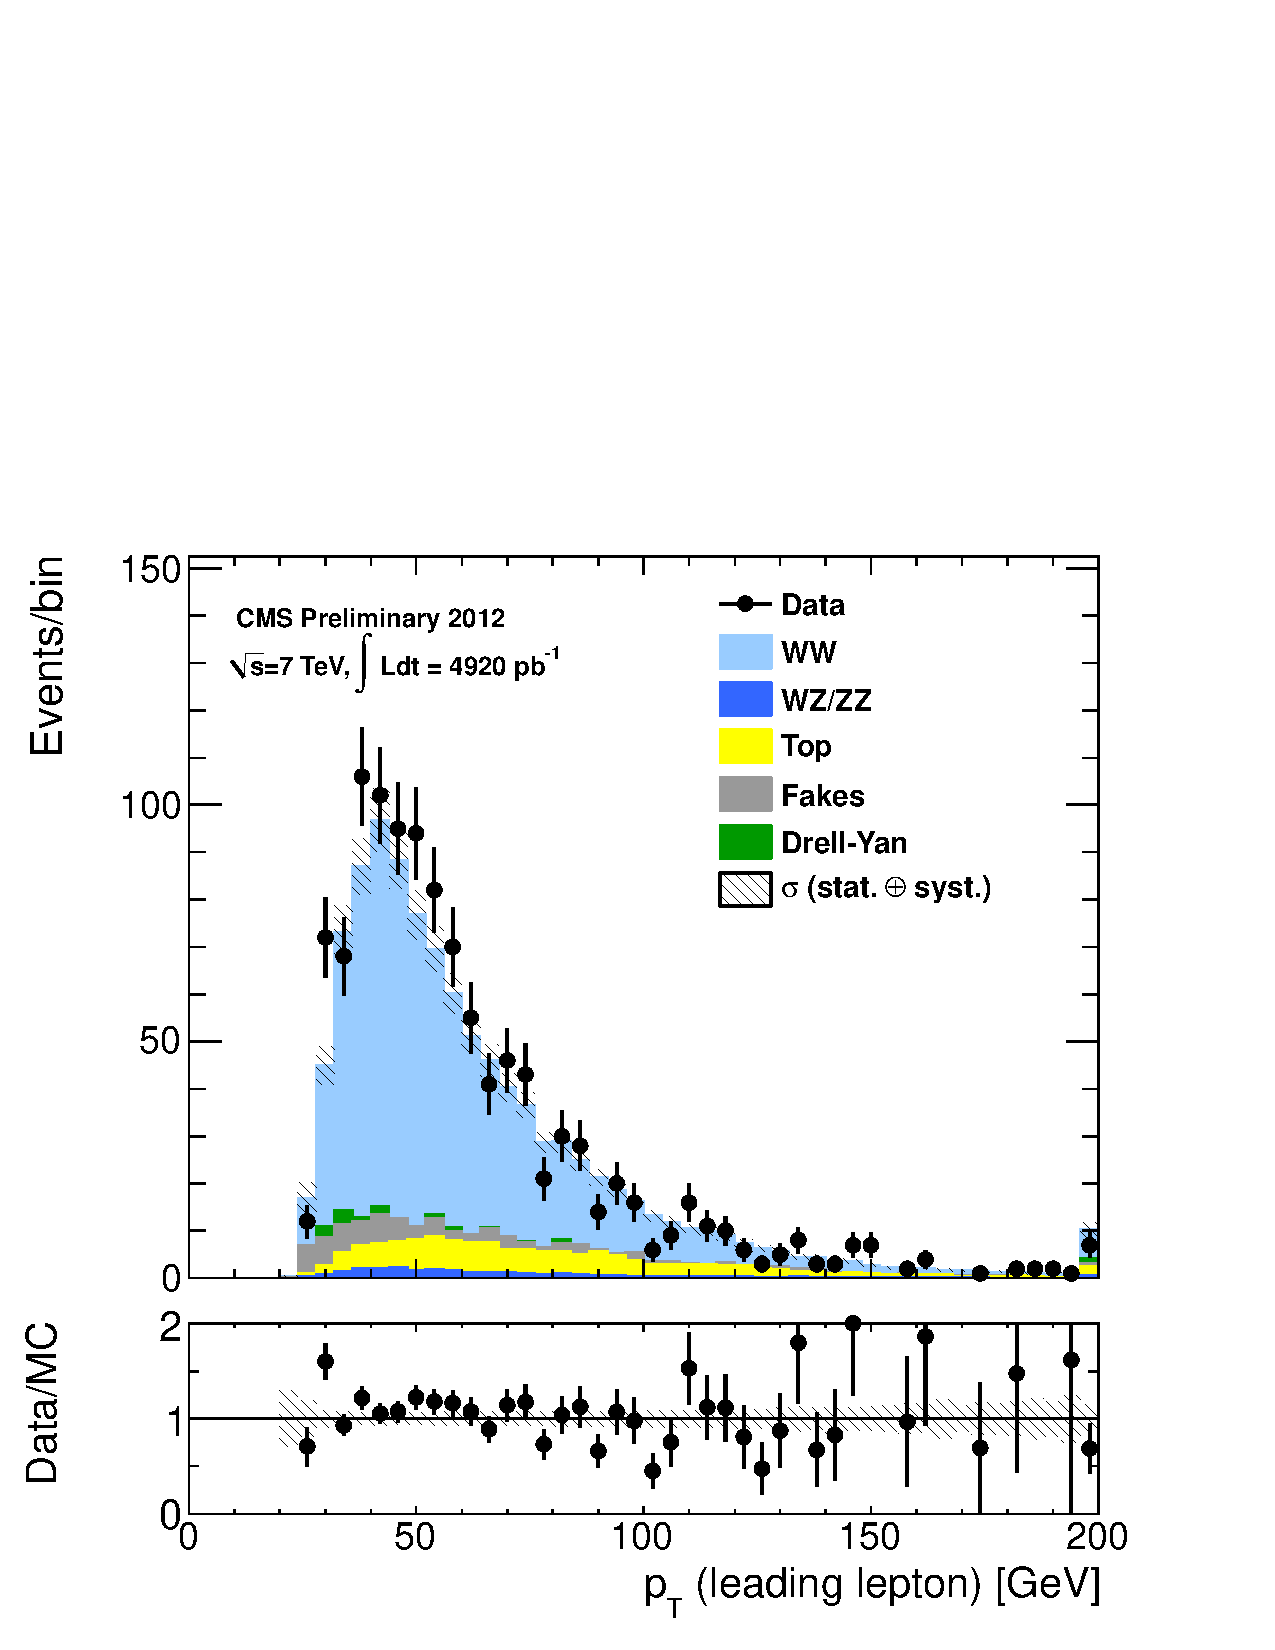
\includegraphics[width=.45\textwidth]{figures/pas_pt1_incl.pdf}}
\subfigure[Log scale]{\label{subfig:pas_pt1_incl_log}
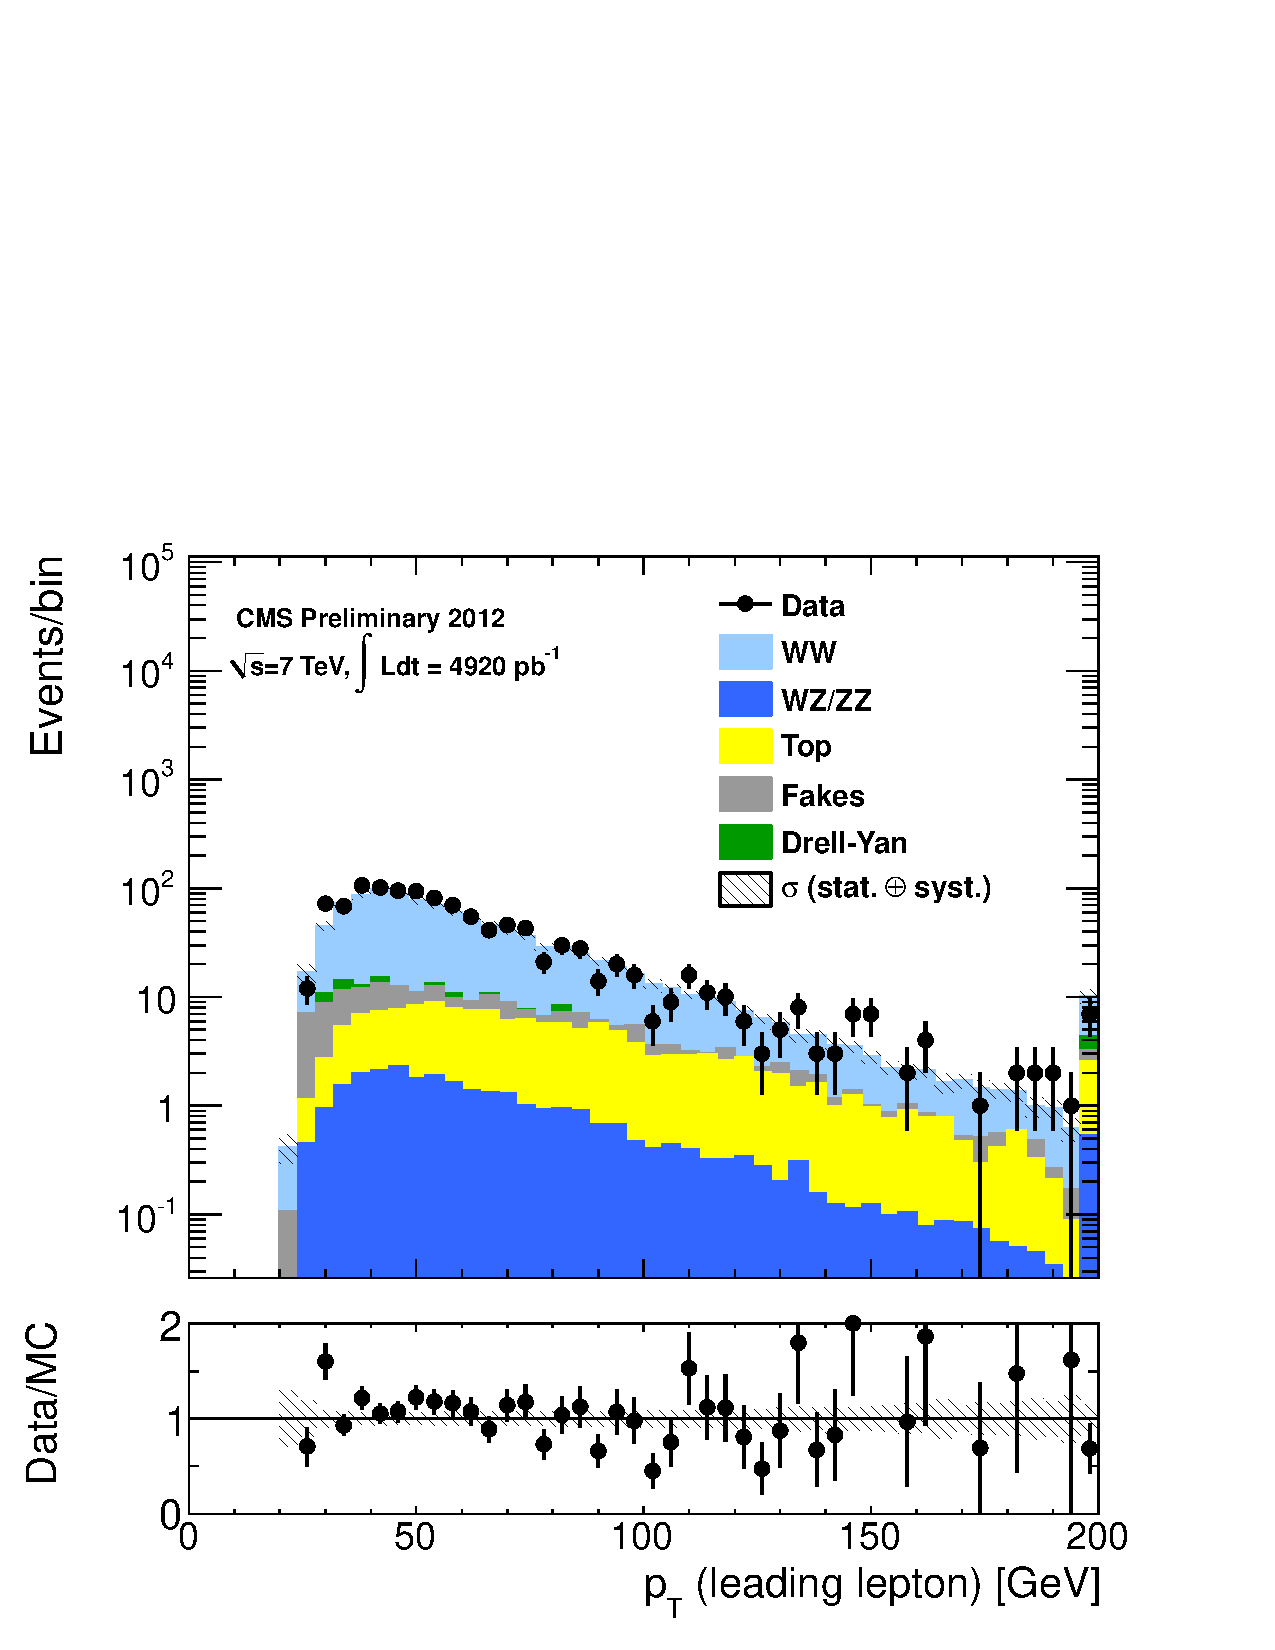
\includegraphics[width=.45\textwidth]{figures/pas_pt1_incl_log.pdf}}
\caption{Leading lepton \pt.}
\label{fig:pas_pt1_incl}
\end{figure}


  
\section{Data Samples}
\label{sec:datasel} 
The data and standard model MC samples used in this analysis are the same 
as in the SM Higgs search~\cite{HWWHCP2012}.
The additional signal samples for $gg\to X\to WW$,
were generated by using
JHUGen~\cite{JHUGen}, with the matrix elements
calculated at LO. The generated LHE files were
interfaced to PYTHIA for showering, hadronization, and the underlying event.
To validate the JHUGen $gg\to X\to WW$ event samples, we also produced 
standard model Higgs boson event samples by using JHUGen.  
These samples are described in Table~\ref{tab:DatasetsMC}. 
The method and results of the validation of JHUGen
are described in Section~\ref{sec:JHUGenval}.

%%%%%%%%%%%%%%%%%%%%%%%%%%%%%%%%%%%%%%%%%%%%%
\begin{table}[!ht]
\begin{center}
{\footnotesize
\begin{tabular}{|c|c|}
\hline
\multicolumn{2}{|c|}{With Pileup: Processed dataset name is always} \\
\multicolumn{2}{|c|}{/Summer12\_DR53X-PU\_S10\_START53\_V7A-v*/AODSIM} \\ 
\hline
 Dataset Description              		&   Primary Dataset Name  \\ 
\hline
$gg\to H\to WW\to (l\nu)(l\nu)$, $l=e,\mu$      & SMHiggsToWWTo2L2Nu\_M-125\_8TeV-jhu-pythia6 \\ 
$gg\to H\to WW\to (l\nu)(\tau\nu)$, $l=e,\mu$   & SMHiggsToWWToLTau2Nu\_M-125\_8TeV-jhu-pythia6 \\
$gg\to H\to WW\to (\tau\nu)(\tau\nu)$           & SMHiggsToWWToTauTau2Nu\_M-125\_8TeV-jhu-pythia6 \\
$gg\to \text{Graviton}\to WW\to (l\nu)(l\nu)$, $l=e,\mu$      & Graviton2PMToWWTo2L2Nu\_M-125\_8TeV-jhu-pythia6 \\ 
$gg\to \text{Graviton}\to WW\to (l\nu)(\tau\nu)$, $l=e,\mu$   & Graviton2PMToWWToLTau2Nu\_M-125\_8TeV-jhu-pythia6 \\
$gg\to \text{Graviton}\to WW\to (\tau\nu)(\tau\nu)$           & Graviton2PMToWWToTauTau2Nu\_M-125\_8TeV-jhu-pythia6 \\
\hline
\end{tabular}
}
\label{tab:DatasetsMC}
\caption{Summary of additional Monte Carlo datasets used at $\sqrt{s} = 8~\TeV$. 
Other samples are described in detail in~\cite{HWWHCP2012}. The same set of 
corresponding samples at $\sqrt{s} = 7~\TeV$ are also available and used in this study.}
\end{center}
\end{table}
%%%%%%%%%%%%%%%%%%%%%%%%%%%%%%%%%%%%%%%%%%%%%

\subsection{JHUGen validation}
\label{sec:JHUGenval}

To validate JHUGen, we compared the main kinematic distributions between JHUGen and
MCFM at the generator level, and to the Powheg-Pythia samples used in the
SM Higgs search at the reconstruction level.

Figure~\ref{fig:jhuvsmcfm} compares the main kinematic observables at generator 
level between the JHUGen and MCFM for events without any cuts. 
Both samples are generated with the Higgs boson produced at rest. 
We observe good agreement within a few percent in the bulk of the two distributions. 

%%%%%%%%%%%%%%%%%%%%%%%%%%%%%%%%%%%%%%%%%%%%%
\begin{figure}[!hbtp]
\centering
\subfigure[Leading Lepton $\pt$]{
\centering
\label{subfig:leadleppt}
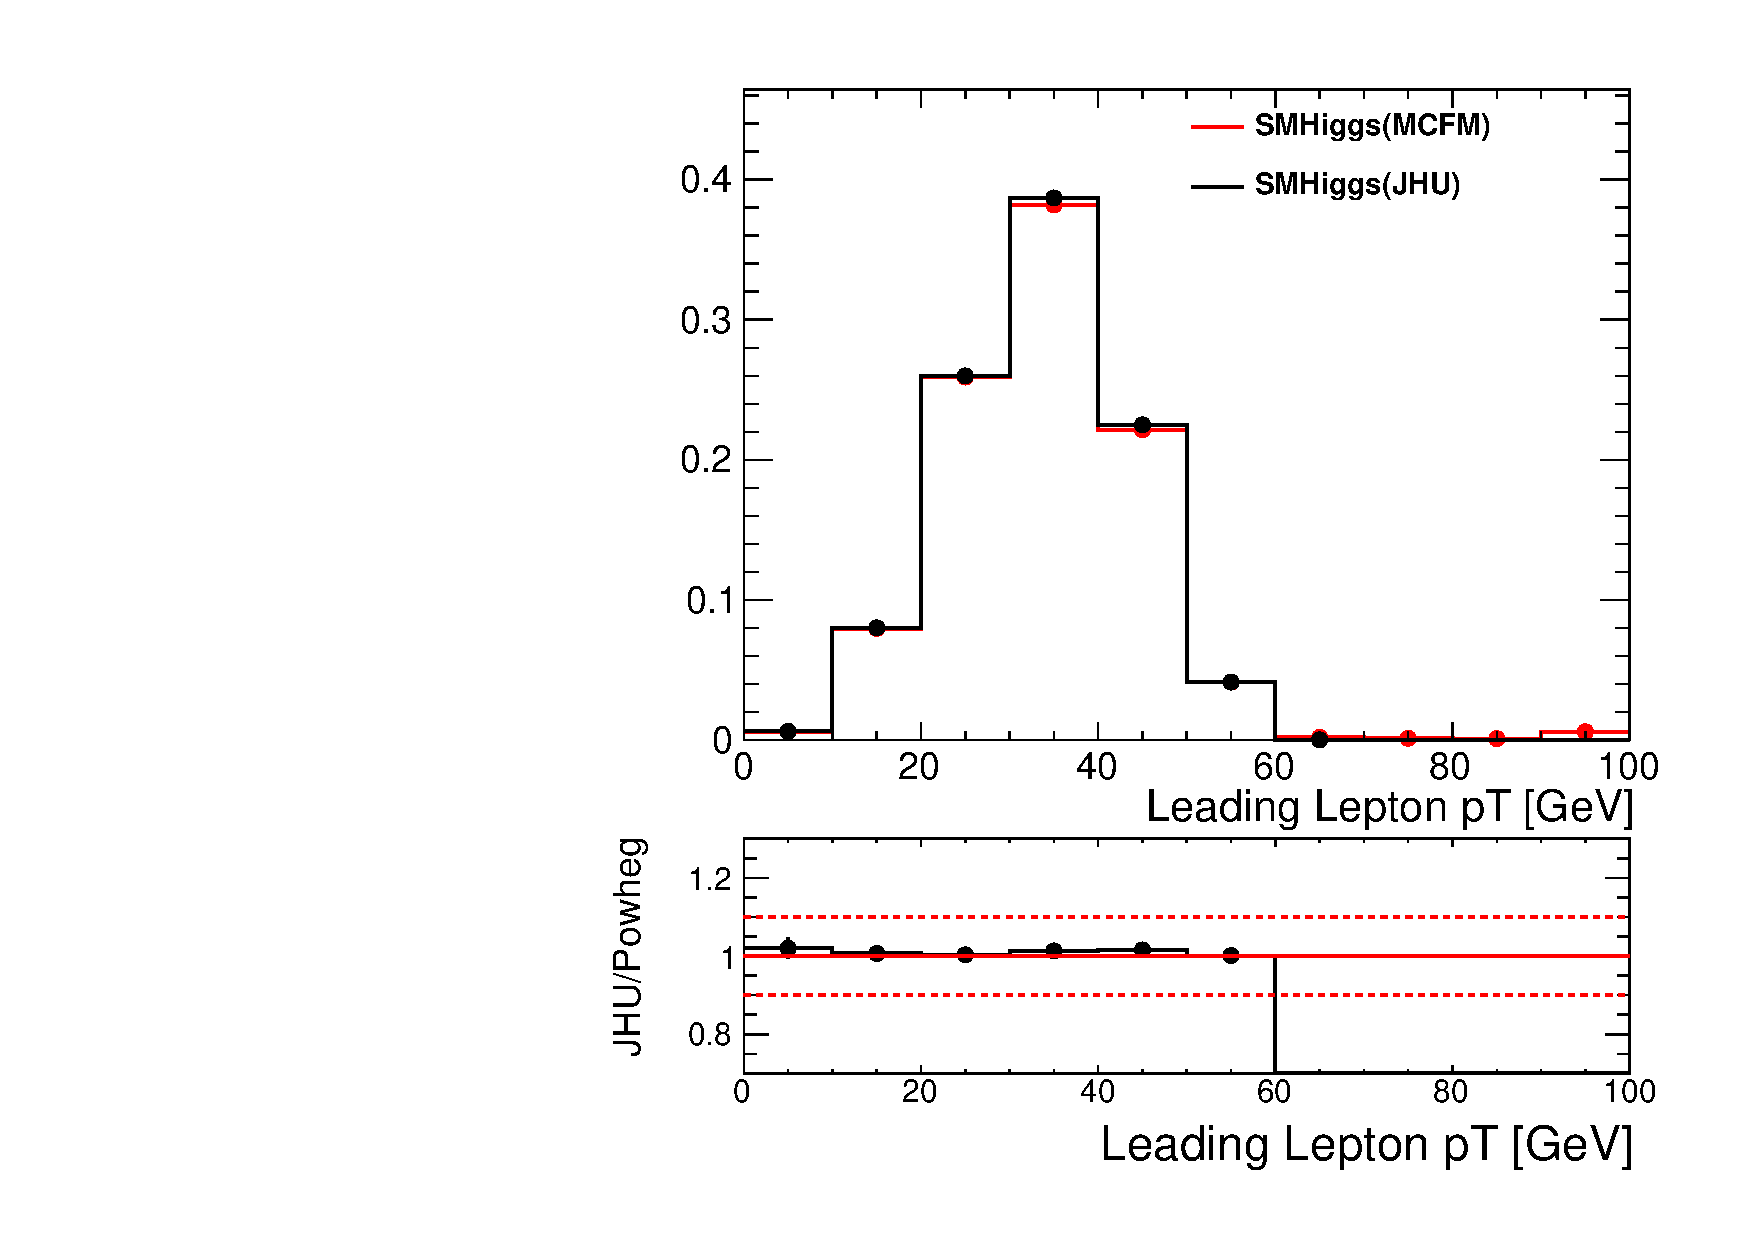
\includegraphics[width=.3\textwidth]{figures/leadleppt_jhuvsmcfm.pdf}
}
\subfigure[Trailing Lepton $\pt$]{
\centering
\label{subfig:trailleppt}
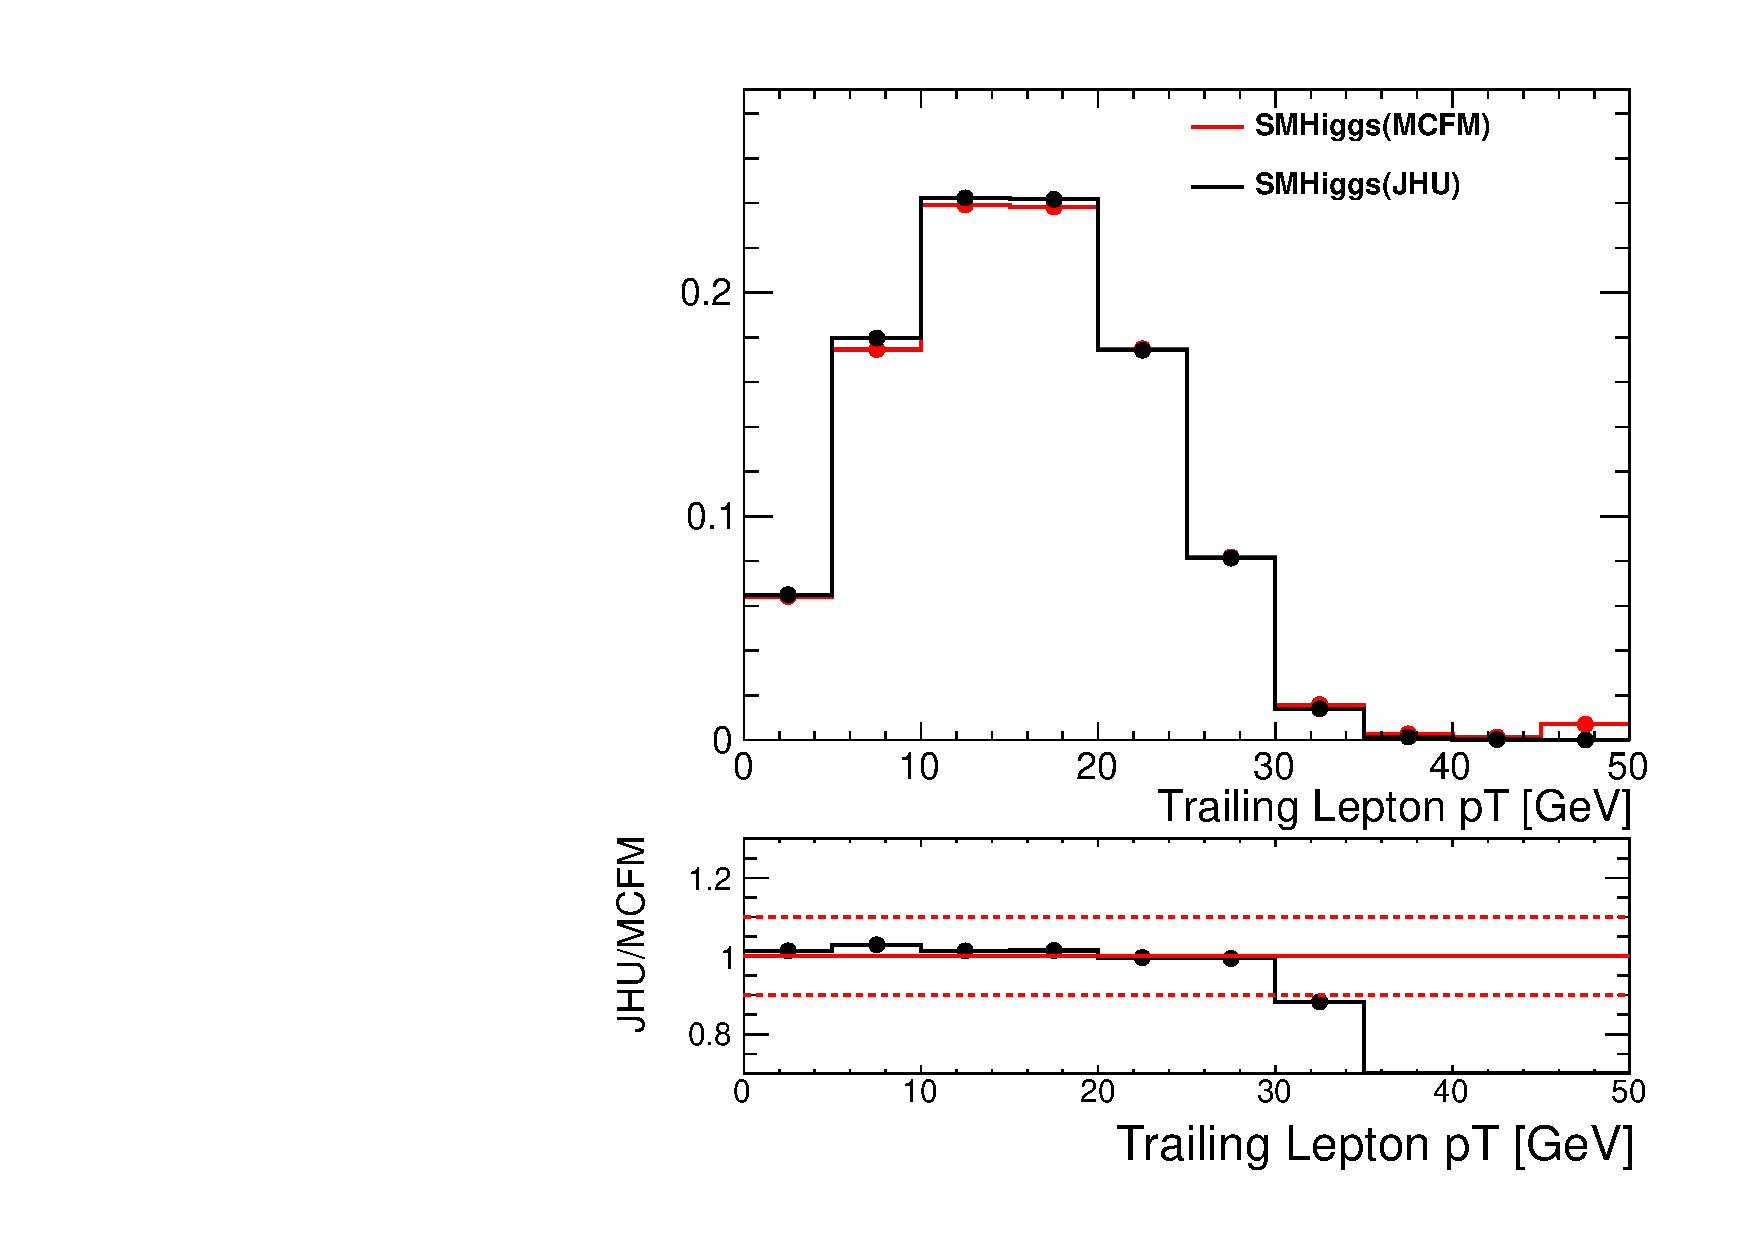
\includegraphics[width=.3\textwidth]{figures/trailleppt_jhuvsmcfm.pdf}
}
\subfigure[Leading Lepton $\eta$]{
\centering
\label{subfig:leadlepeta}
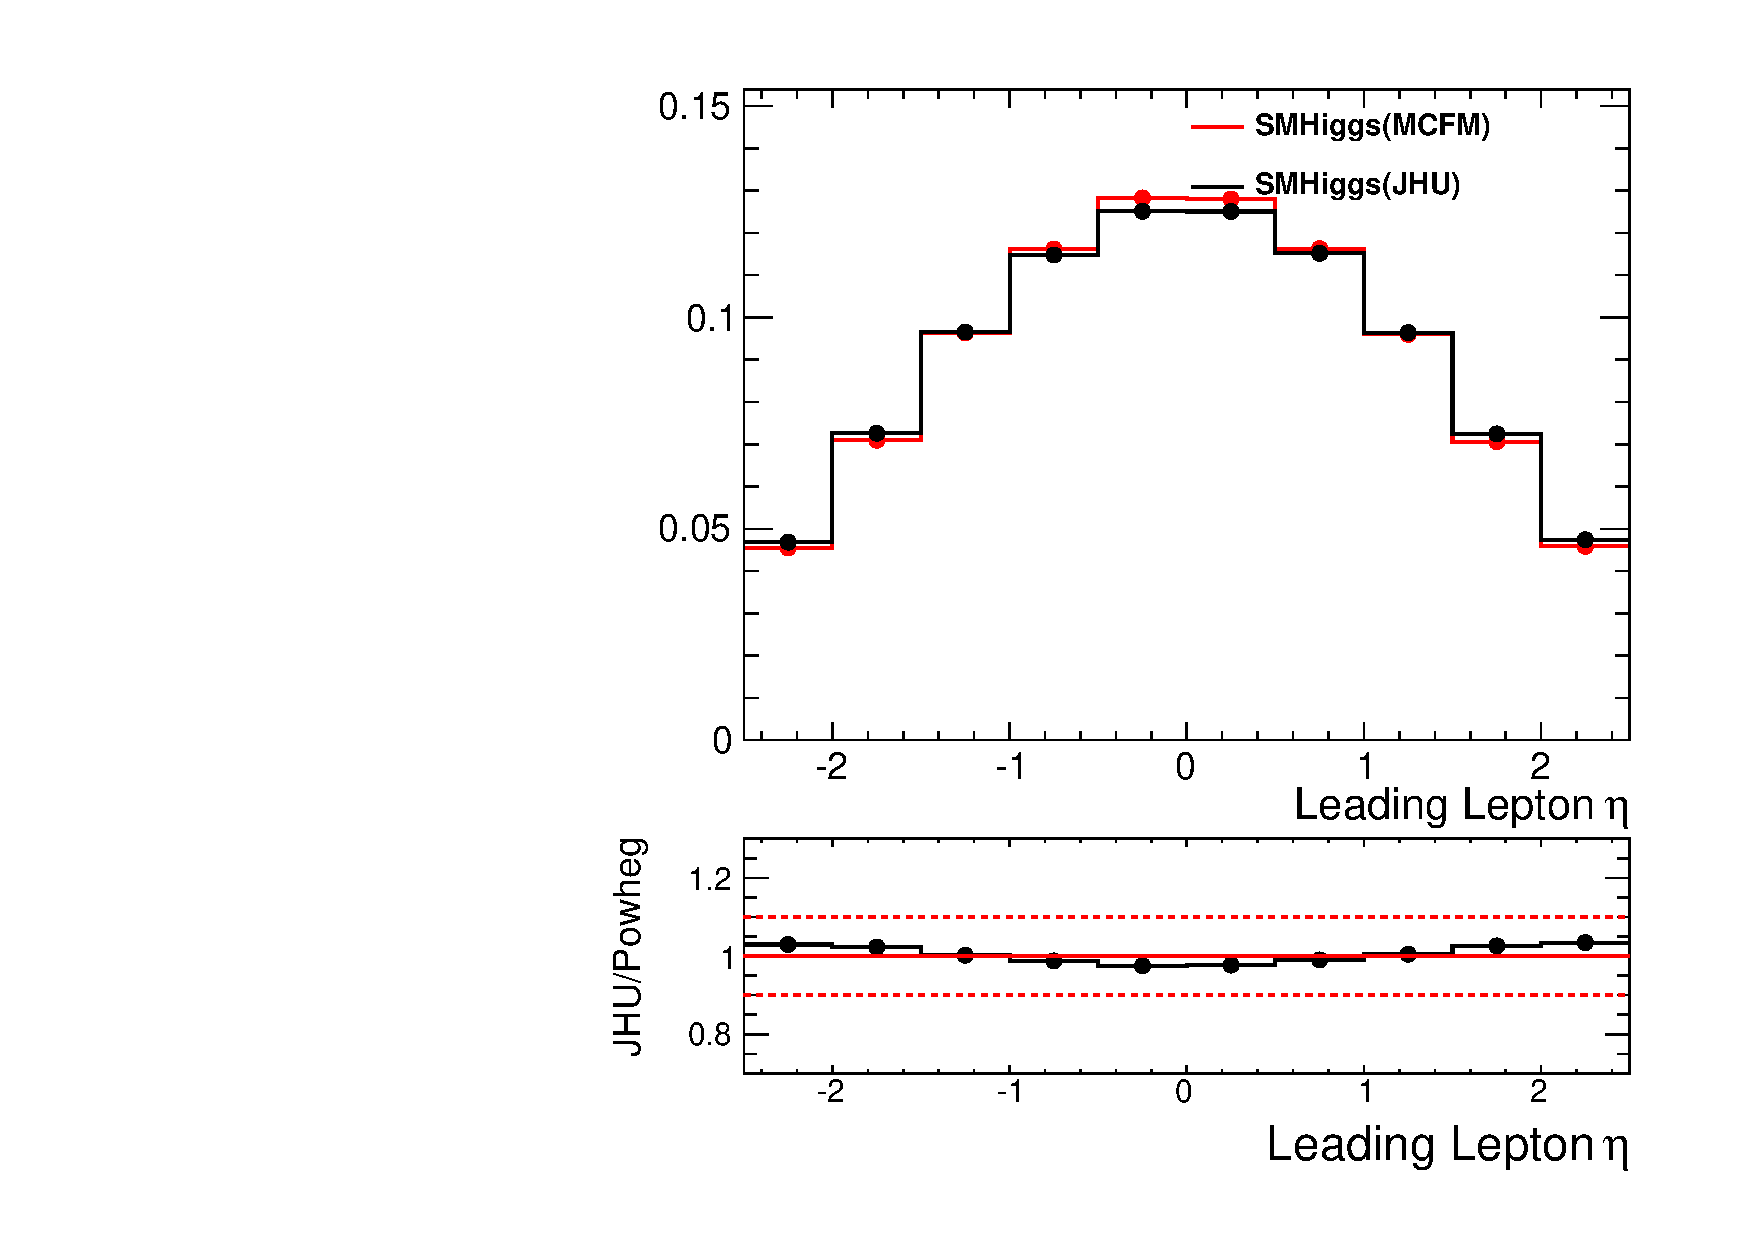
\includegraphics[width=.3\textwidth]{figures/leadlepeta_jhuvsmcfm.pdf}
} \\
\subfigure[Trailing Lepton $\eta$]{
\centering
\label{subfig:traillepeta}
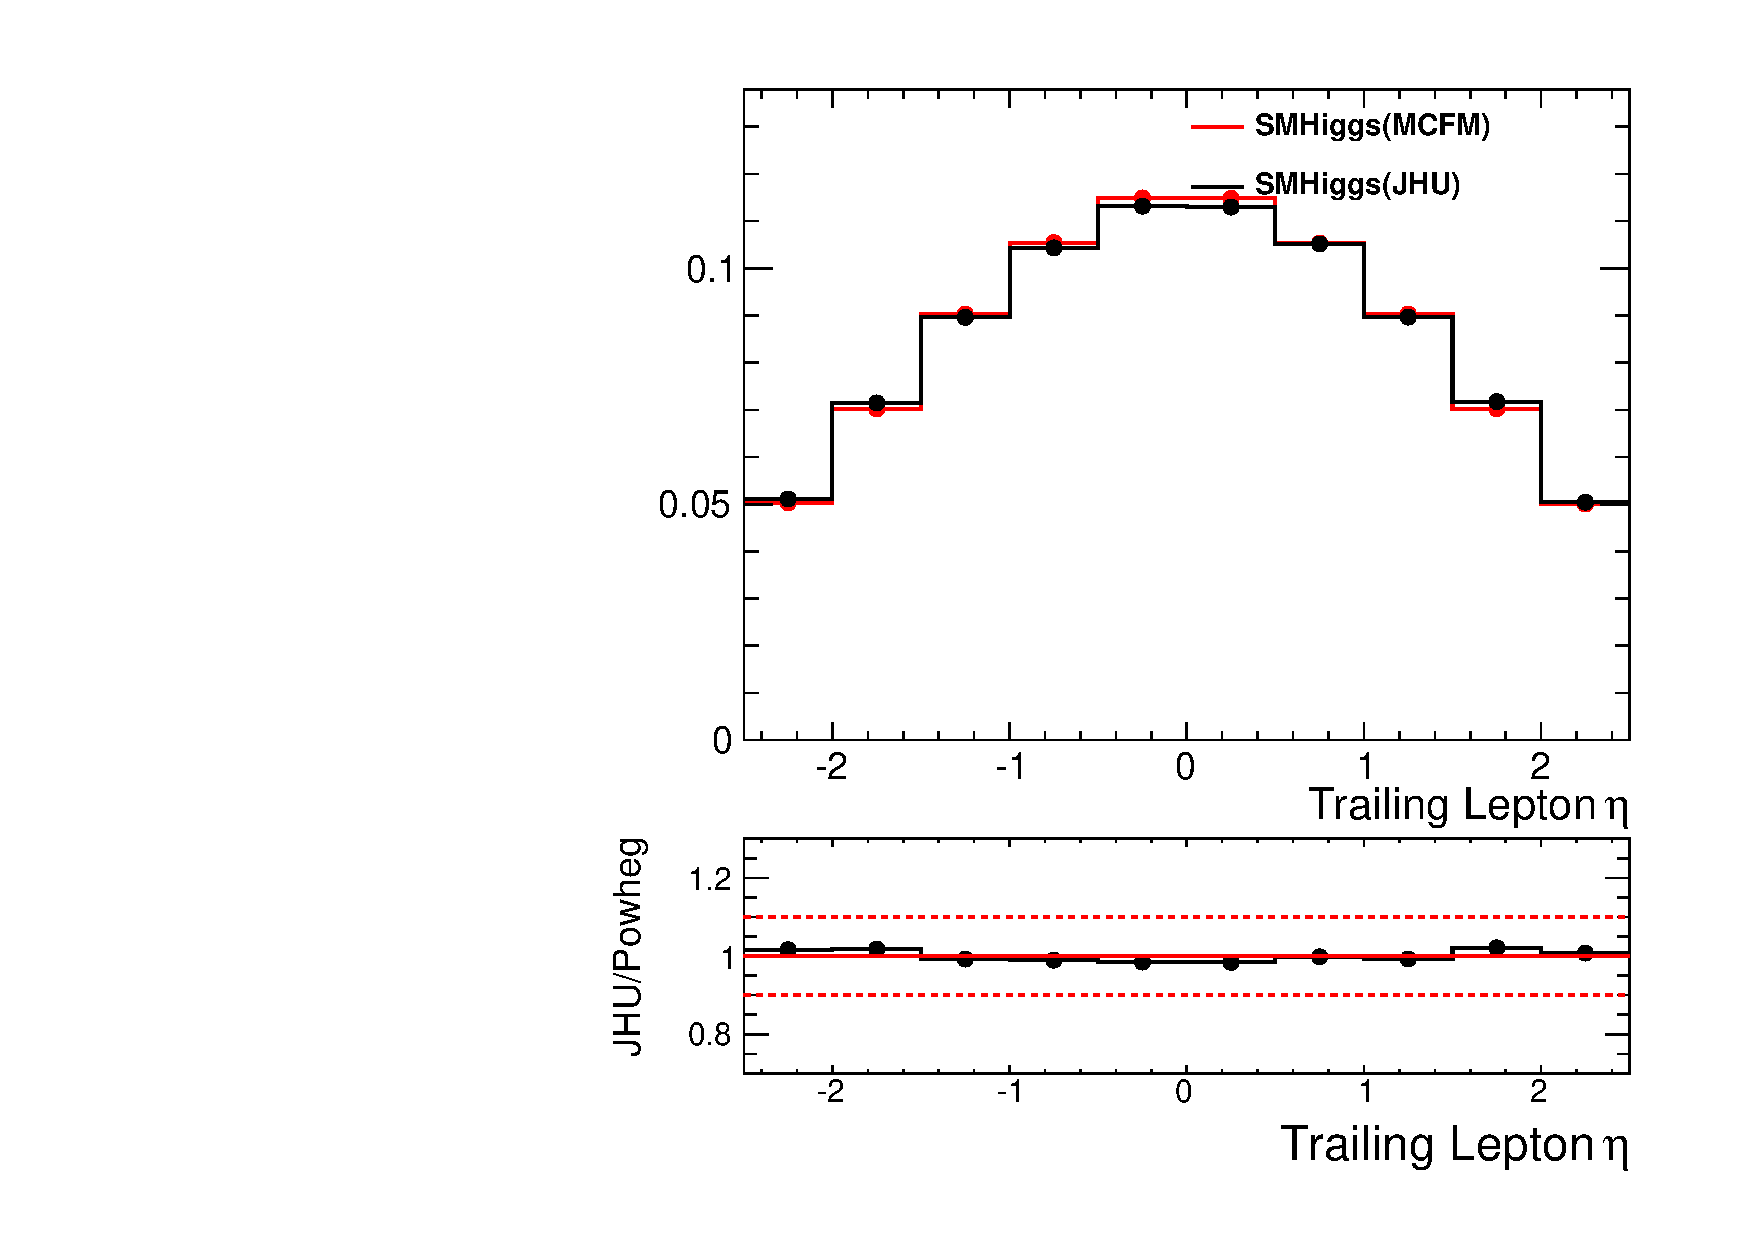
\includegraphics[width=.3\textwidth]{figures/traillepeta_jhuvsmcfm.pdf}
}
\subfigure[Dilepton mass]{
\centering
\label{subfig:mll}
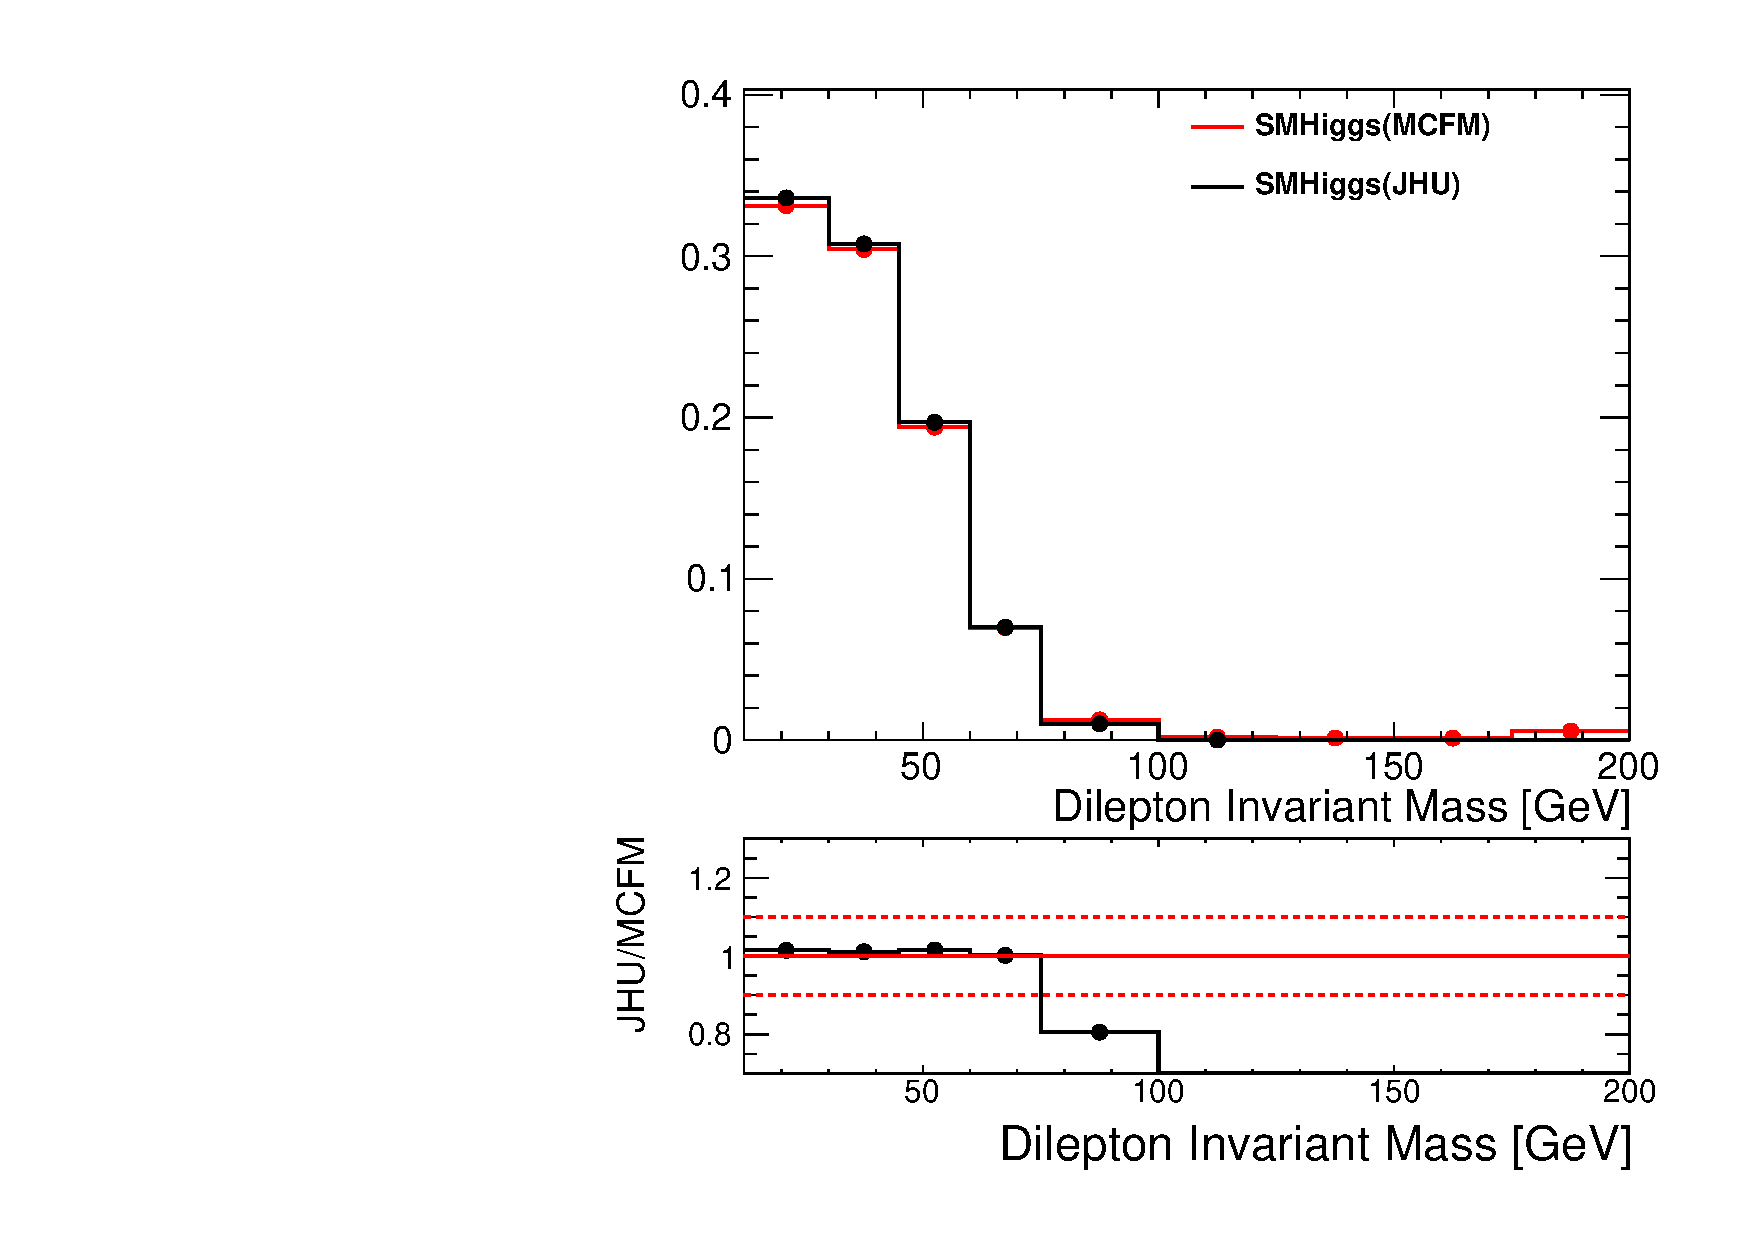
\includegraphics[width=.3\textwidth]{figures/mll_jhuvsmcfm.pdf}
} 
\subfigure[Transverse Higgs Mass]{
\centering
\label{subfig:mt}
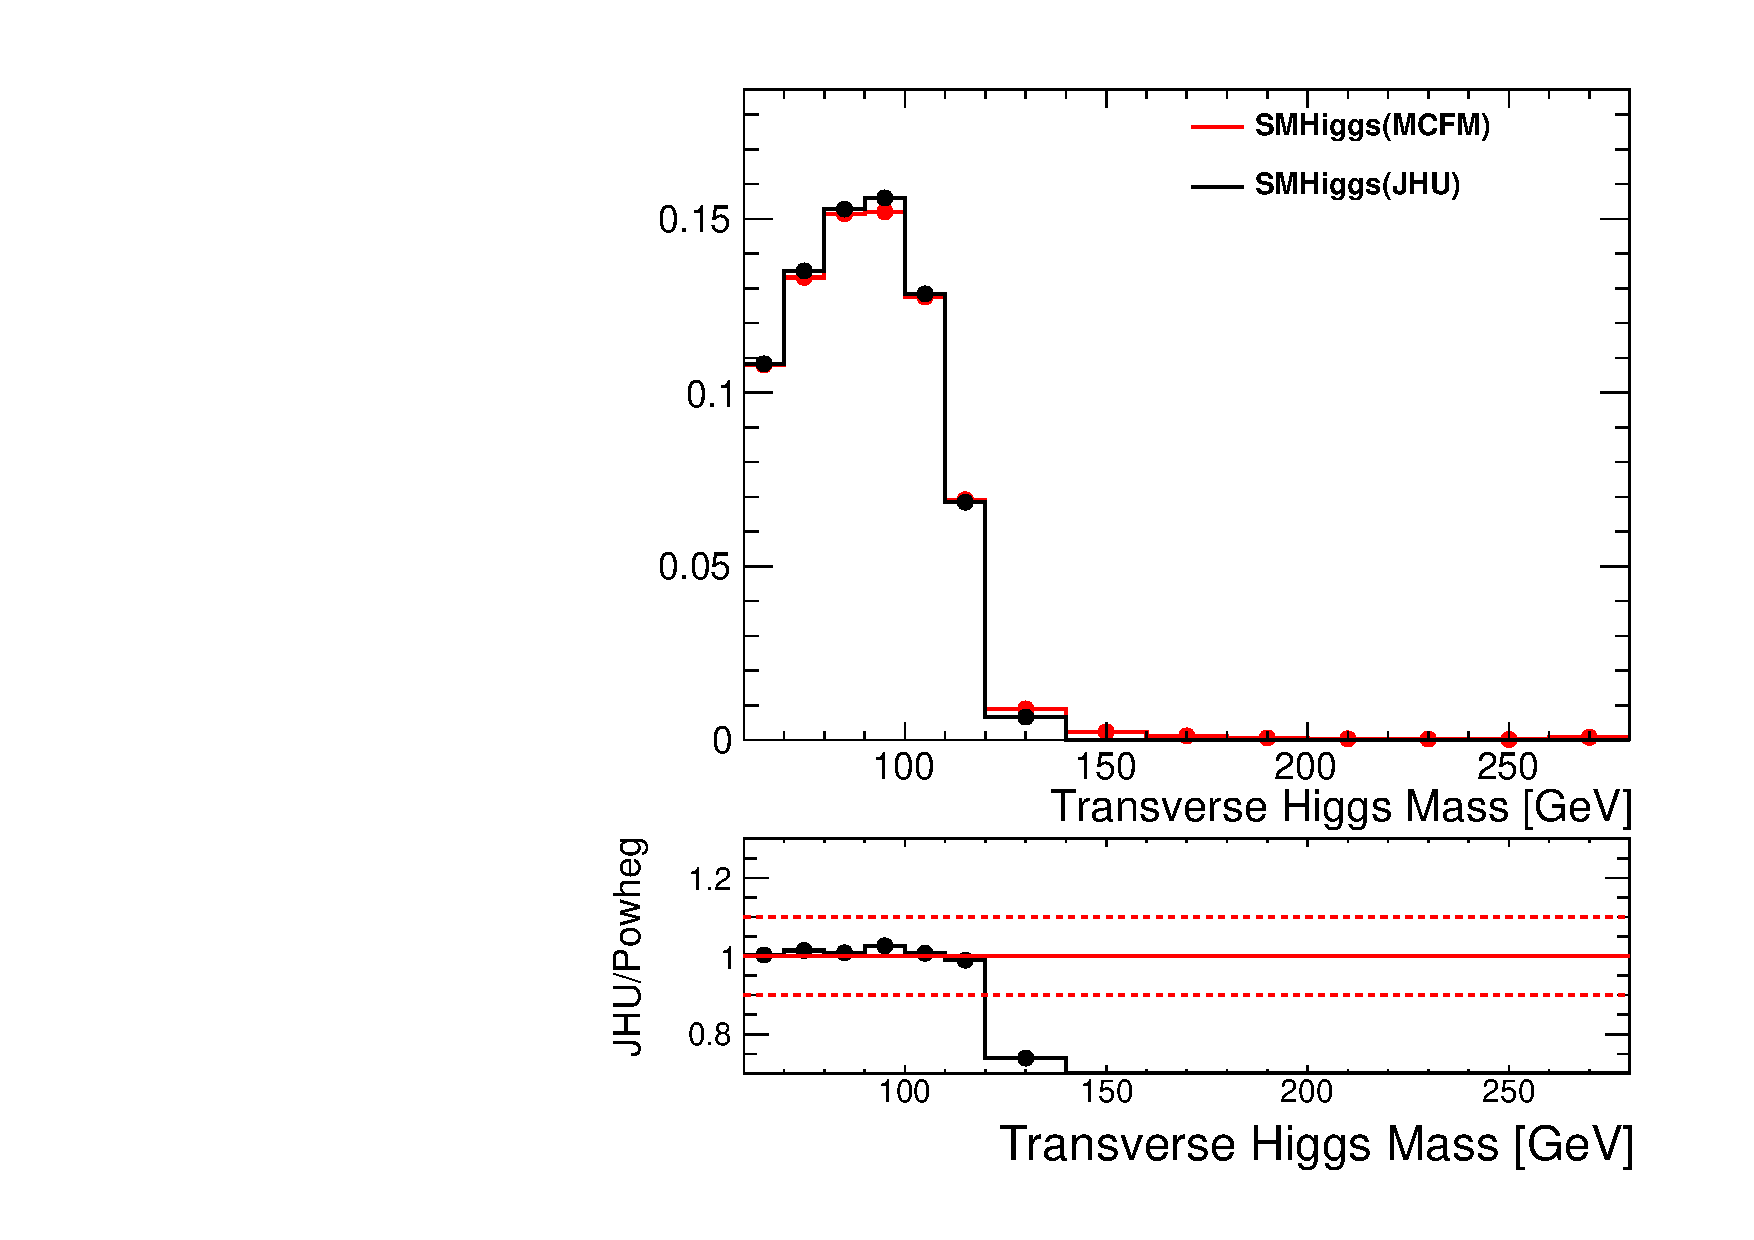
\includegraphics[width=.3\textwidth]{figures/mt_jhuvsmcfm.pdf}
}\\
\subfigure[Dilepton $\pt$]{
\centering
\label{subfig:dilpt}
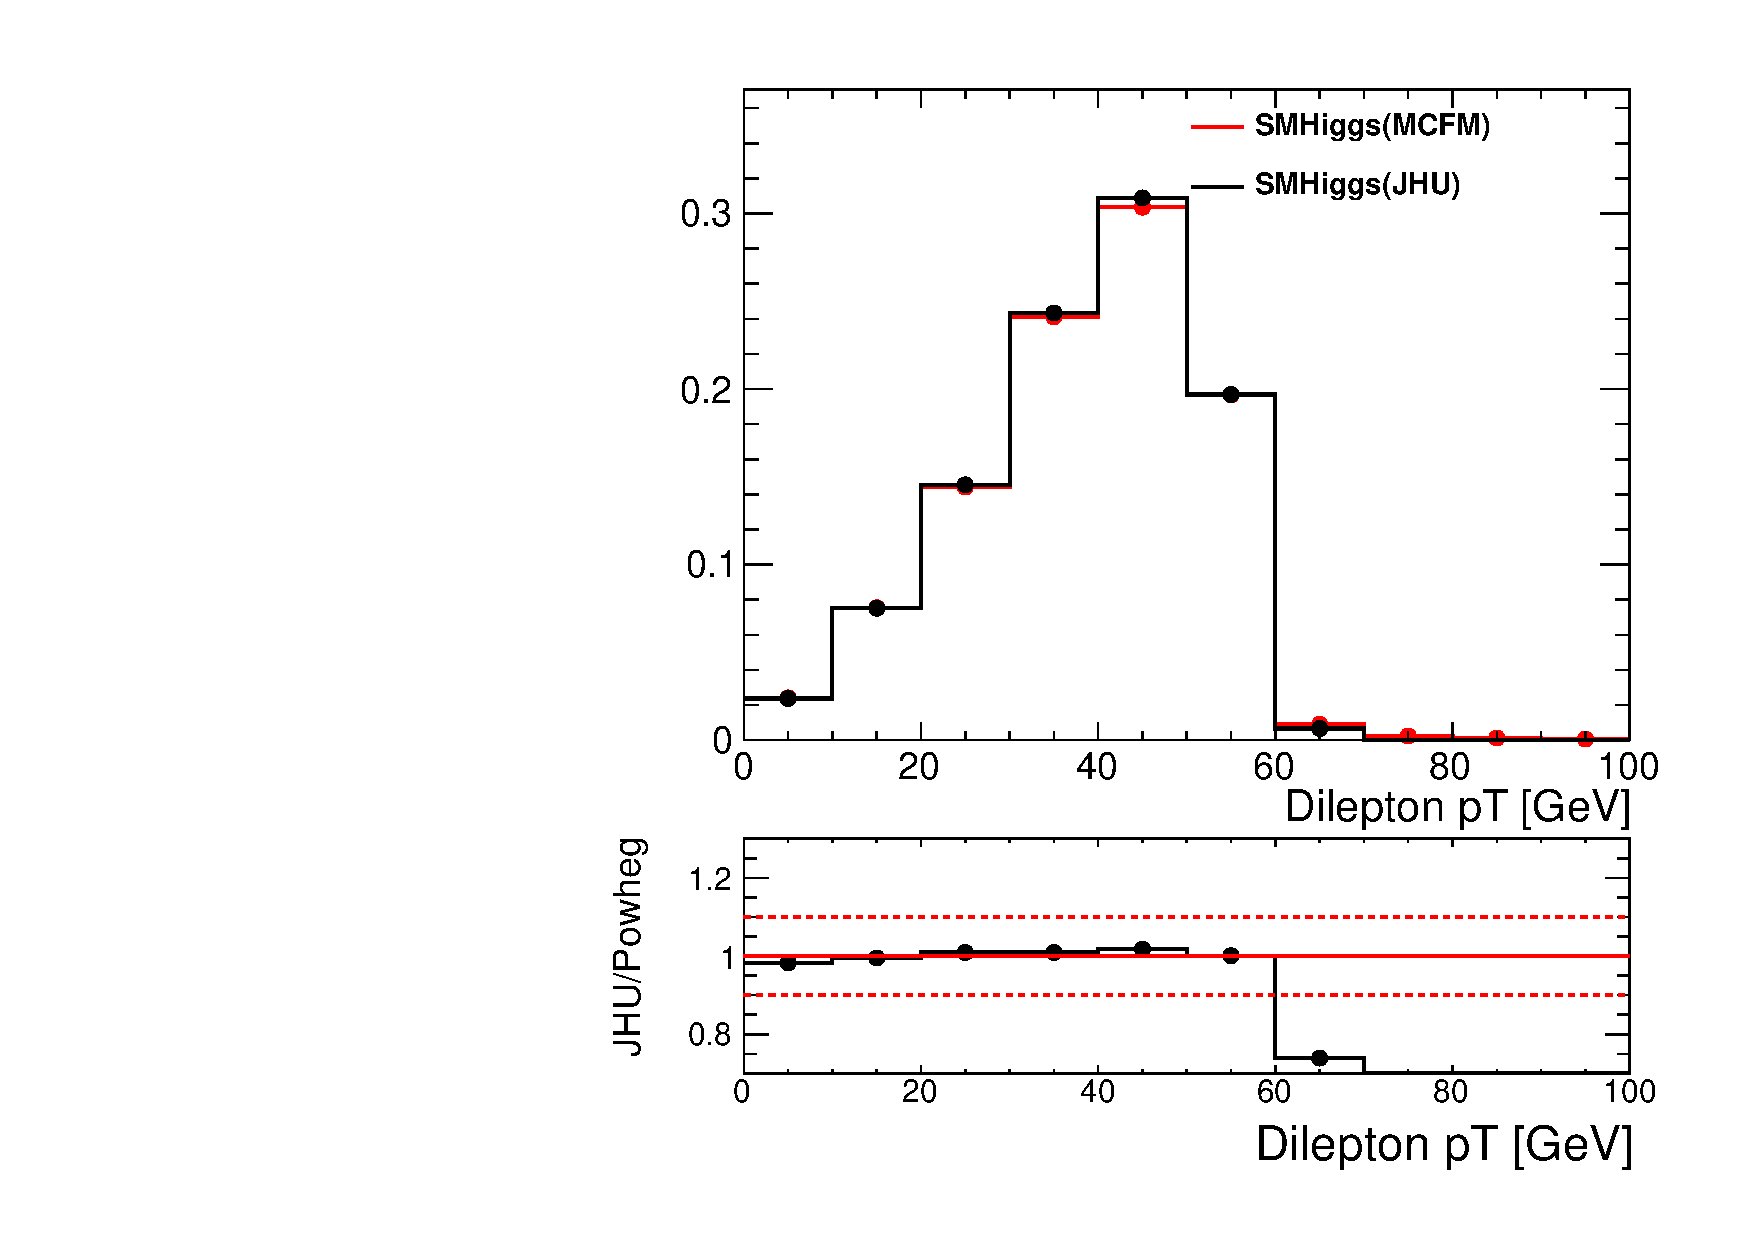
\includegraphics[width=.3\textwidth]{figures/dilpt_jhuvsmcfm.pdf}
}
\subfigure[Neutrino $\pt$]{
\centering
\label{subfig:met}
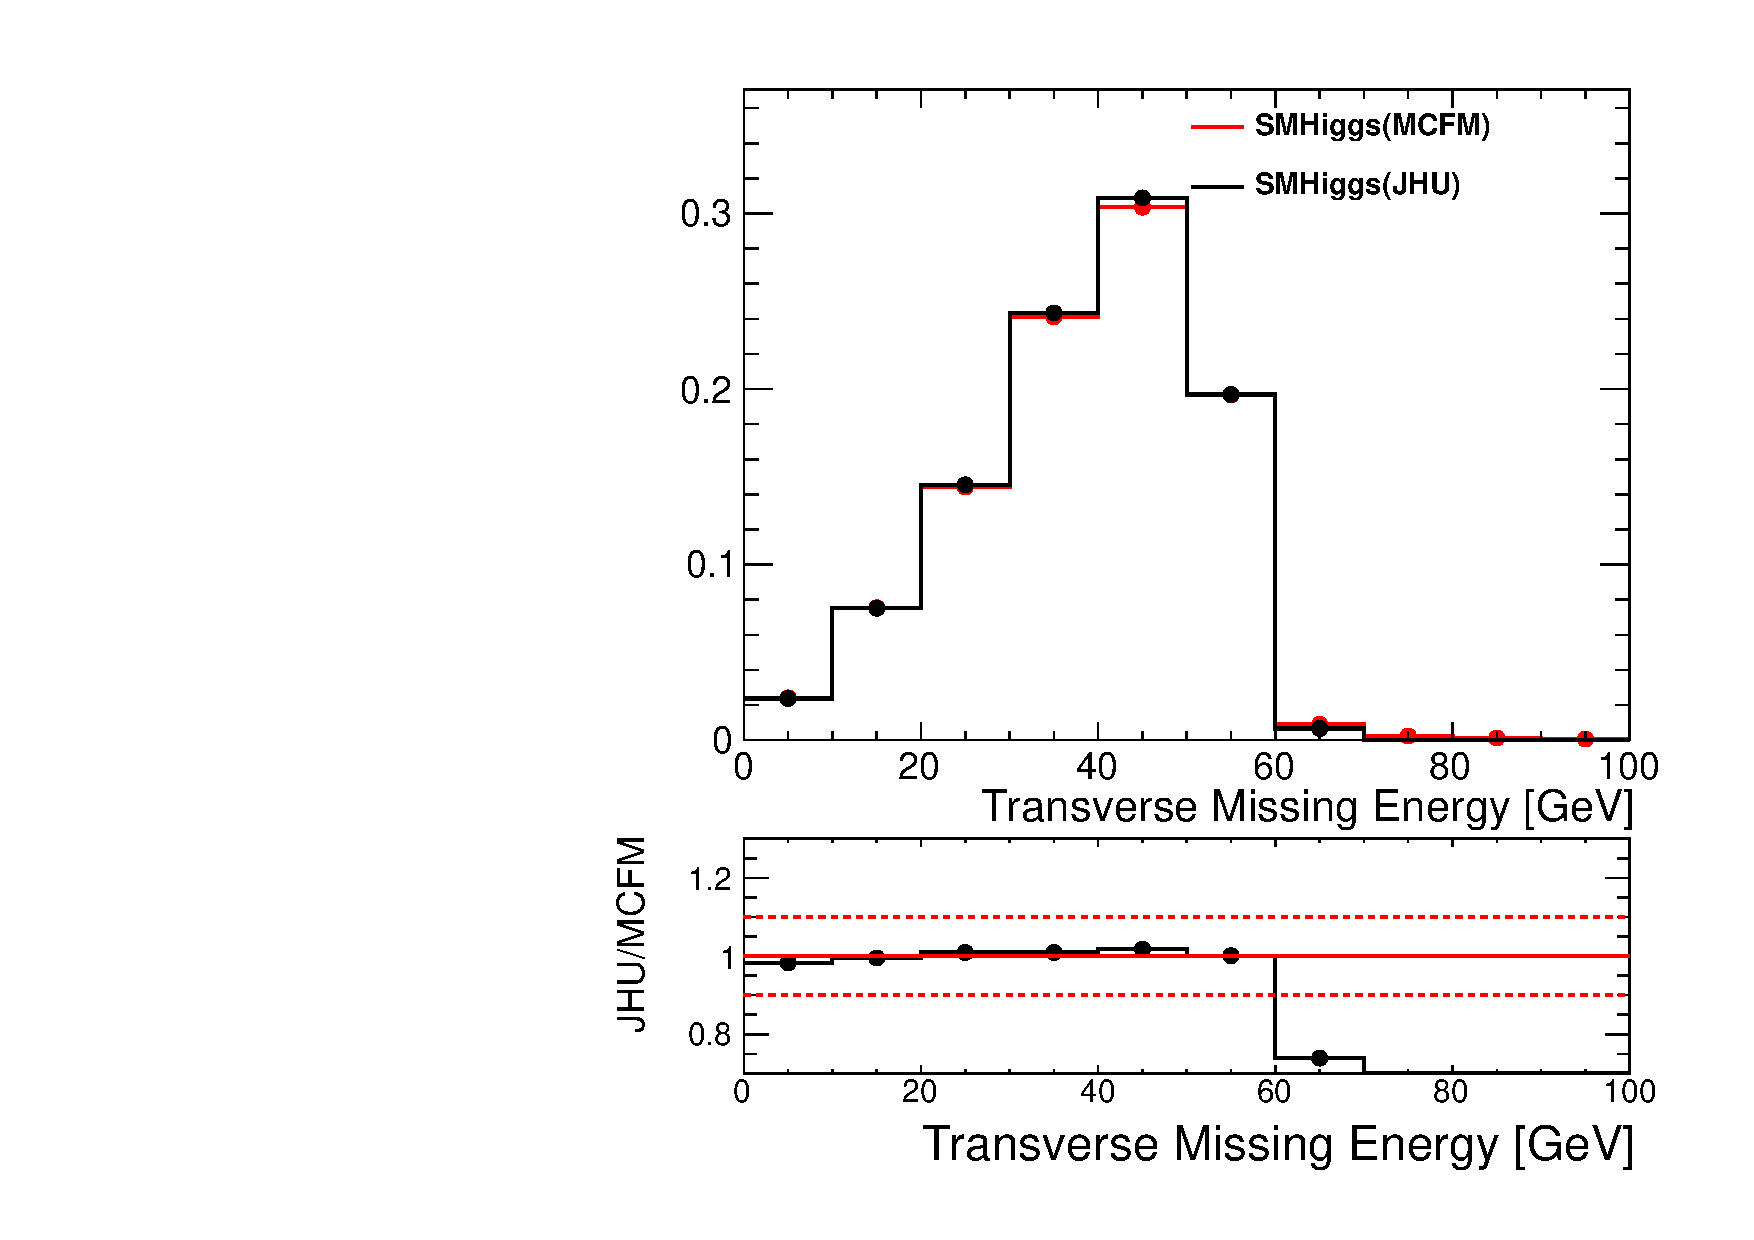
\includegraphics[width=.3\textwidth]{figures/met_jhuvsmcfm.pdf}
}
\subfigure[$\Delta\phi_{\ell\ell}$]{
\centering
\label{subfig:met}
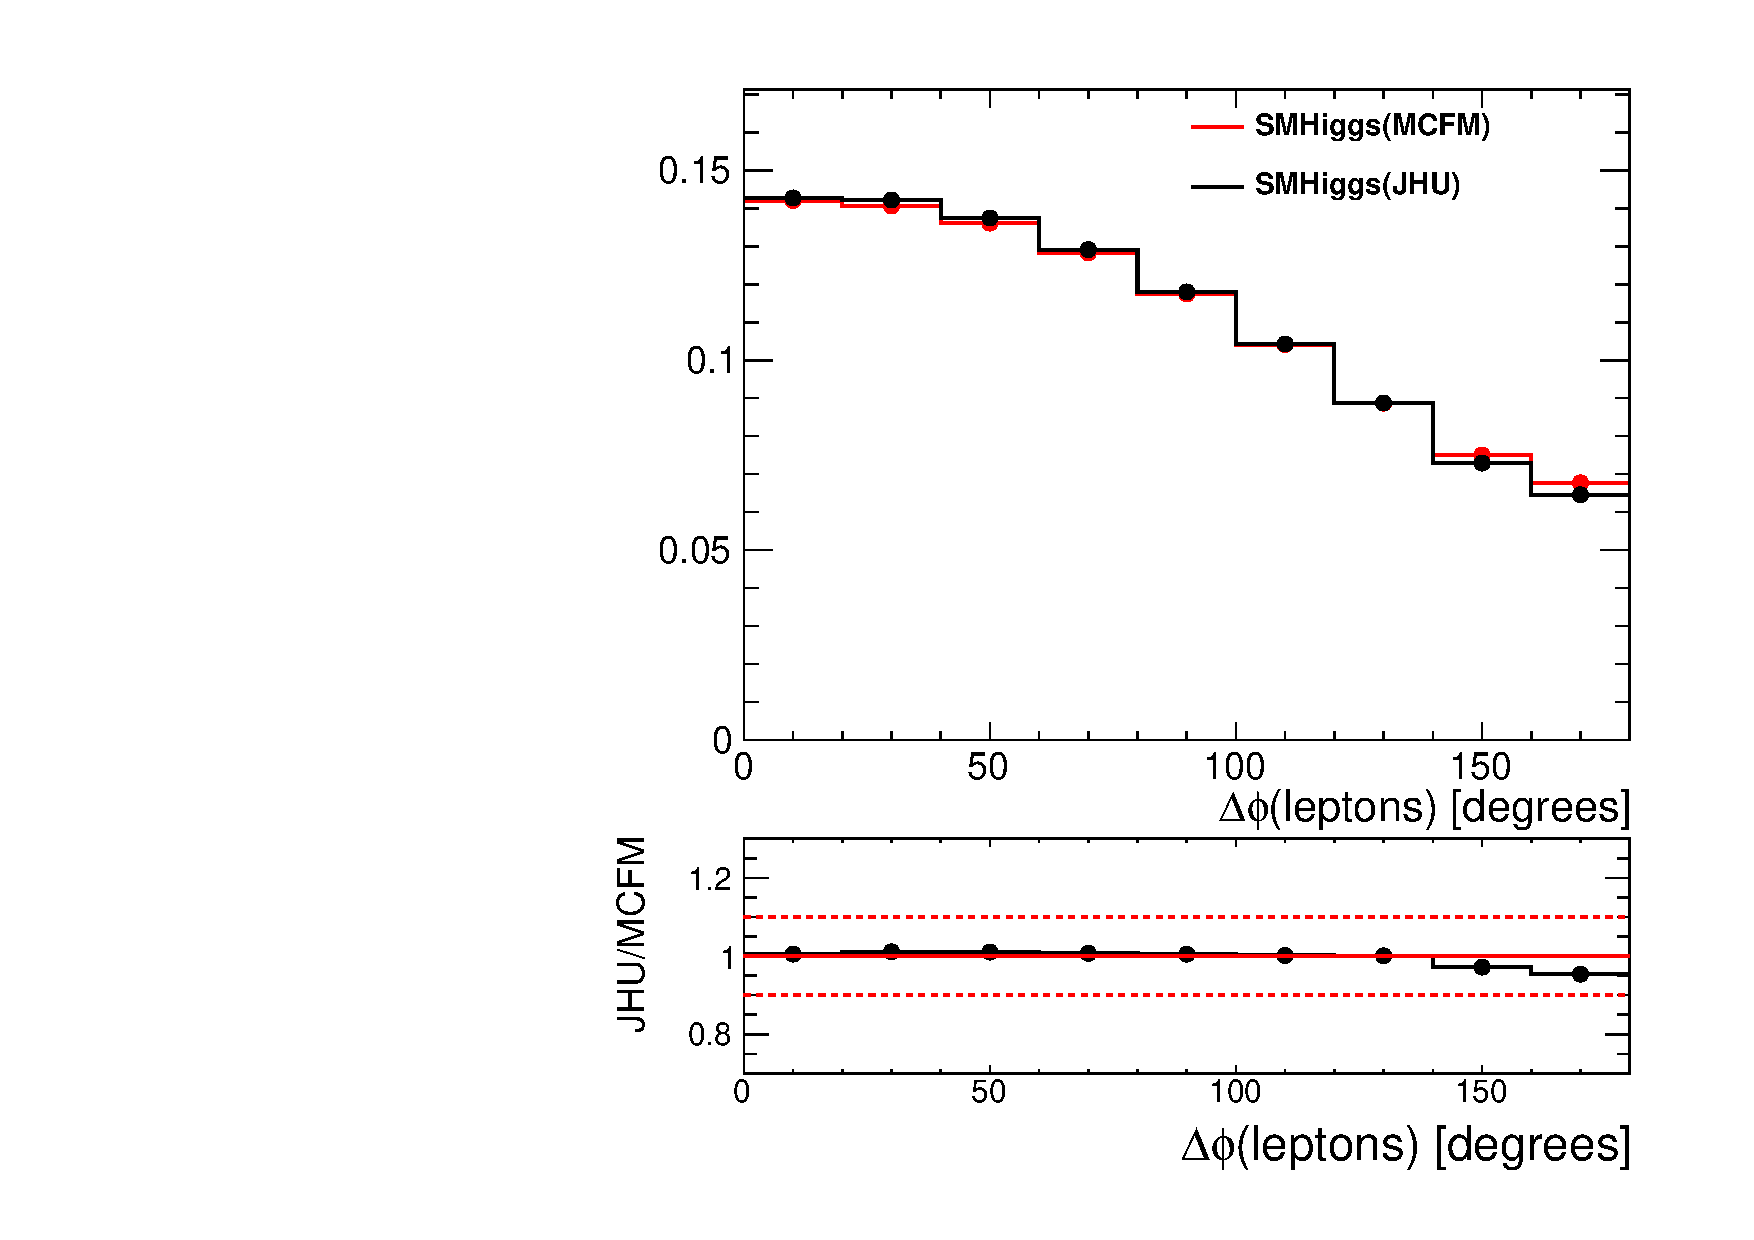
\includegraphics[width=.3\textwidth]{figures/dphill_jhuvsmcfm.pdf}
}\\
\caption{Gerator level kinematic distributions (normalized to 1) of SM Higgs 
comparing JHUGen and MCFM without any cuts. Both samples are generated with 
the Higgs boson produced at rest. }
\label{fig:jhuvsmcfm}
\end{figure}
%%%%%%%%%%%%%%%%%%%%%%%%%%%%%%%%%%%%%%%%%%%%%

Figure~\ref{fig:higgspt_0j} shows the Higgs boson $\pt$ and the leading jet 
$\pt$ distributions for the SM Higgs hypothesis comparing the 
JHUGen-Pythia and Powheg-Pythia~\cite{powheg} samples, after applying the full 
simulation, reconstruction and event selection. The two generators agree within 10\%. 
This level of agreement is expected because Powheg uses
NLO matrix element calculations. The effect on the main kinematic observables due to 
the difference in Higgs $\pt$ however is smaller, as shown in Figure~\ref{fig:higgskin_0j}. 

%To account for the missing higher order effects in JHUGen,
%we reweight the two-dimensional templates ($m_T-m_{\ell\ell}$) 
%in the final analysis from JHUGen-Pythia to match to the predictions of Powheg-Pythia for the SM Higgs hypothesis. 
%The relative difference between JHUGen and Powheg in the SM Higgs boson hypothesis is then applied to the other signal hypotheses as well, because we 
%assume the effects are similar as all resonances are colorless objects. 
%%Therefore the missing higher 
%order effects are similar between different hypotheses. 
Figure~\ref{fig:gravvshiggspt_0j} shows the resonance $\pt$ and 
the leading jet $\pt$ distributions comparing the spin-2 
graviton and the SM Higgs hypothesis generated with the JHUGen-Pythia. 
The two hypotheses agree within a few percent in the bulk of the distributions,
smaller than the differences between Powheg-Pythia and JHUGen-Pythia 
in the SM Higgs hypothesis. 
For the moment we use the same theoretical uncertainties as in the SM Higgs 
analysis for the $2_{\text min}^+$ analysis..
%An additional systematic uncertainty due to this difference is assigned,
%as described in Section~\ref{sec:systematics}. 

%%%%%%%%%%%%%%%%%%%%%%%%%%%%%%%%%%%%%%%%%%%%%
\begin{figure}[!hbtp]
\centering
\subfigure[Higgs $\pt$]{
\centering
\label{subfig:higgspt_0j}
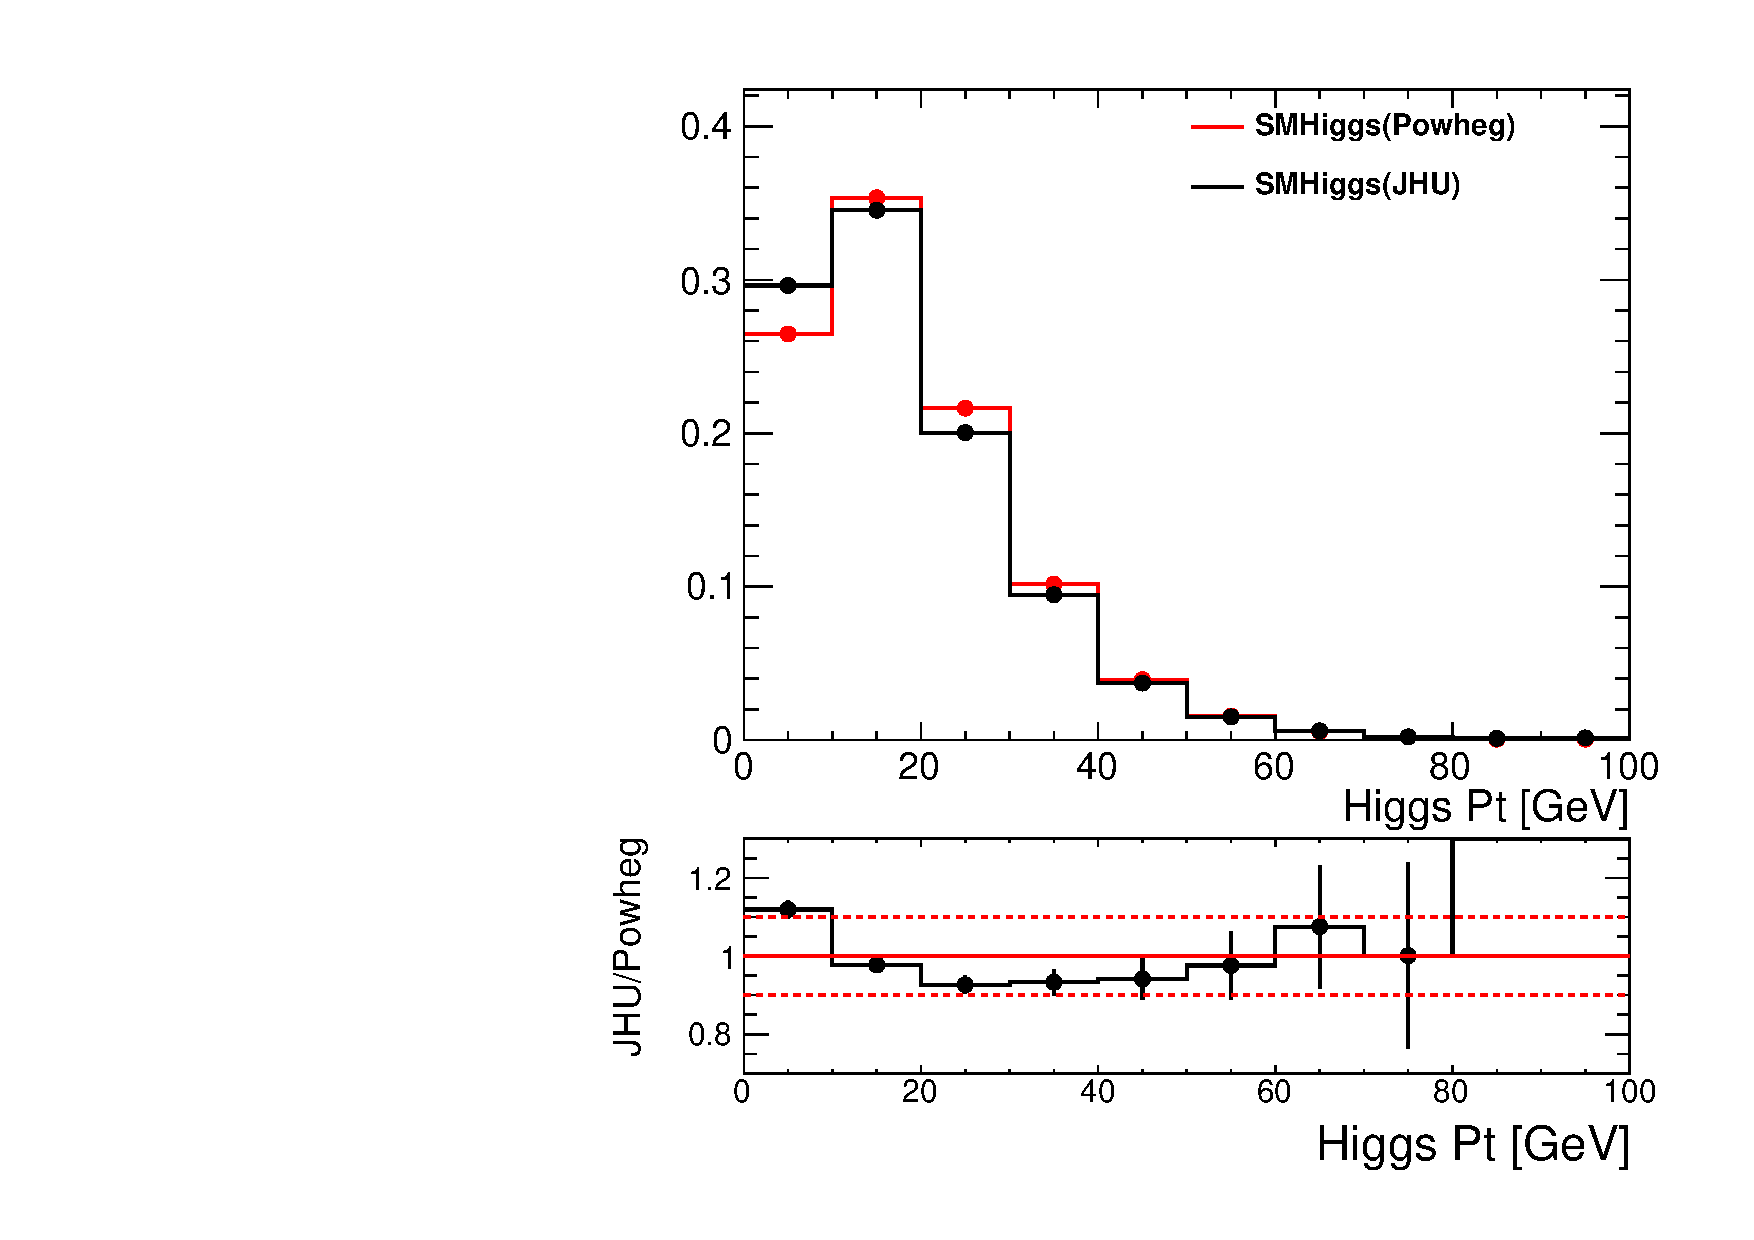
\includegraphics[width=.3\textwidth]{figures/higgsPt.pdf}
}
\subfigure[Leading Jet $\pt$]{
\centering
\label{subfig:jet1pt_0j}
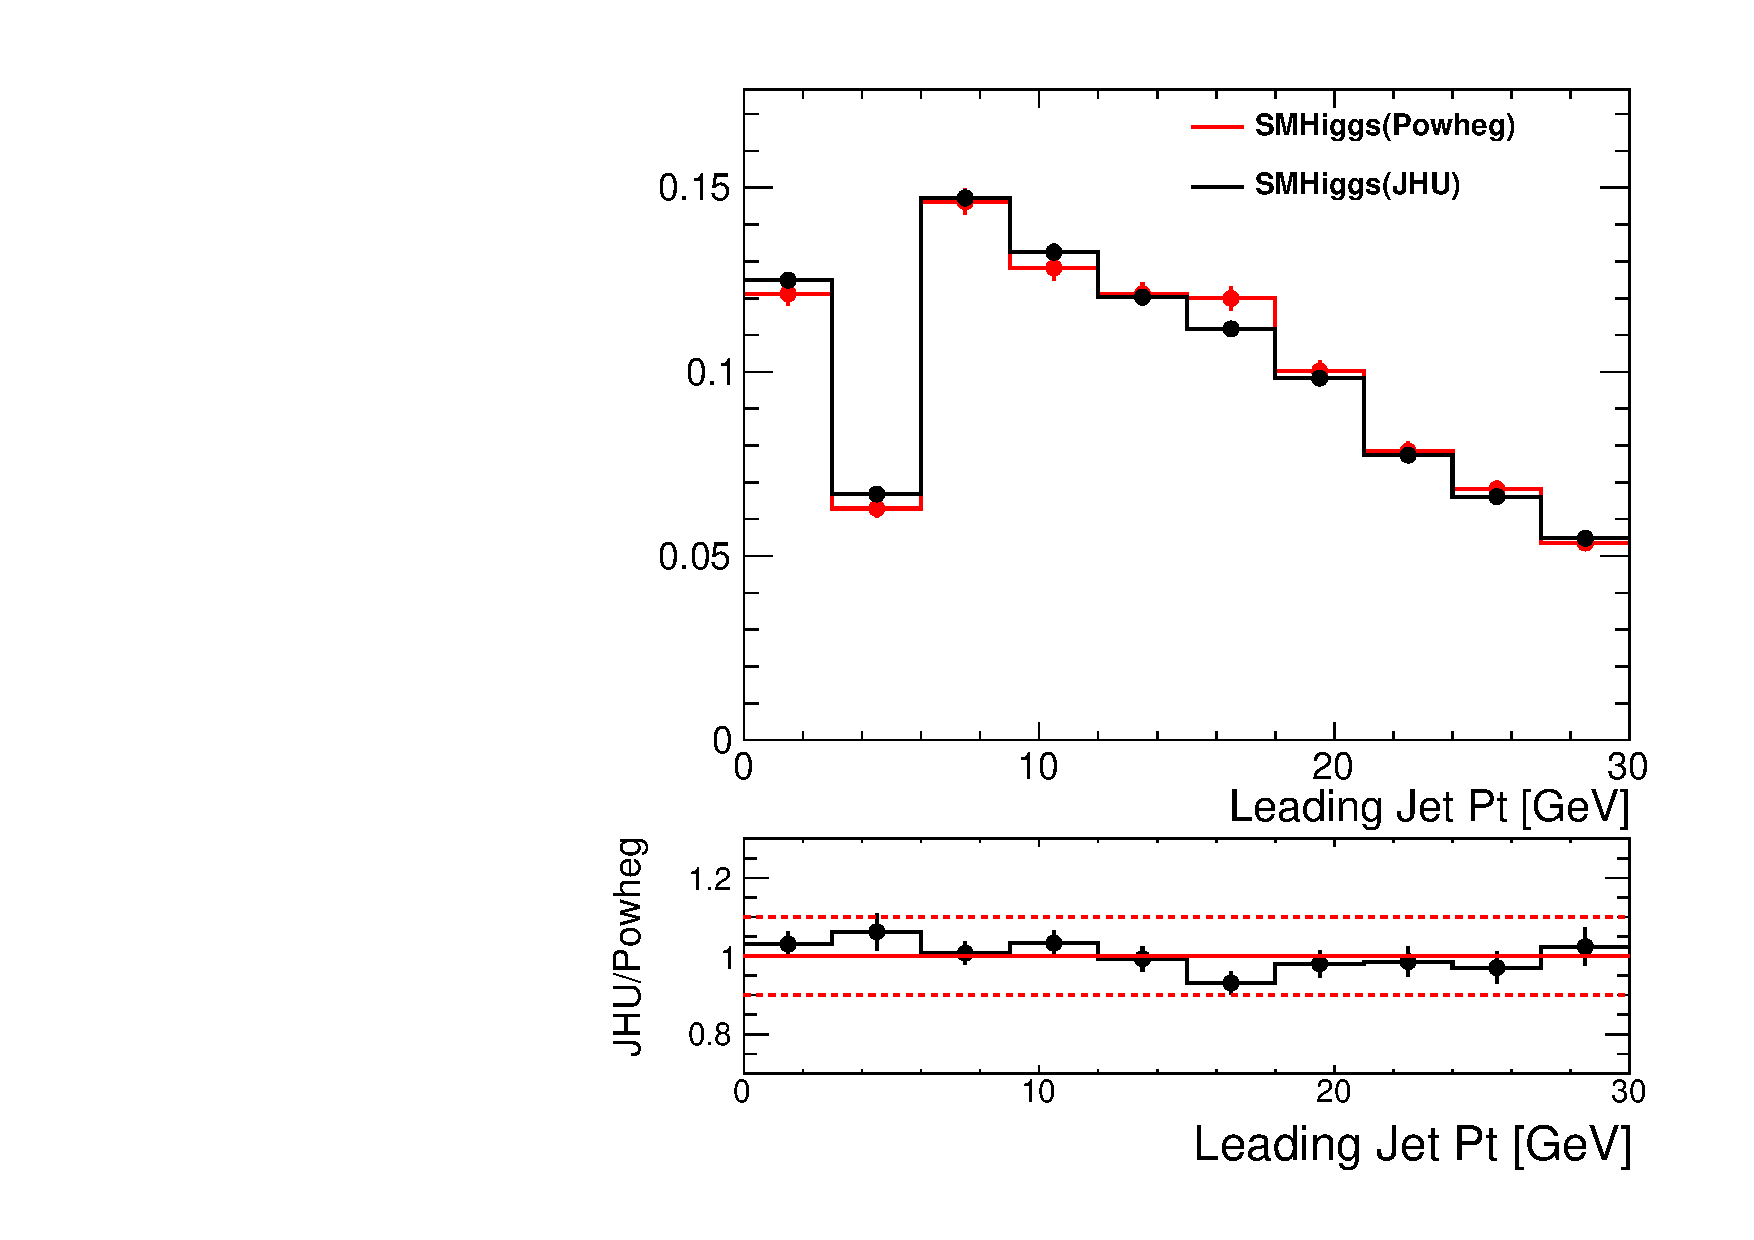
\includegraphics[width=.3\textwidth]{figures/jet1pt.pdf}
}\\
\caption{The Higgs $\pt$ and the leading jet $\pt$ distributions (normalized to 1) of the 
SM Higgs hypothesis comparing the powheg generator and JHUGen, after 
applying the final event selections. }
\label{fig:higgspt_0j}
\end{figure}
%%%%%%%%%%%%%%%%%%%%%%%%%%%%%%%%%%%%%%%%%%%%%


%%%%%%%%%%%%%%%%%%%%%%%%%%%%%%%%%%%%%%%%%%%%%
\begin{figure}[!hbtp]
\centering
\subfigure[Leading Lepton $\pt$]{
\centering
\label{subfig:leadleppt}
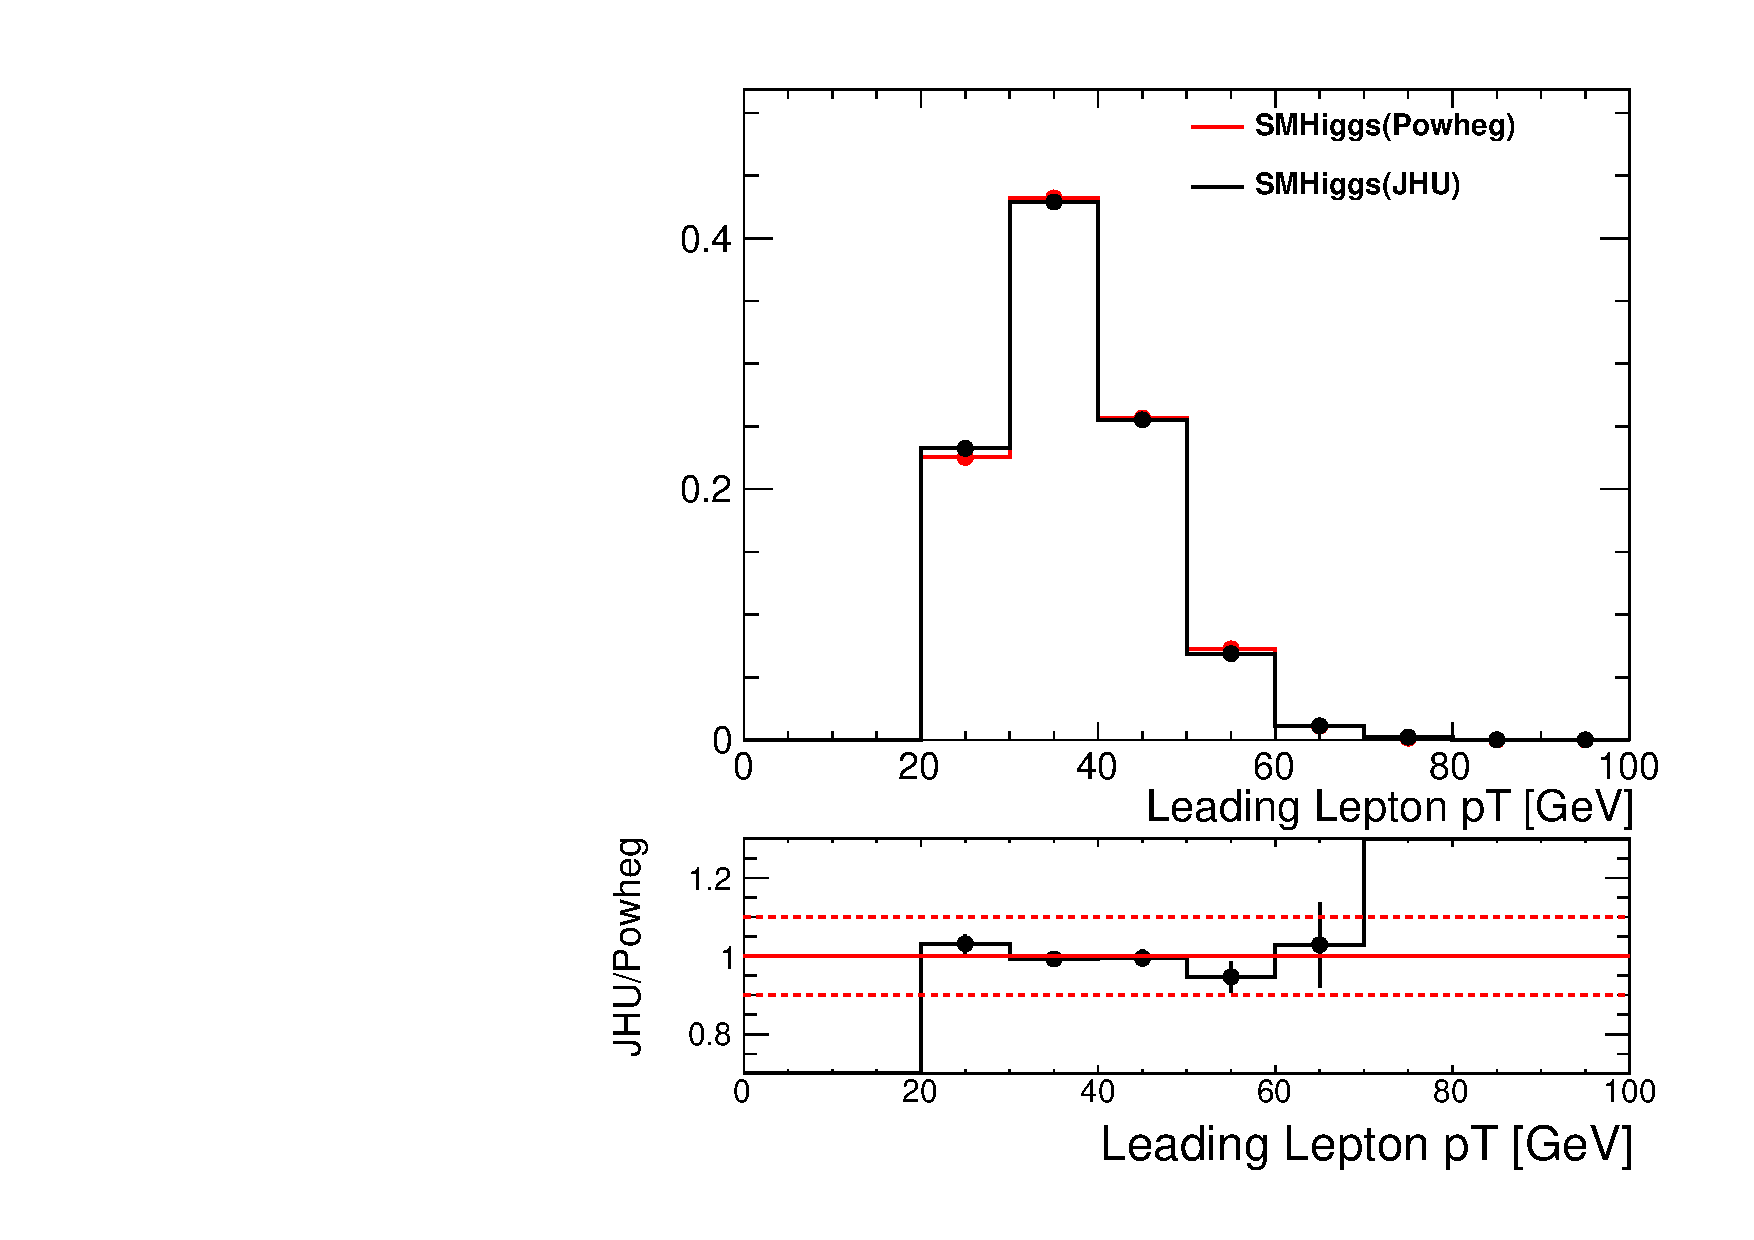
\includegraphics[width=.3\textwidth]{figures/leadleppt.pdf}
}
\subfigure[Trailing Lepton $\pt$]{
\centering
\label{subfig:trailleppt}
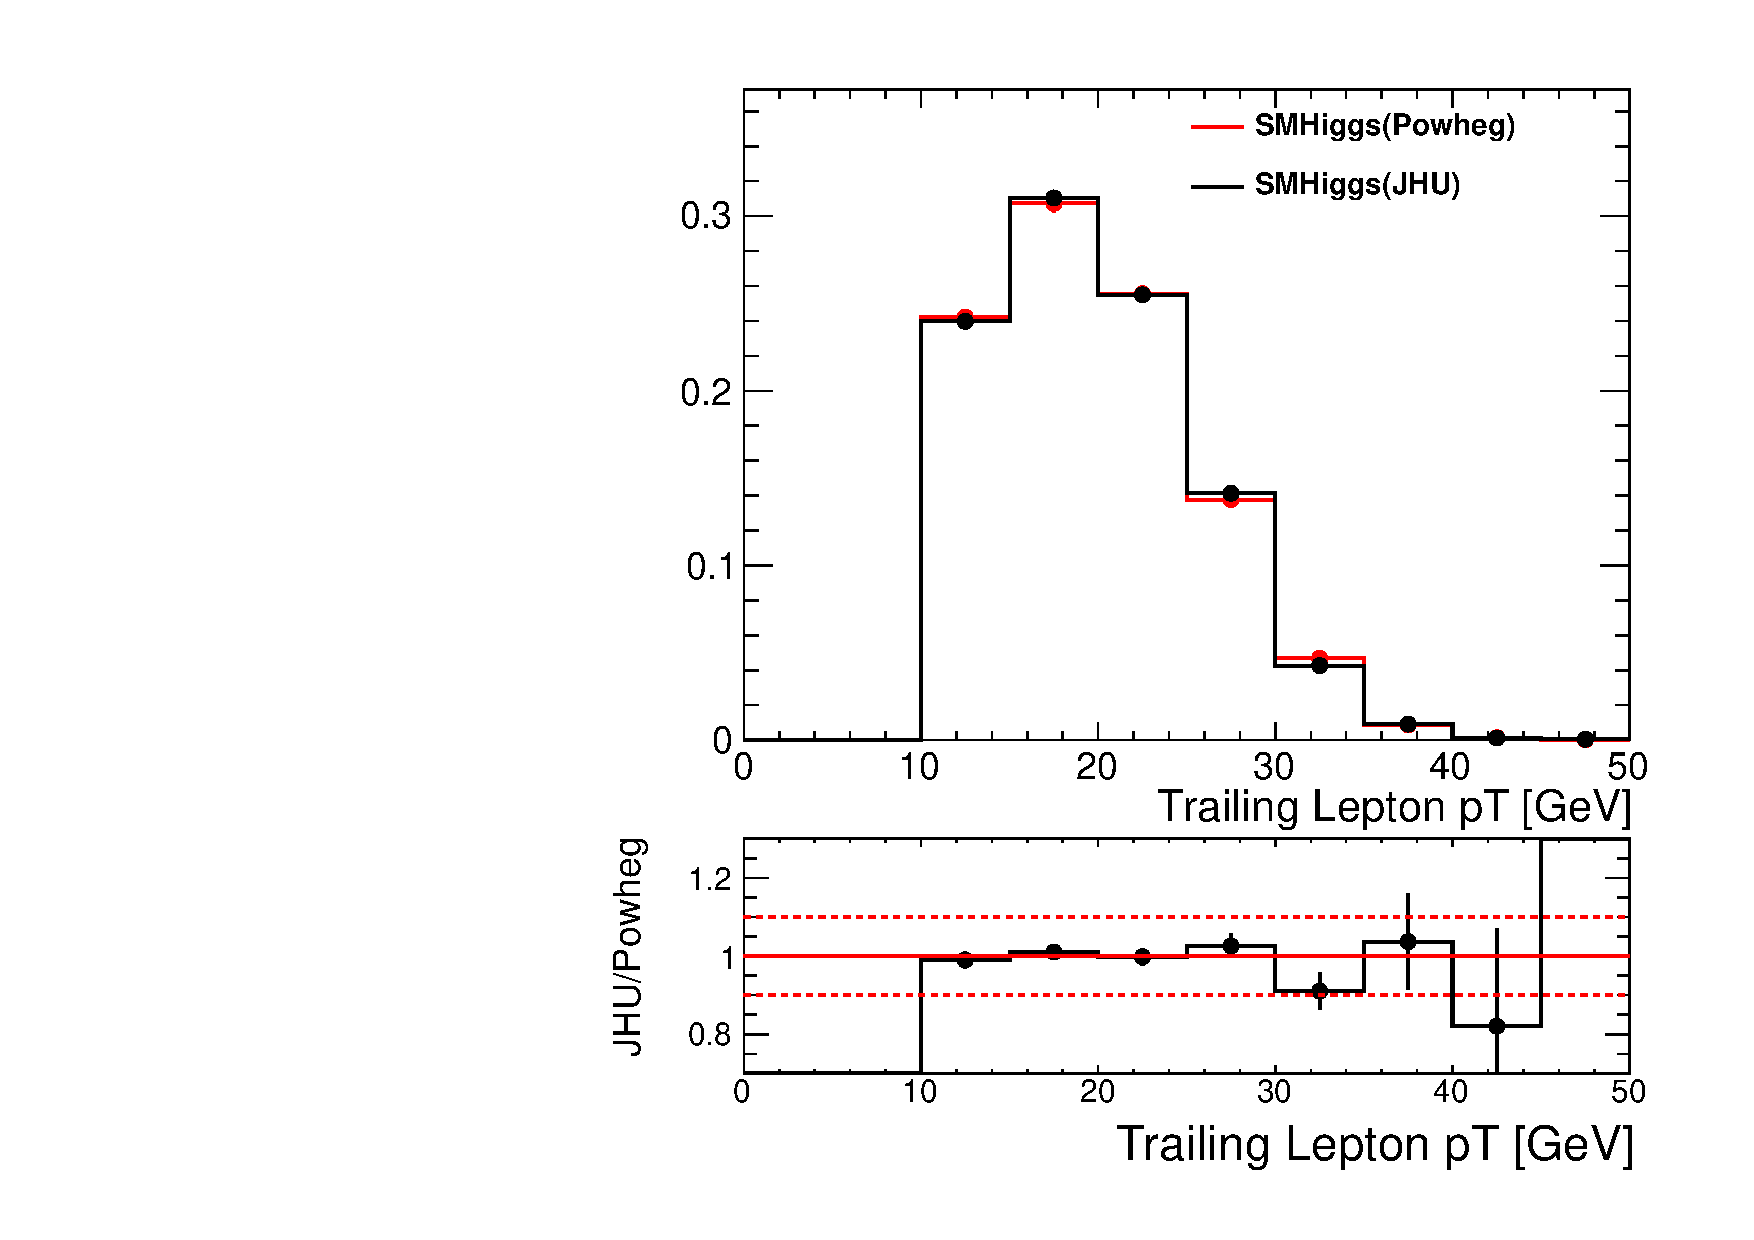
\includegraphics[width=.3\textwidth]{figures/trailleppt.pdf}
}
\subfigure[Leading Lepton $\eta$]{
\centering
\label{subfig:leadlepeta}
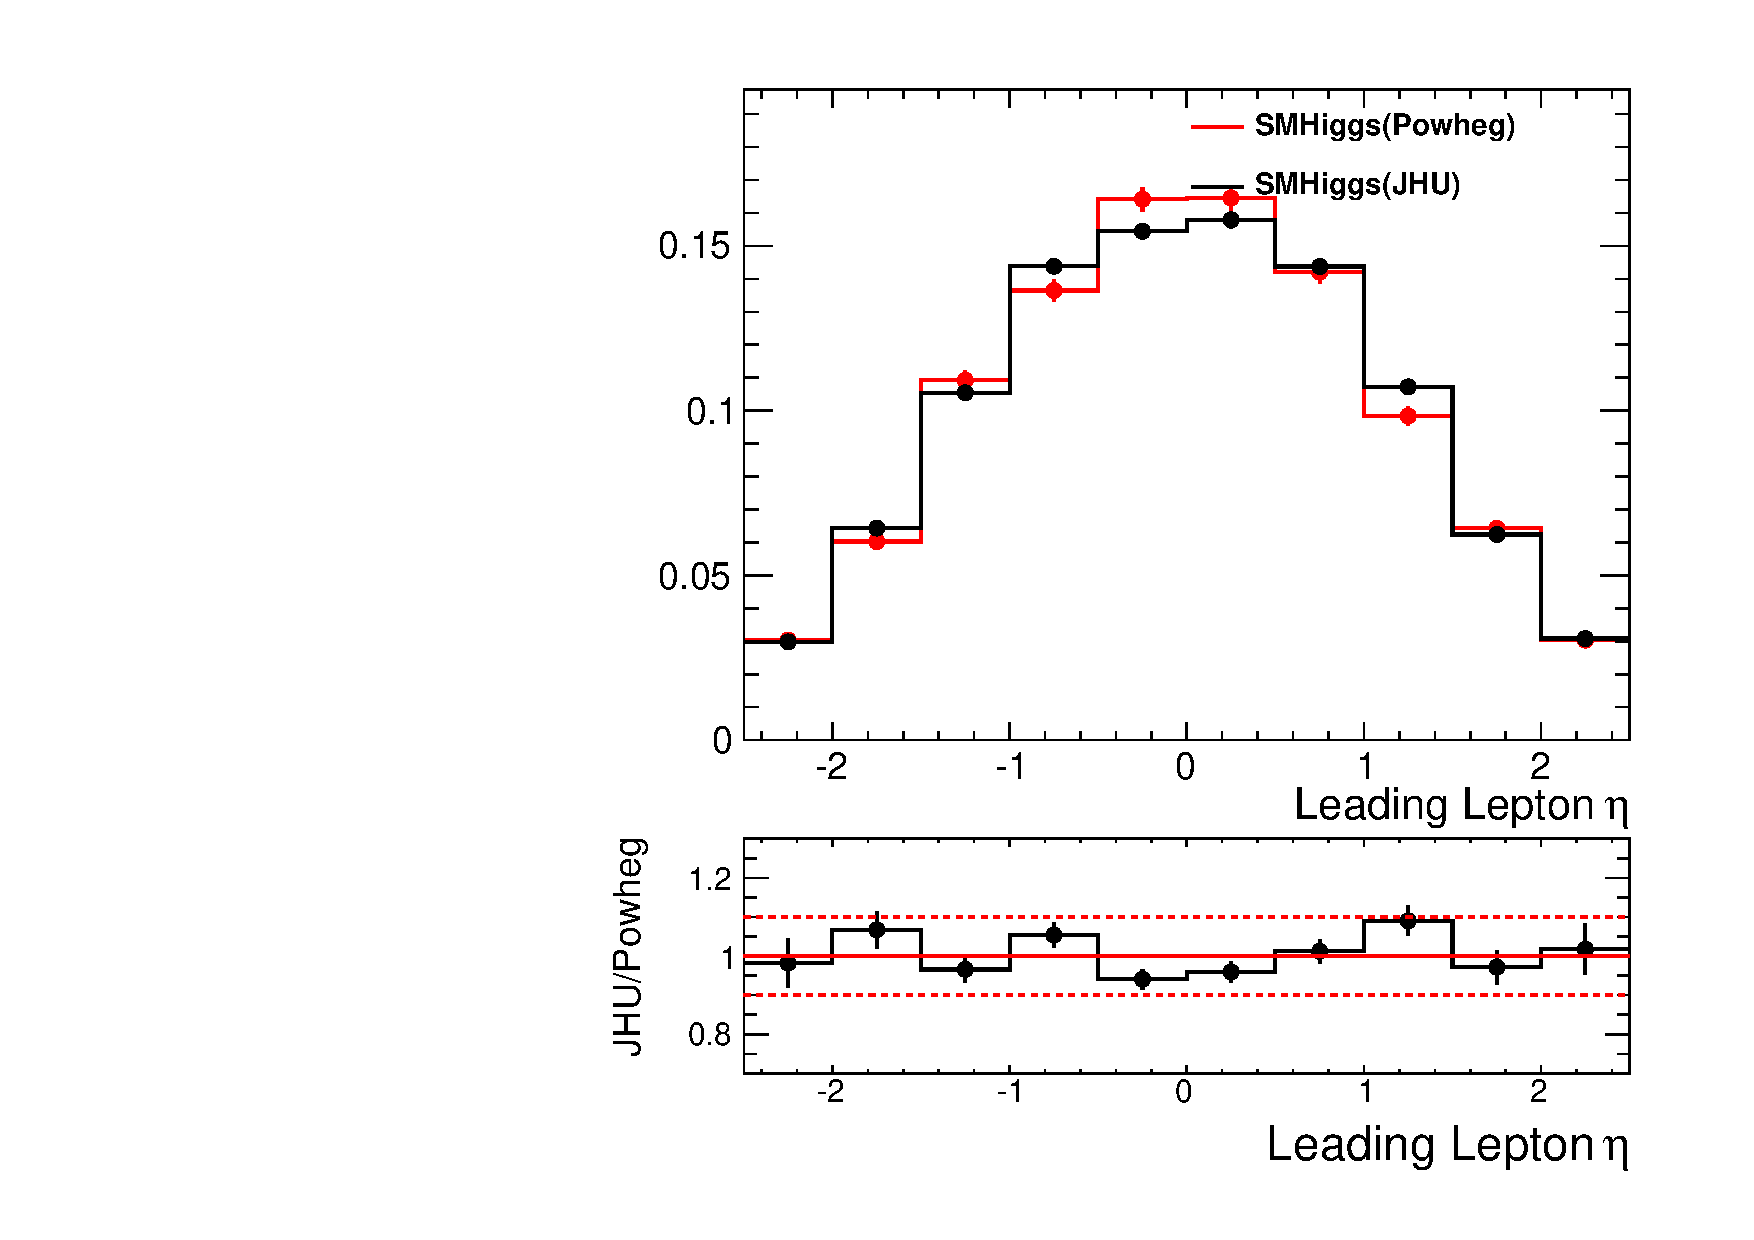
\includegraphics[width=.3\textwidth]{figures/leadlepeta.pdf}
} \\
\subfigure[Trailing Lepton $\eta$]{
\centering
\label{subfig:traillepeta}
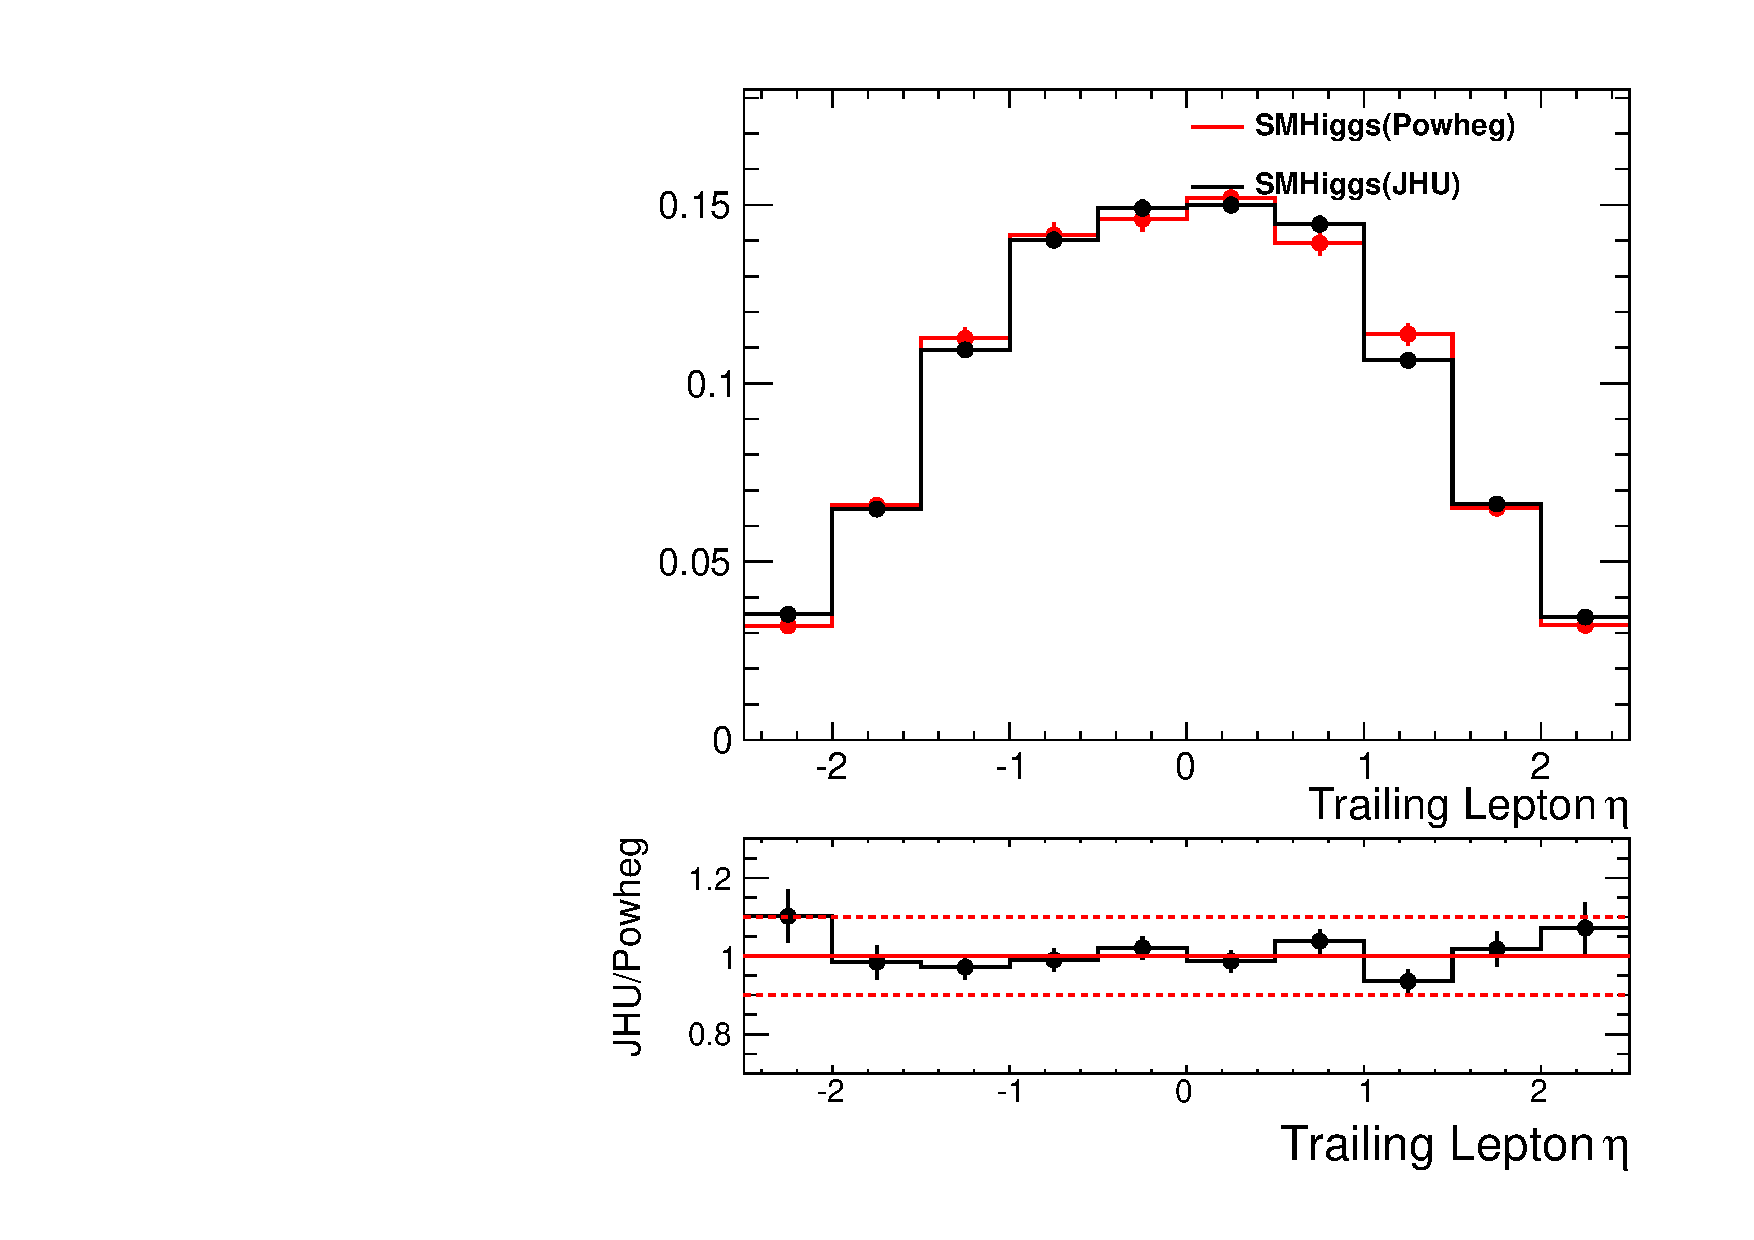
\includegraphics[width=.3\textwidth]{figures/traillepeta.pdf}
}
\subfigure[Dilepton mass]{
\centering
\label{subfig:mll}
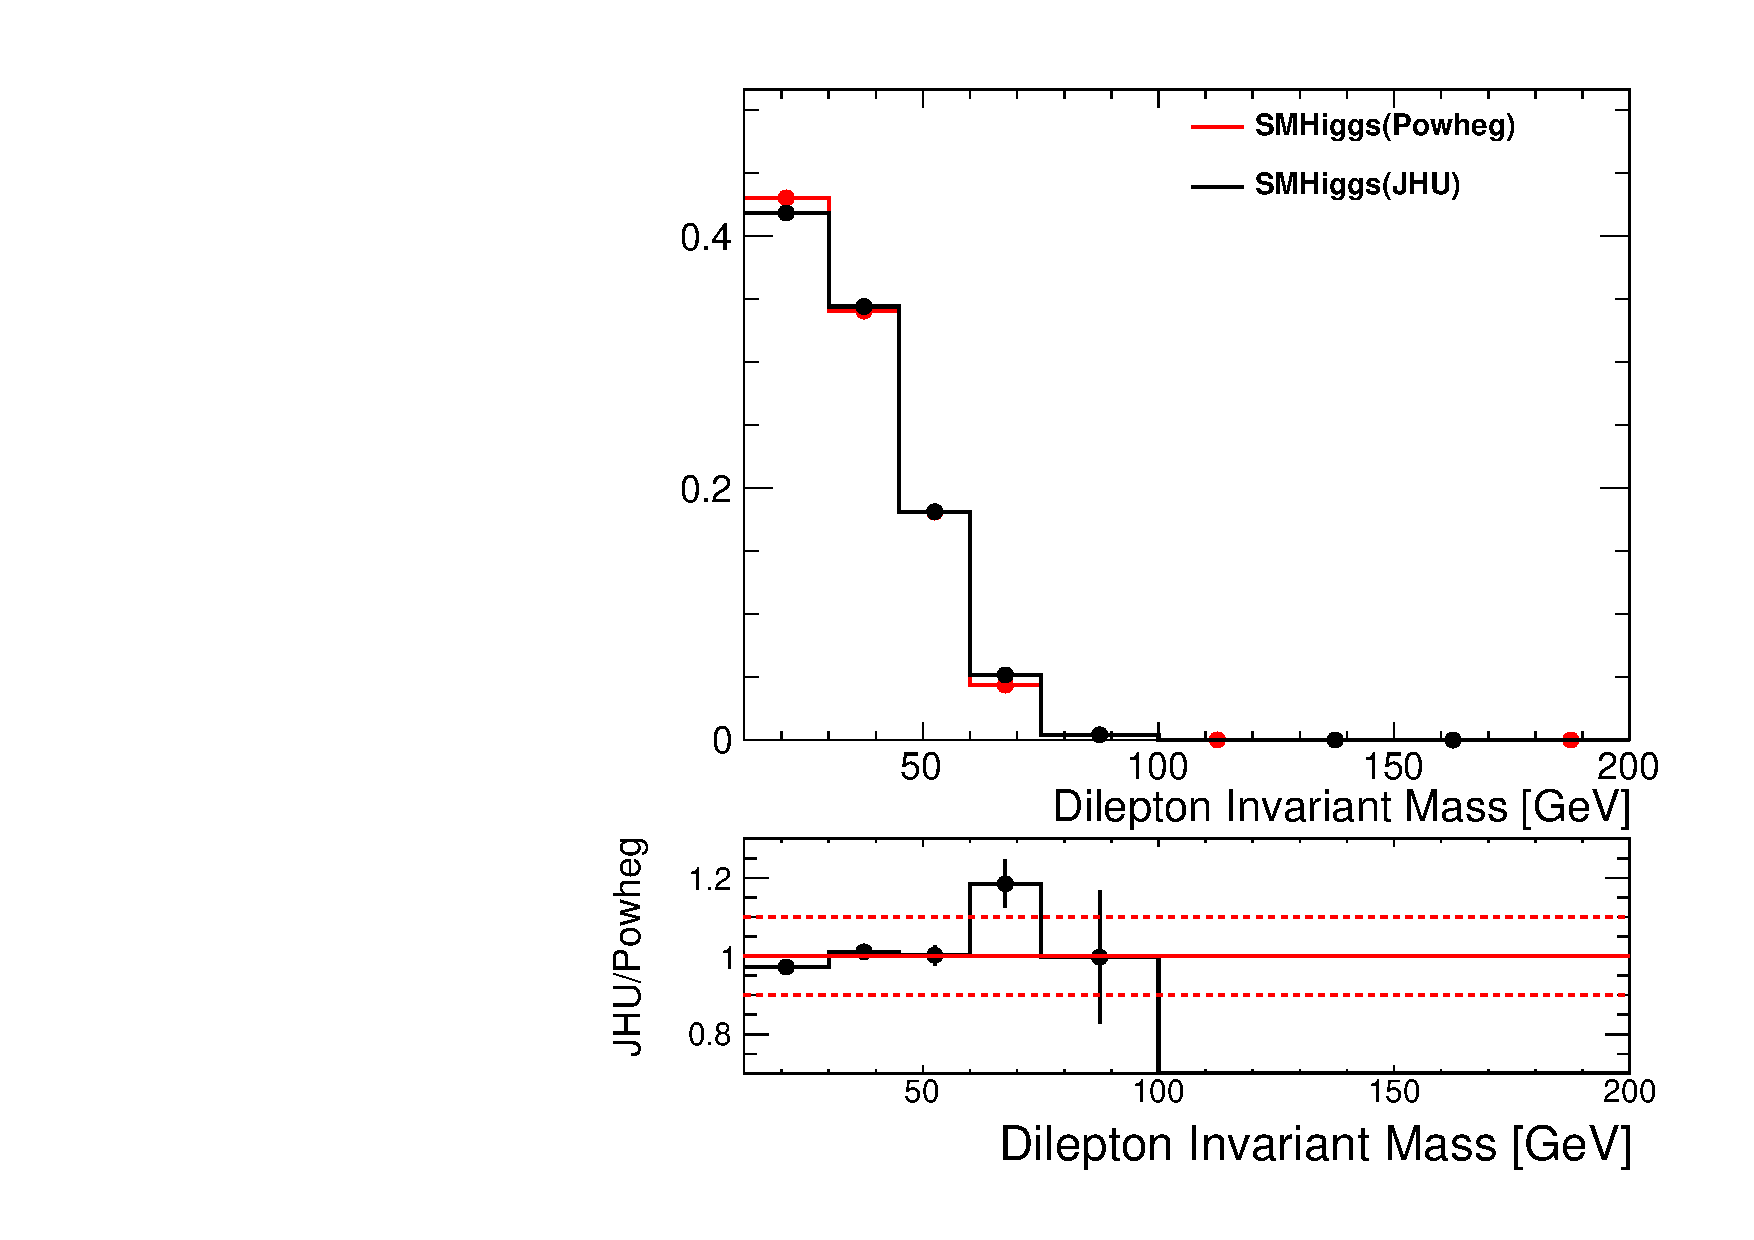
\includegraphics[width=.3\textwidth]{figures/mll.pdf}
} 
\subfigure[Transverse Higgs Mass]{
\centering
\label{subfig:mt}
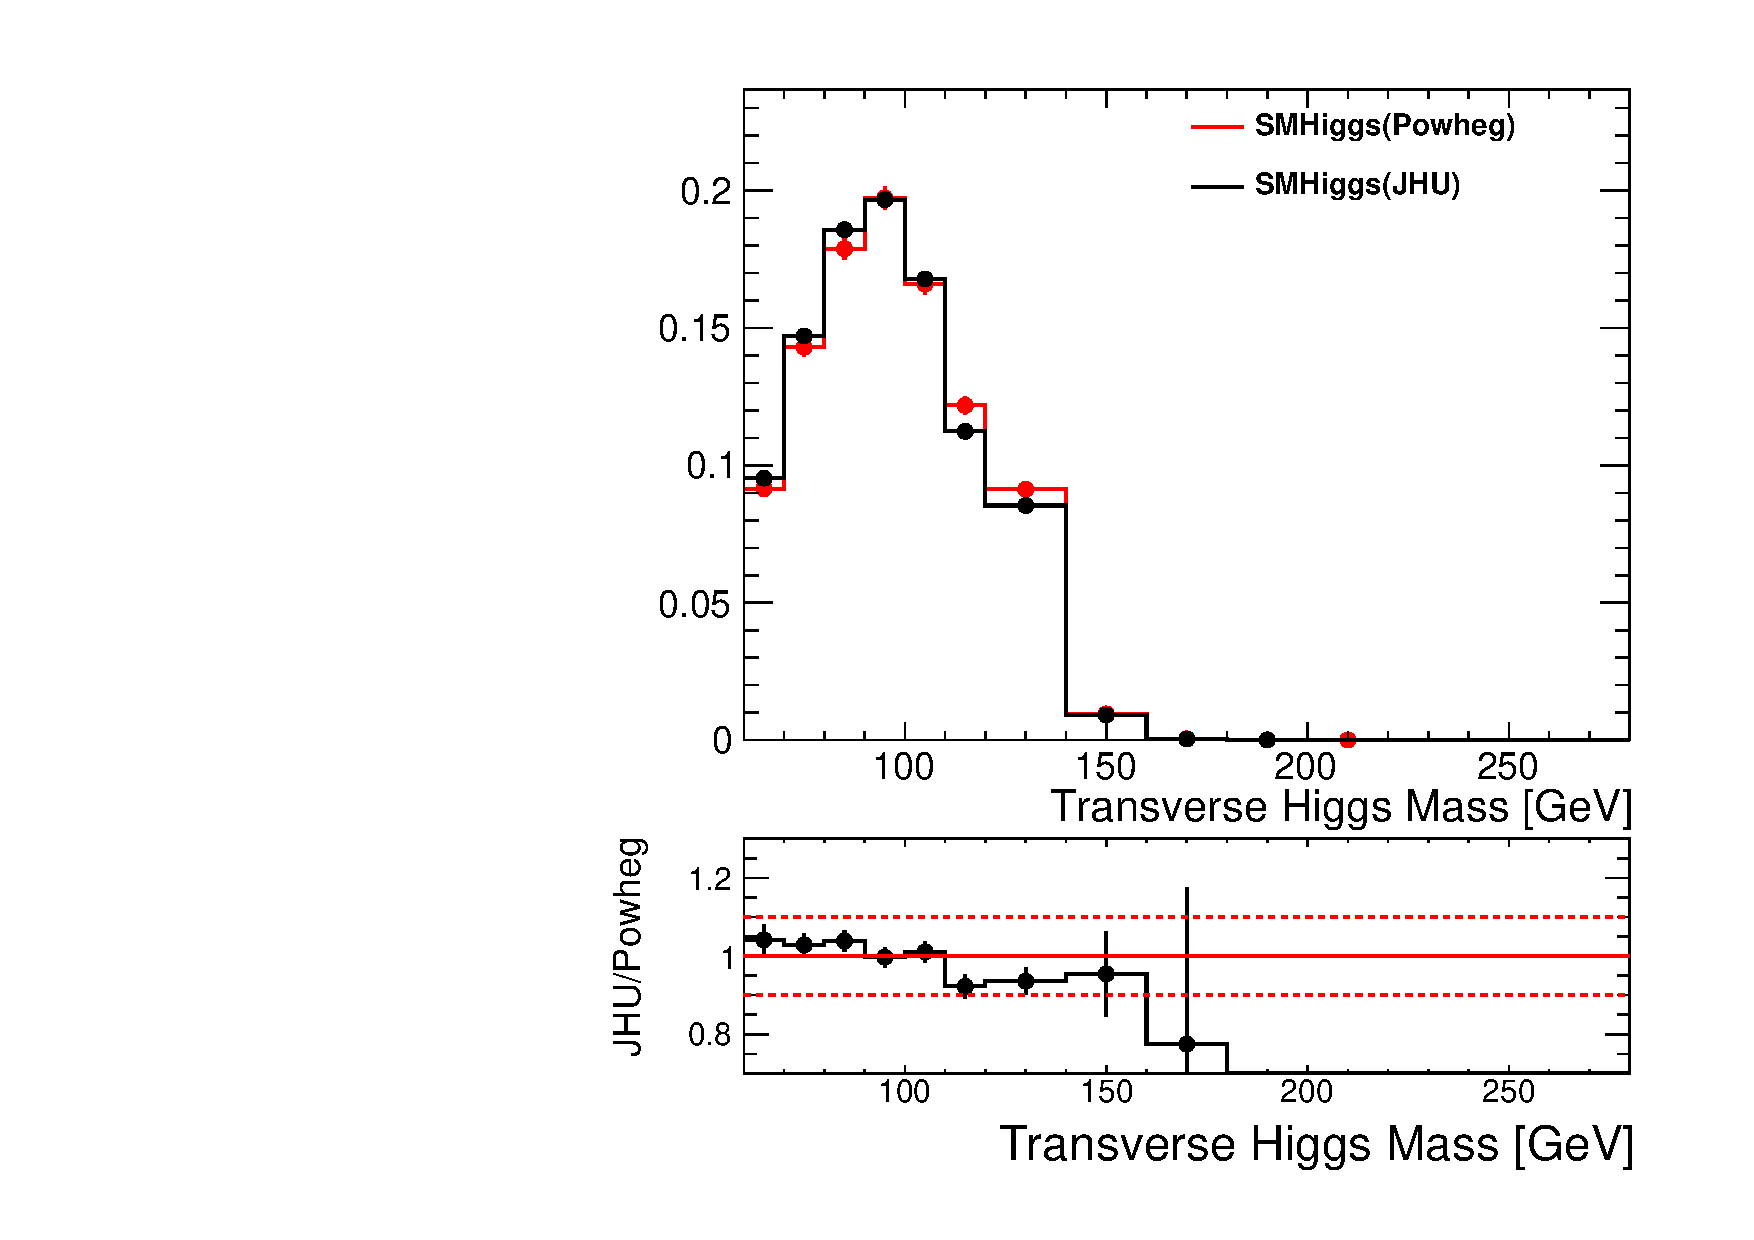
\includegraphics[width=.3\textwidth]{figures/mt.pdf}
}\\
\subfigure[Dilepton $\pt$]{
\centering
\label{subfig:dilpt}
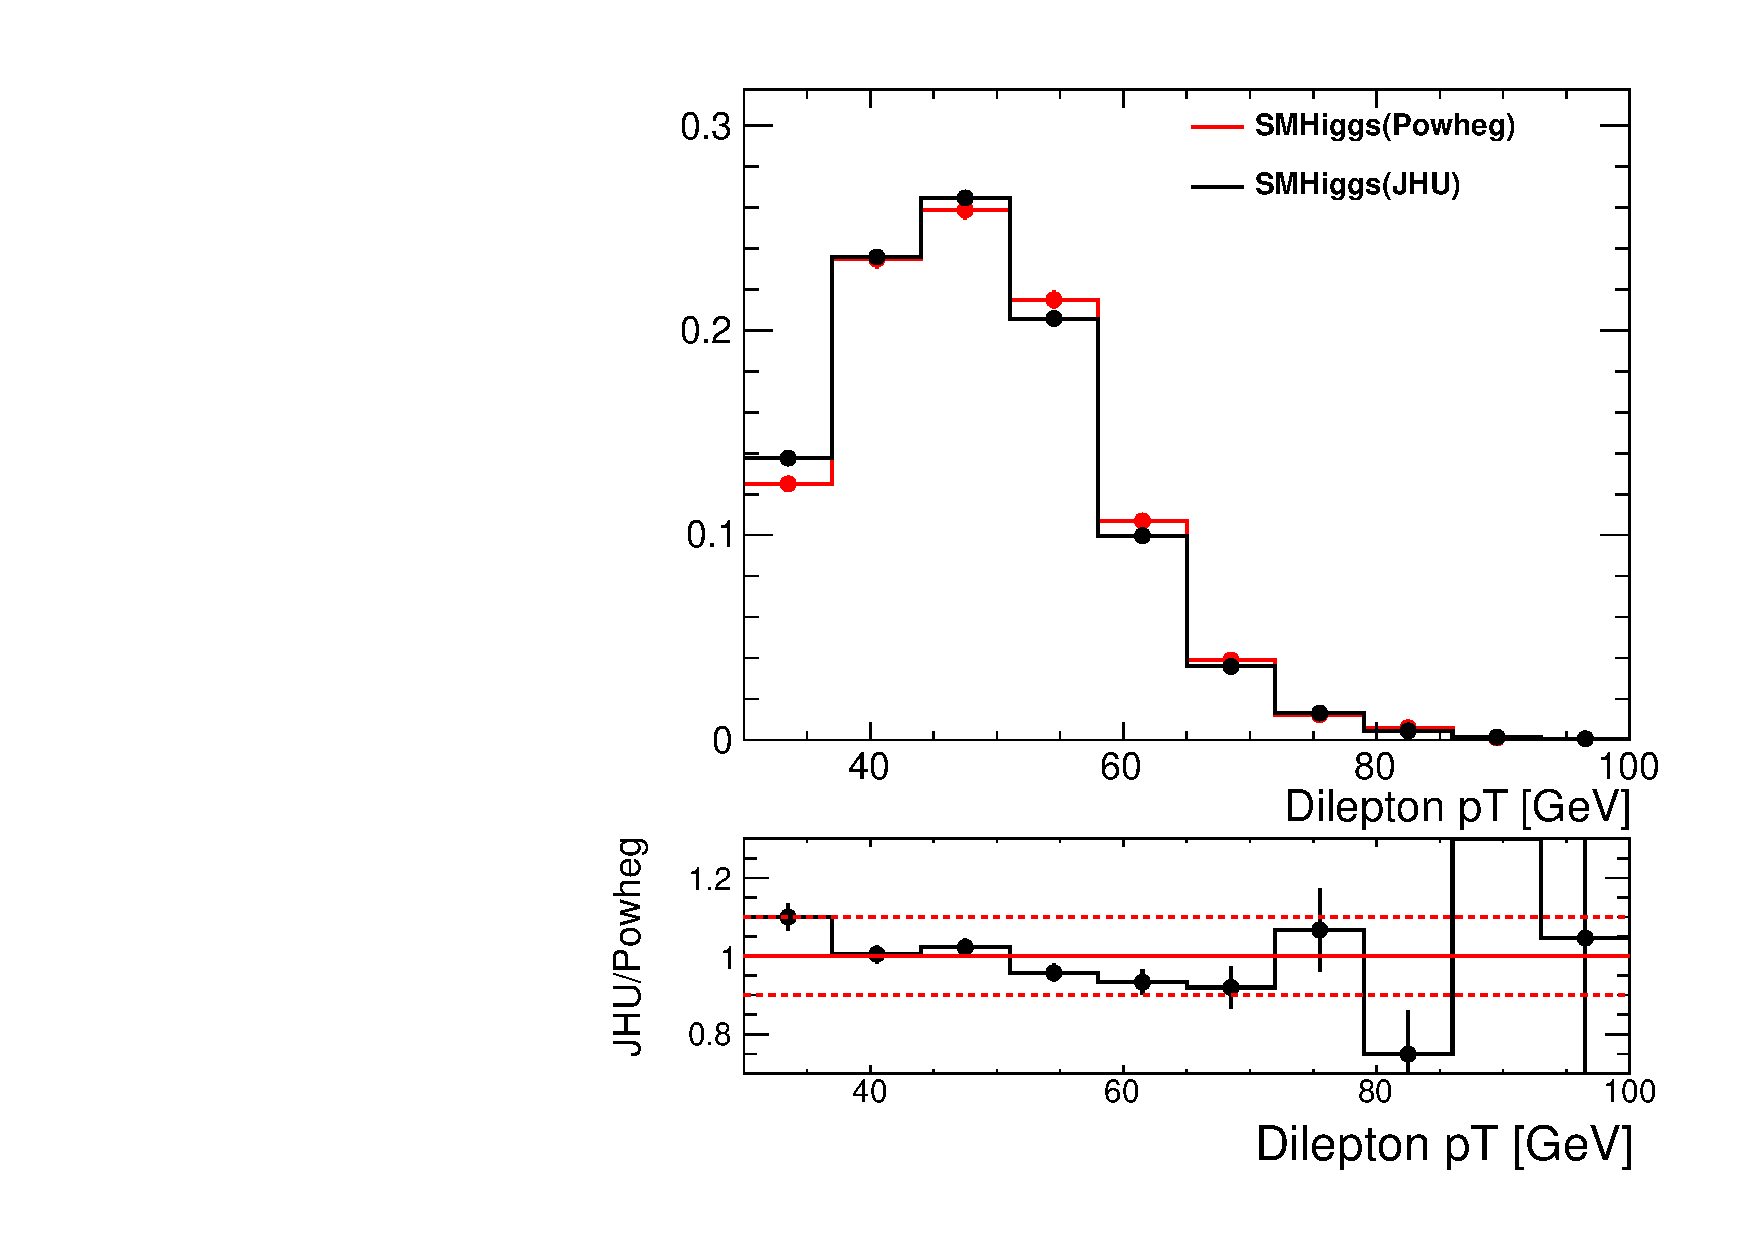
\includegraphics[width=.3\textwidth]{figures/dilpt.pdf}
}
\subfigure[Missing Energy]{
\centering
\label{subfig:met}
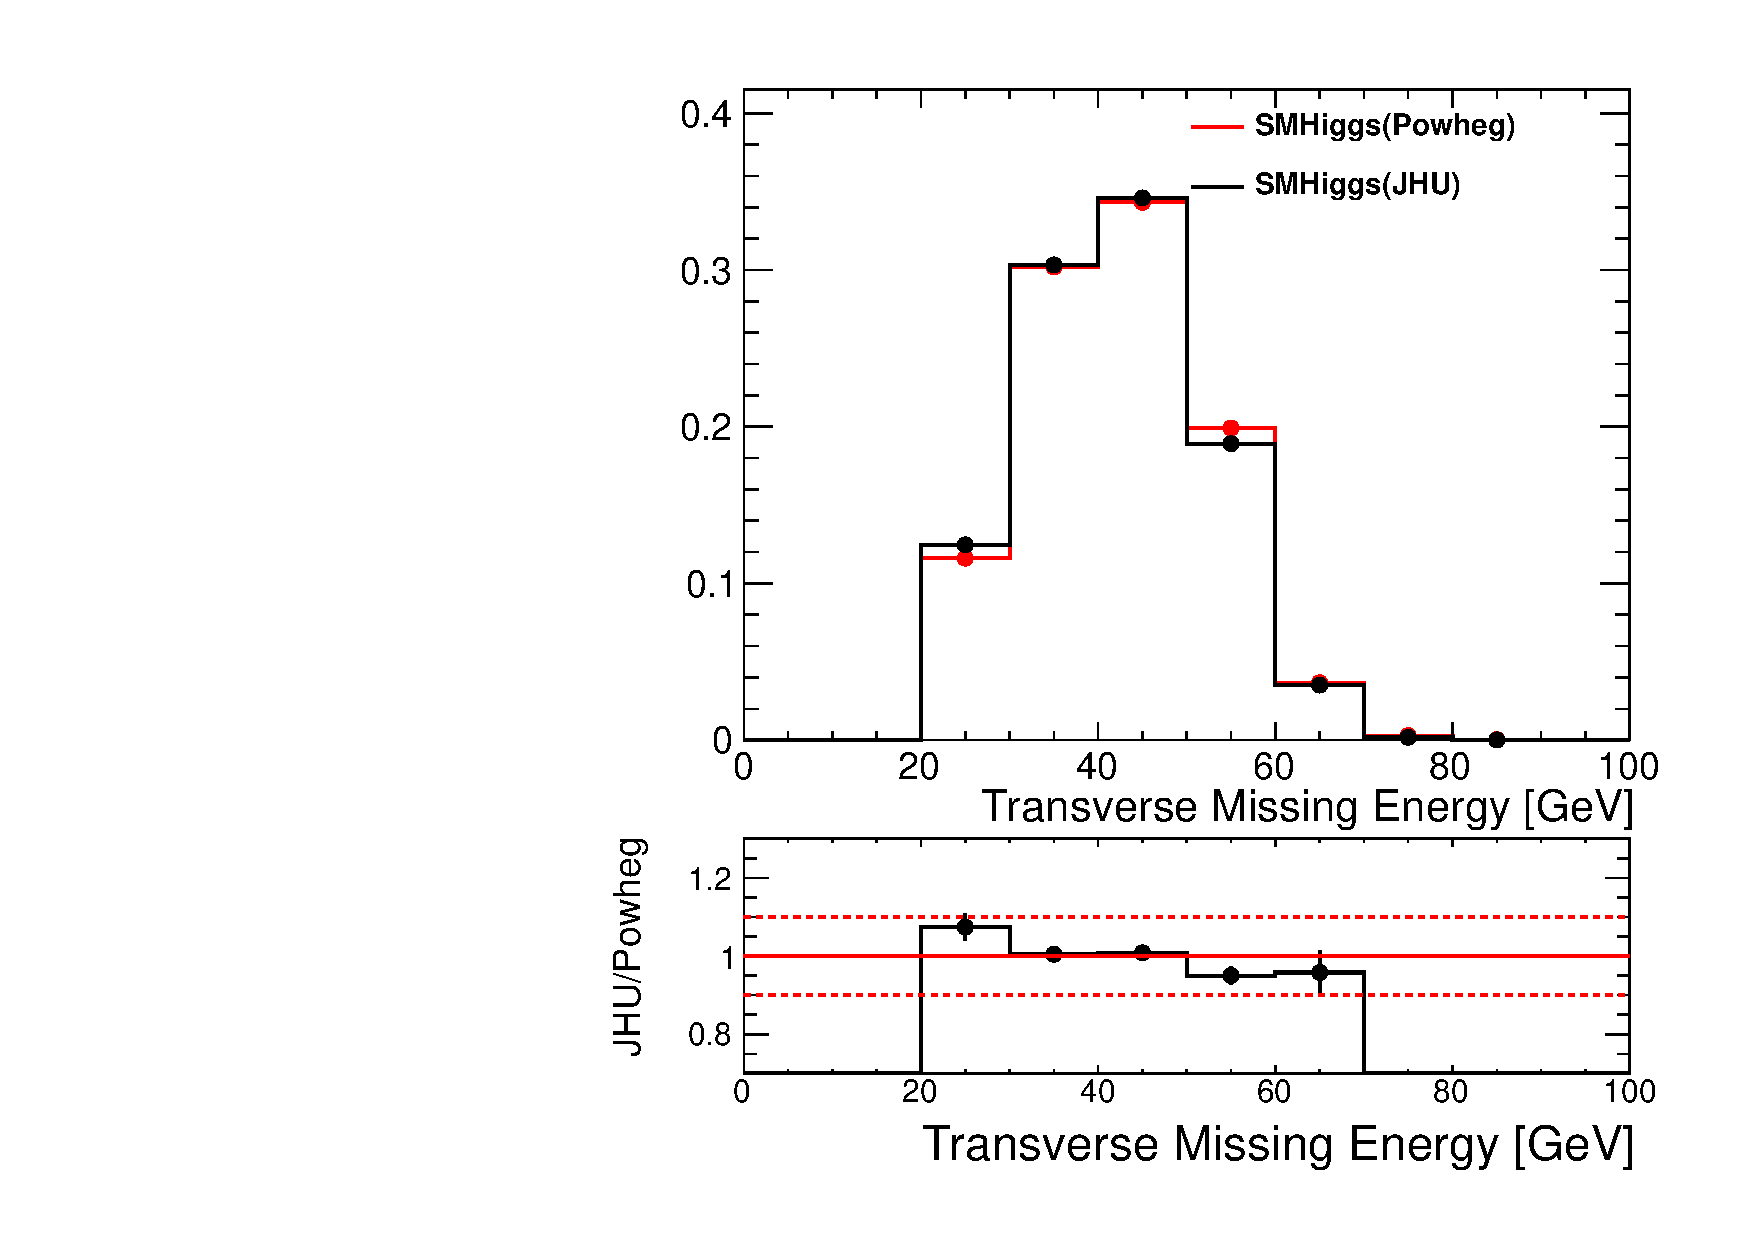
\includegraphics[width=.3\textwidth]{figures/met.pdf}
}
\subfigure[$\Delta\phi_{\ell\ell}$]{
\centering
\label{subfig:met}
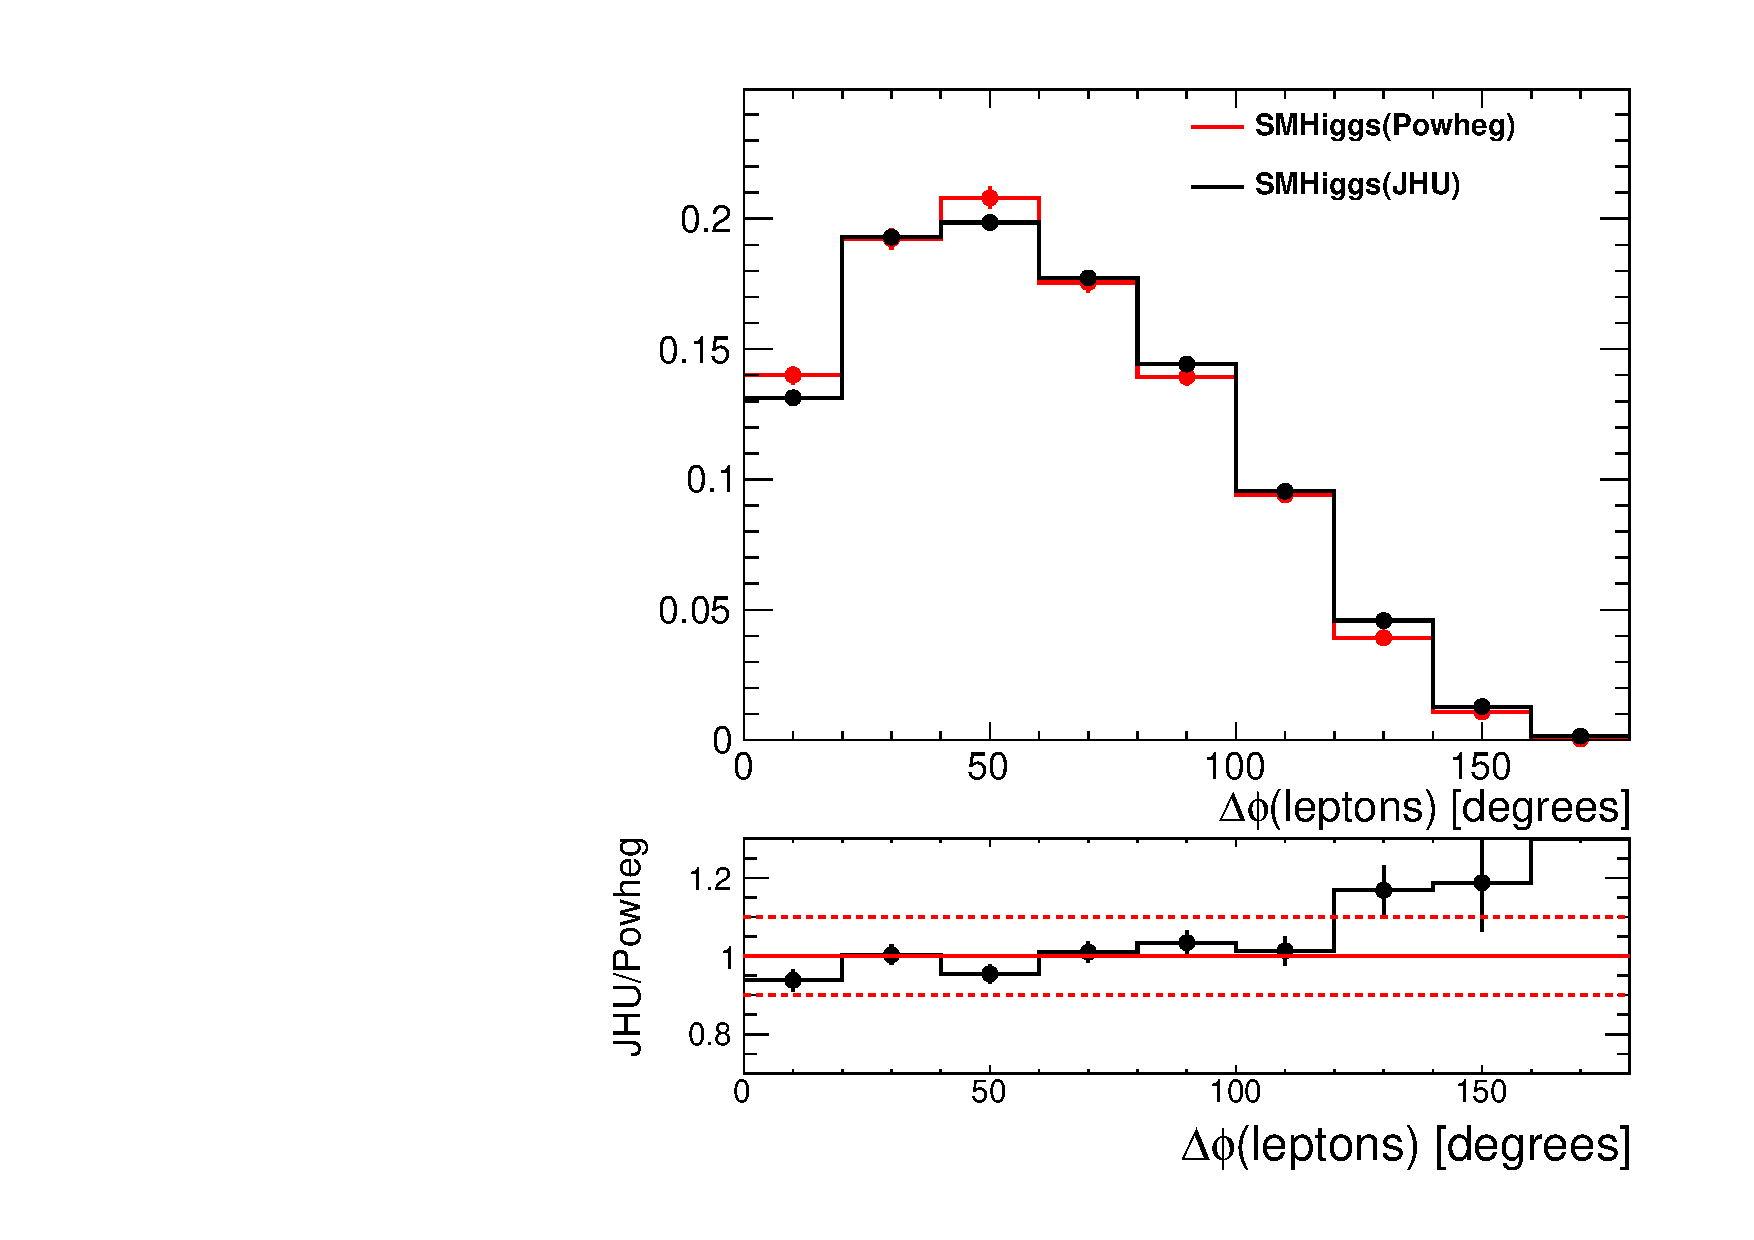
\includegraphics[width=.3\textwidth]{figures/dphill.pdf}
}\\
\caption{Kinematic distributions (normalized to 1) of the SM Higgs hypothesis 
comparing Powheg-Pythia and JHUGen-Pythia for reconstructed events 
after final event selections. }
\label{fig:higgskin_0j}
\end{figure}
%%%%%%%%%%%%%%%%%%%%%%%%%%%%%%%%%%%%%%%%%%%%%

%%%%%%%%%%%%%%%%%%%%%%%%%%%%%%%%%%%%%%%%%%%%%
\begin{figure}[!hbtp]
\centering
\subfigure[Higgs $\pt$]{
\centering
\label{subfig:higgspt_0j}
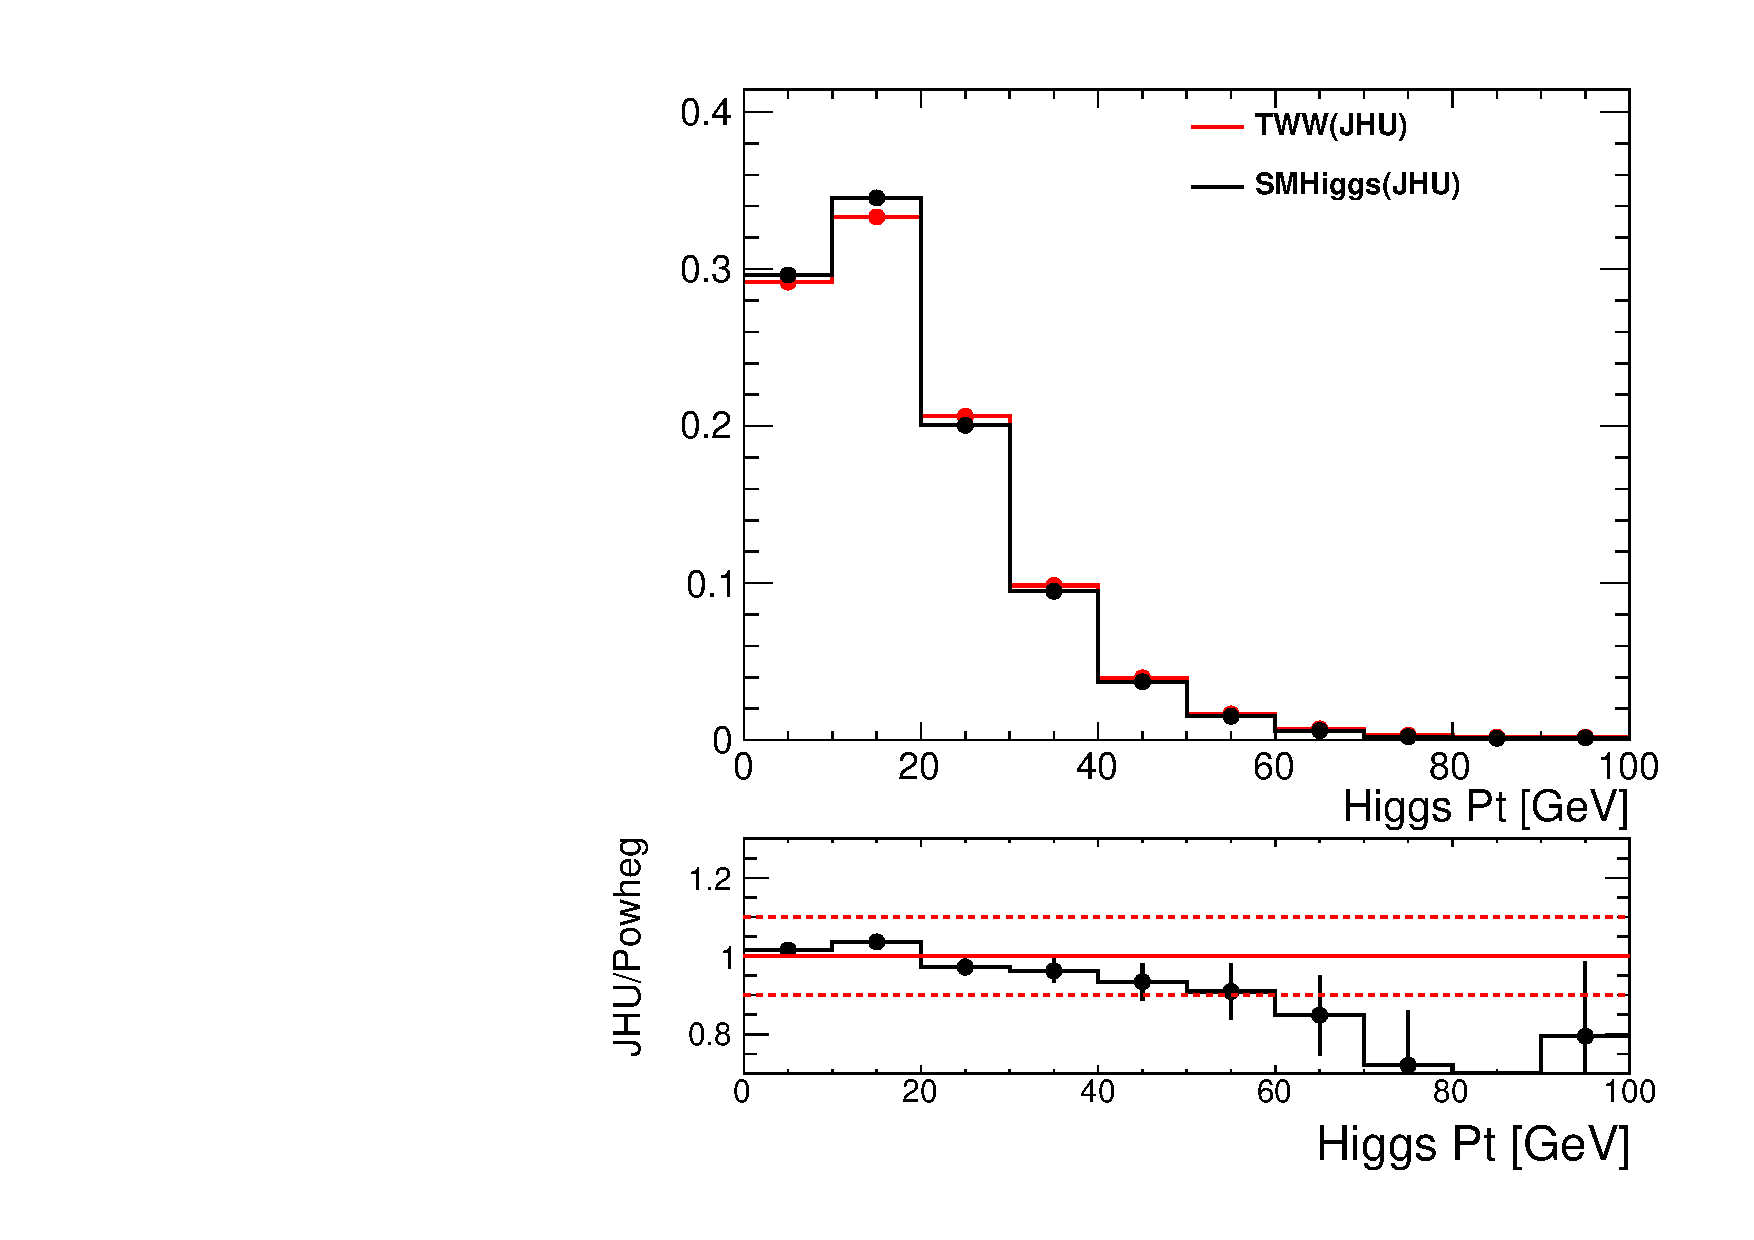
\includegraphics[width=.3\textwidth]{figures/higgsPt_gravitonvshiggs.pdf}
}
\subfigure[Leading Jet $\pt$]{
\centering
\label{subfig:jet1pt_0j}
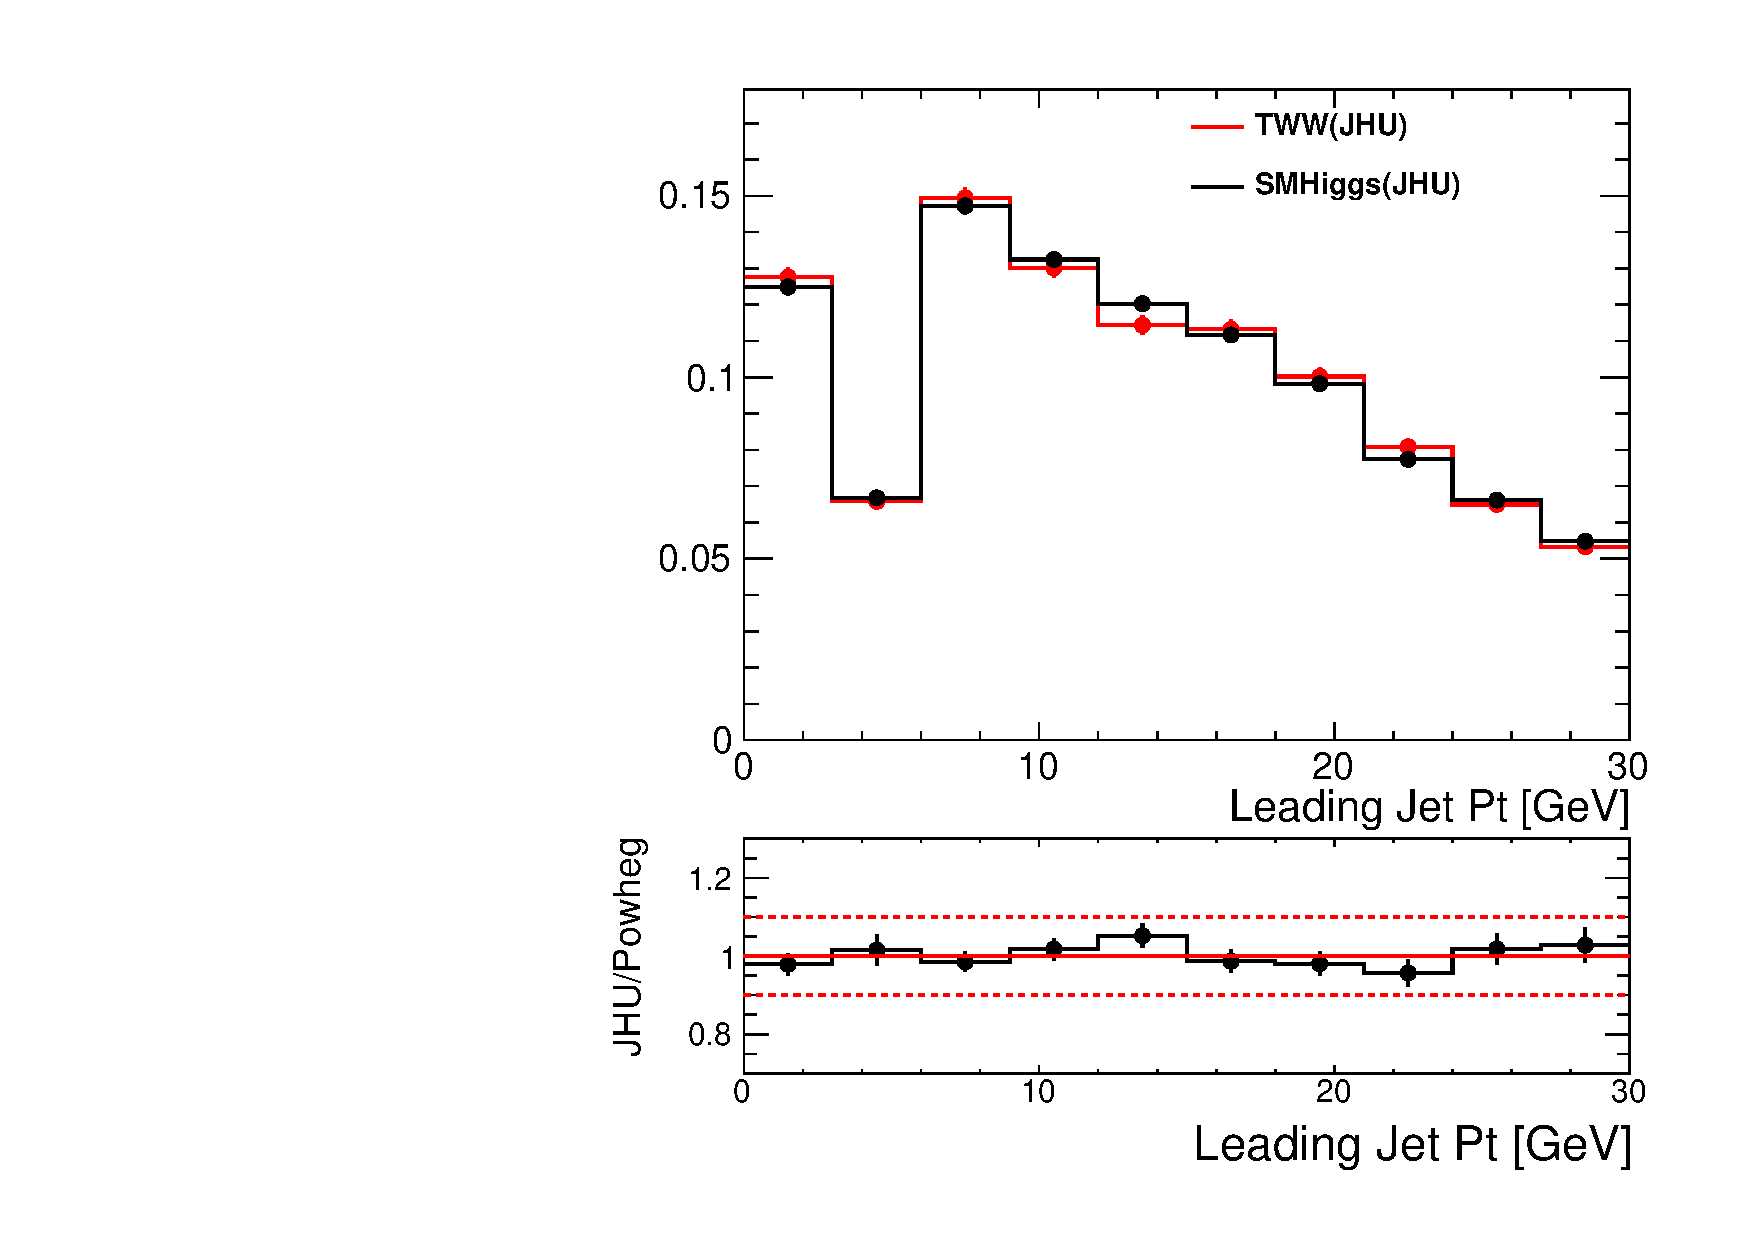
\includegraphics[width=.3\textwidth]{figures/jet1pt_gravitonvshiggs.pdf}
}\\
\caption{The Higgs $\pt$ and the leading jet $\pt$ distributions (normalized to 1) of the 
SM Higgs hypothesis compared to the Graviton ($2_\text{min}^+$) hypothesis, applying 
final event selections. }
\label{fig:gravvshiggspt_0j}
\end{figure}
%%%%%%%%%%%%%%%%%%%%%%%%%%%%%%%%%%%%%%%%%%%%%


\clearpage

\section{Signal Extraction Strategy}
\label{sec:sigextract}
We use the same event selections as in the SM Higgs search 
~\cite{HWWHCP2012} with the exception of two changes.
To improve the selection efficiency for the $gg\to X\to WW$ hypothesis,
we apply dilepton $p_T>$ 30 GeV and transverse mass $m_T>$60 GeV.
To improve the signal purity we use events in the 0-Jet bin 
and only consider the different lepton flavor final state.

We analyse the data by constructing two dimensional templates based on $m_T-m_{\ell\ell}$.
This is the same procedure used in the SM Higgs search.
In this analysis, the templates defined as follows:

%%%%%%%%%%%%%%%%%
\begin{itemize}
\item $m_T$ 14 bins: [60,70,80,90,100,110,120,140,160,180,200,220,240,260,280],
\item $m_{\ell\ell}$ bins: [12,30,45,60,75,100,125,150,175,200].
\end{itemize}
%%%%%%%%%%%%%%%%%

This template binning is chosen to ensure the following conditions are met:

%%%%%%%%%%%%%%%%%
\begin{itemize}
    \item enough statistics for the main signal and background processes, 
    \item enough granuarity in the signal enriched regions to distinguish between 
different hypotheses, 
    \item the same binning in the background enriched (mainly $WW$ and $Top$) regions 
as in the SM Higgs search~\cite{HWWHCP2012}. 
\end{itemize}
%%%%%%%%%%%%%%%%%

The $m_T-m_{\ell\ell}$ templates for the SM Higgs boson and 
the spin-2 graviton like resonance $2_\text{min}^+$, zoomed in the 
signal enriched regions, are shown normalised to \intlumiEightTeV 
in Figure~\ref{fig:mtvsmll_sig}.
The corresponding background temlates are shown in 
Figure~\ref{fig:mtvsmll_bkg}, and the expected signal and
background yields for \intlumiEightTeV are shown in Table~\ref{tab:yield}.

To separate the standard model and $gg\to X\to WW$ hypotheses,
we construct a signal plus background model for each hypothesis.
The same event selections and background predictions are used for both models.
We then perform the CLs fit for both models to the data, letting the 
signal strength float.
The difference in the best fit likelihoods is then used 
to quantify the consistency between data and each signal hypothesis. 

To calculate the expected separation between the SM Higgs and other 
exotic resonances, we use the same number of events for the exotic resonance
after the full selections as in the SM Higgs case. 

%%%%%%%%%%%%%%%%%%%%%%%%%%%%%%%%%%%%%%%%%%%%%
\begin{figure}[!hbtp]
\centering
\subfigure[SM Higgs]{
\centering
\label{subfig:hww}
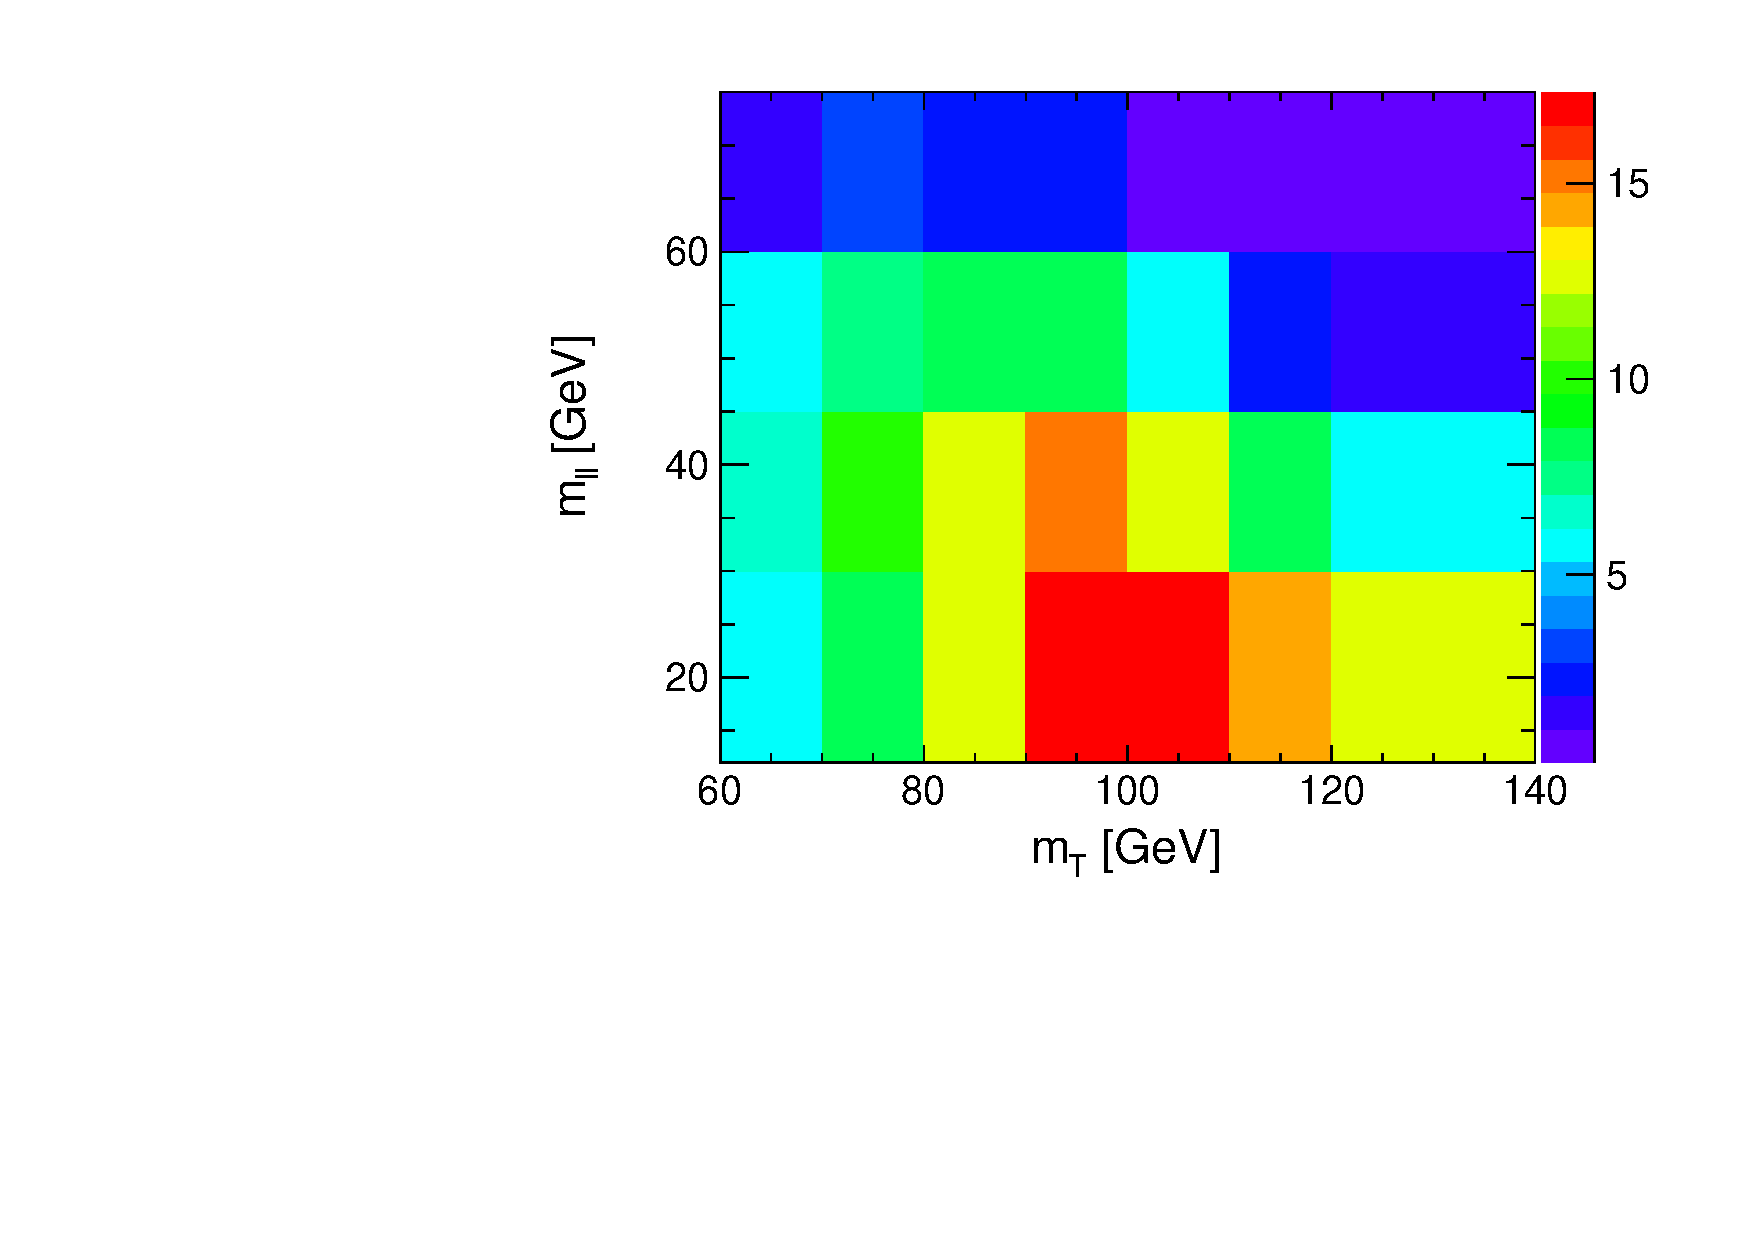
\includegraphics[width=.45\textwidth]{figures/mtvsmll_hww.pdf}
}
\subfigure[Graviton ($2_m^+$)]{
\centering
\label{subfig:xww}
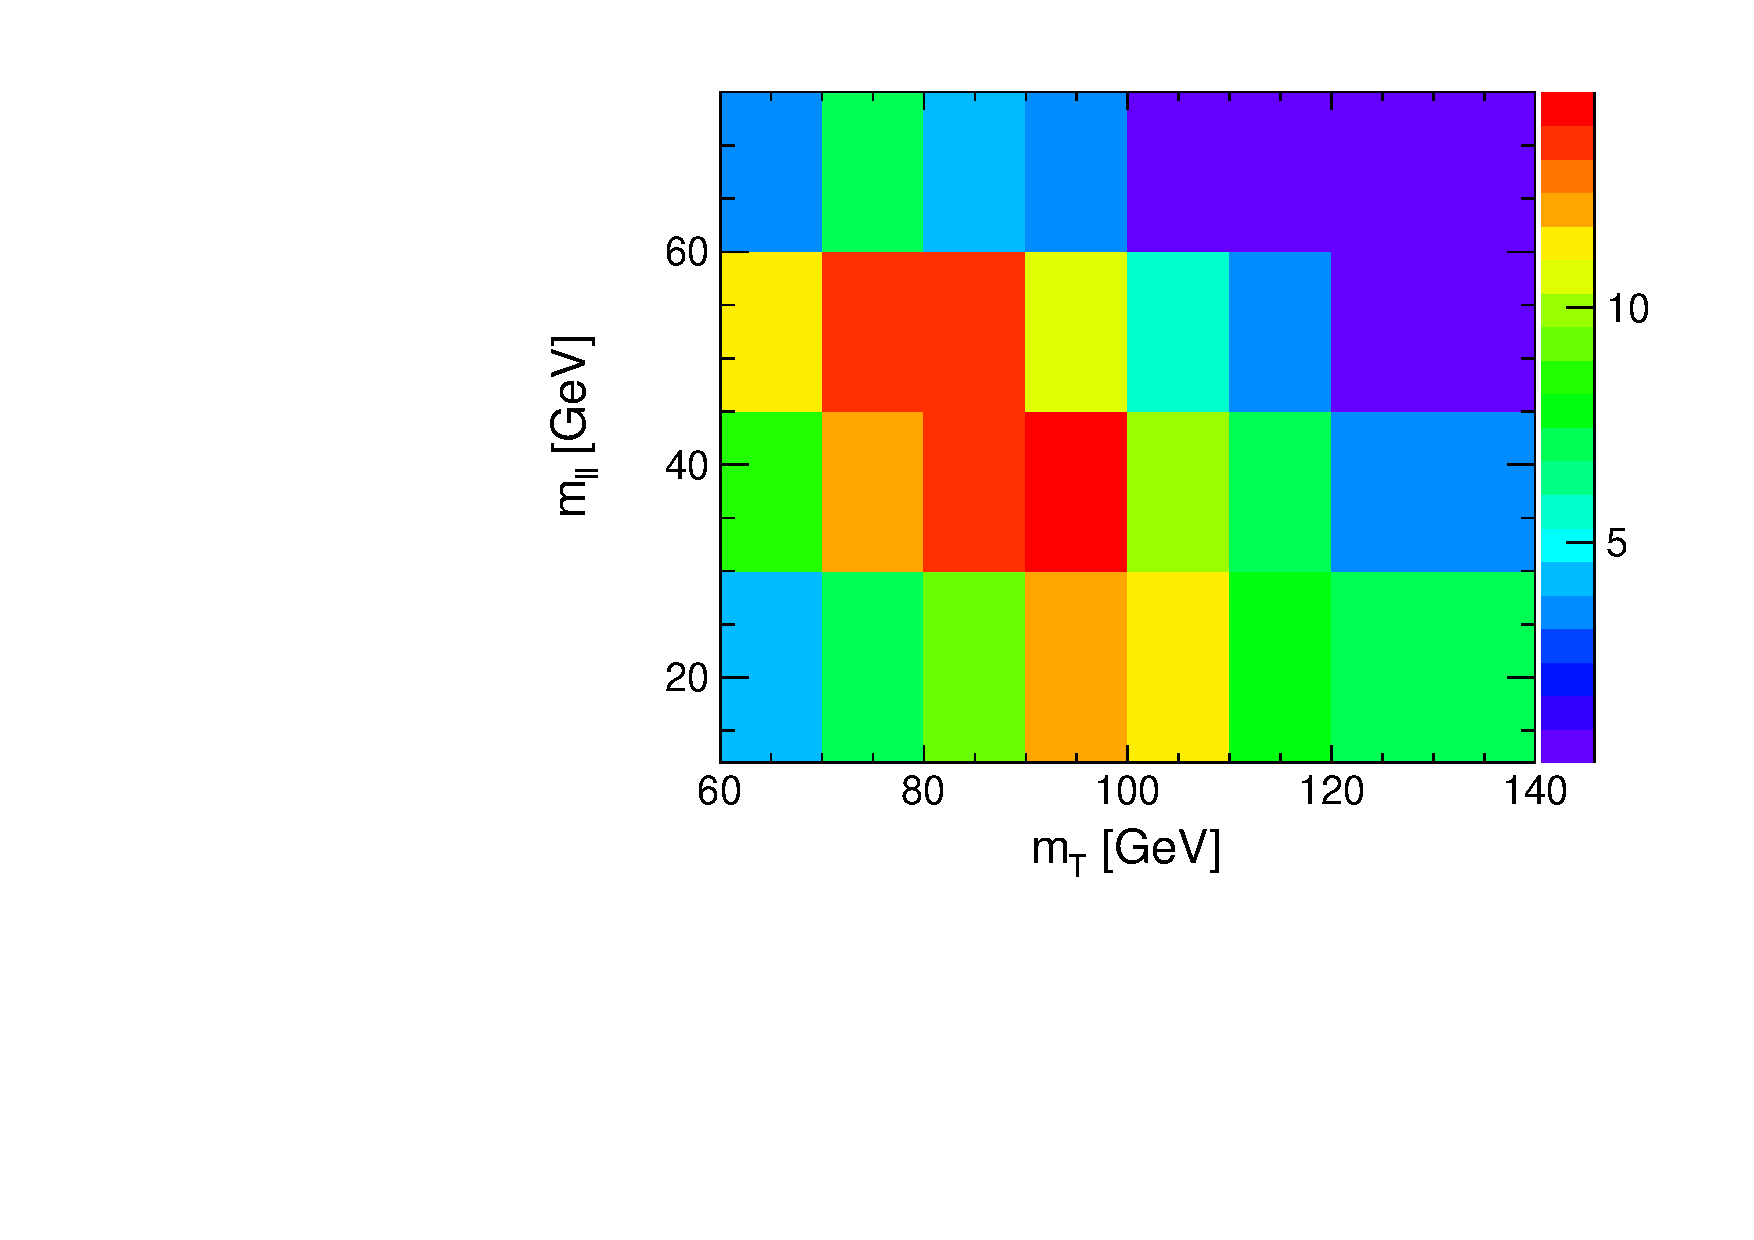
\includegraphics[width=.45\textwidth]{figures/mtvsmll_xww.pdf}
}\\
\caption{The $m_T-m_{\ell\ell}$ templates for the SM Higgs and 
spin 2 graviton like resonances, zoomed in 
the signal regions. The distributions are 
normalized to the expectations for \intlumiEightTeV.}
\label{fig:mtvsmll_sig}
\end{figure}
%%%%%%%%%%%%%%%%%%%%%%%%%%%%%%%%%%%%%%%%%%%%%


%%%%%%%%%%%%%%%%%%%%%%%%%%%%%%%%%%%%%%%%%%%%%
\begin{figure}[!hbtp]
\centering
\subfigure[$qq\to WW$]{
\centering
\label{subfig:qqww}
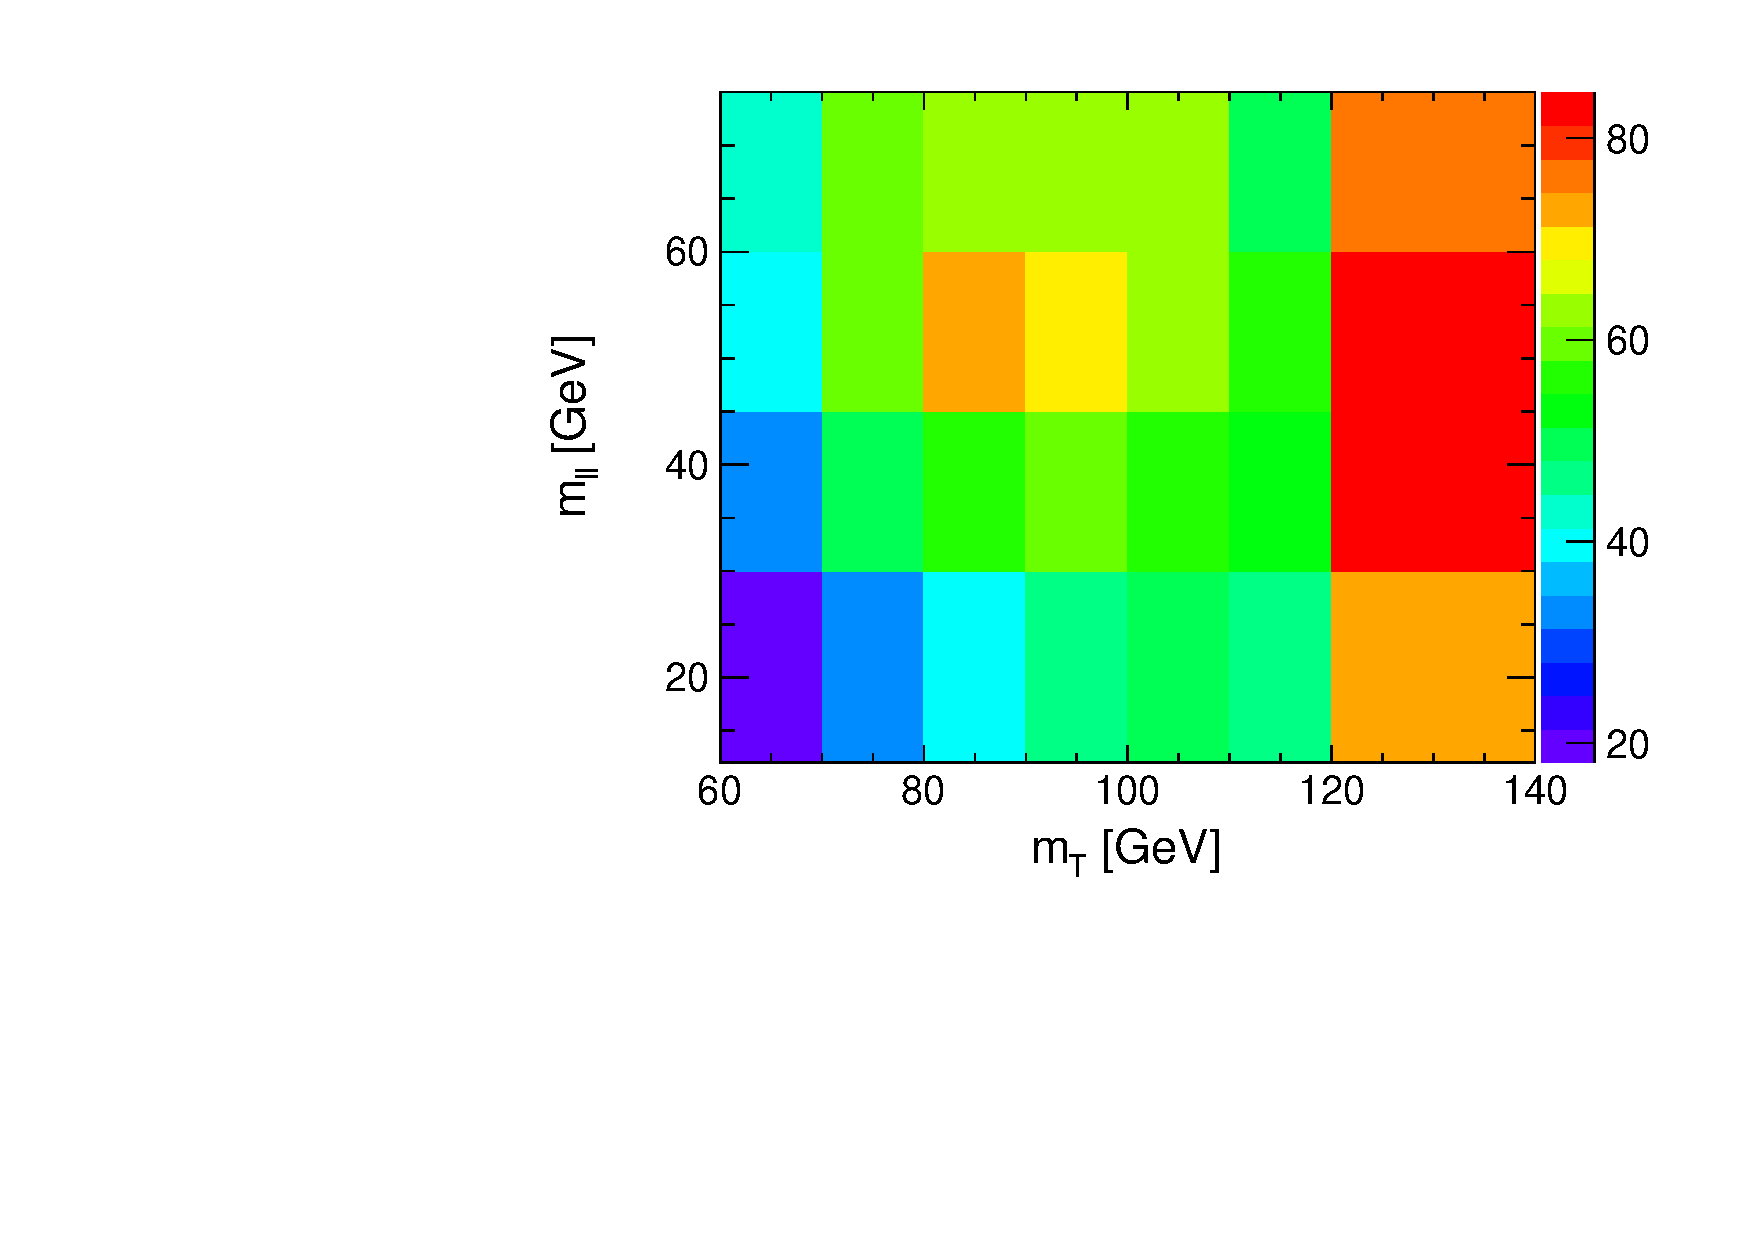
\includegraphics[width=.45\textwidth]{figures/mtvsmll_qqWW.pdf}
}
\subfigure[W+Jets]{
\centering
\label{subfig:wjets}
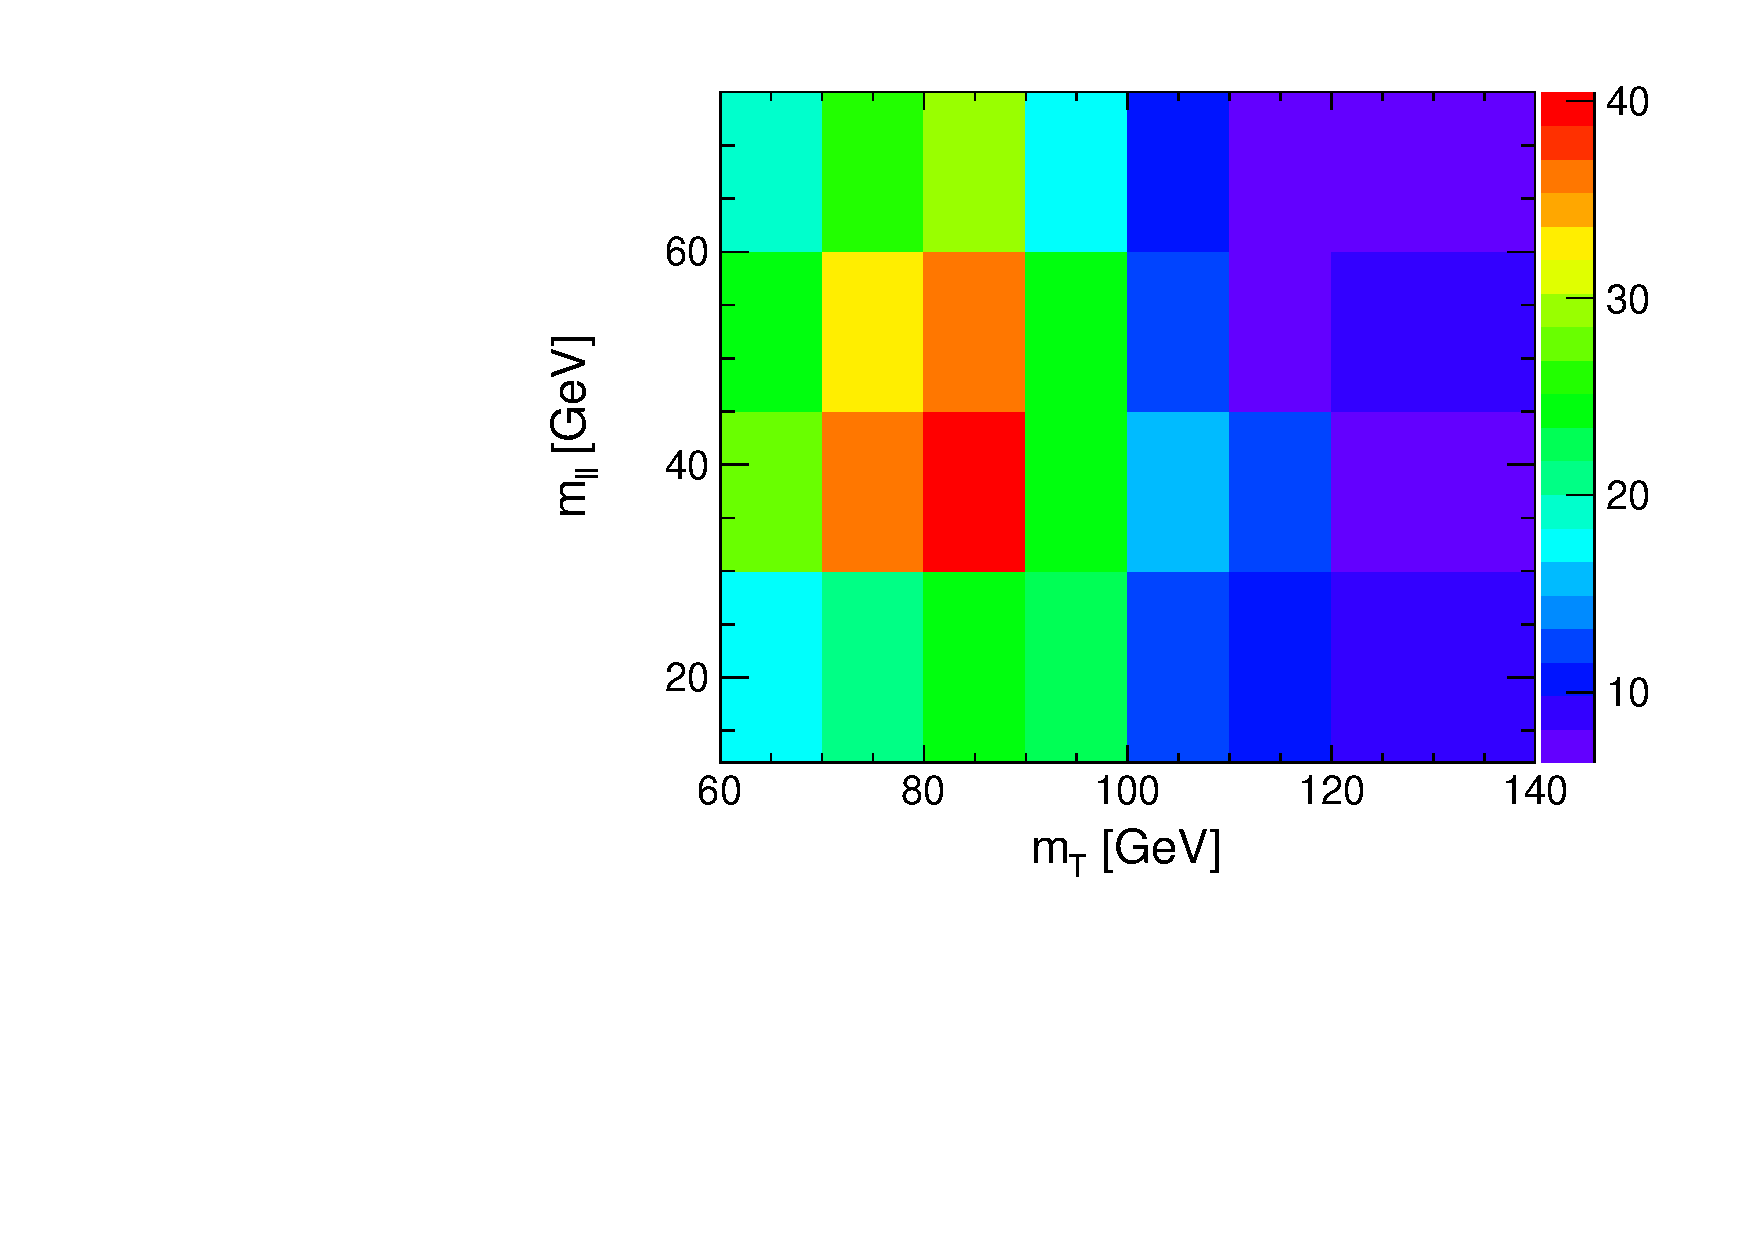
\includegraphics[width=.45\textwidth]{figures/mtvsmll_Wjets.pdf}
}\\
\subfigure[$W\gamma$]{
\centering
\label{subfig:wgamma}
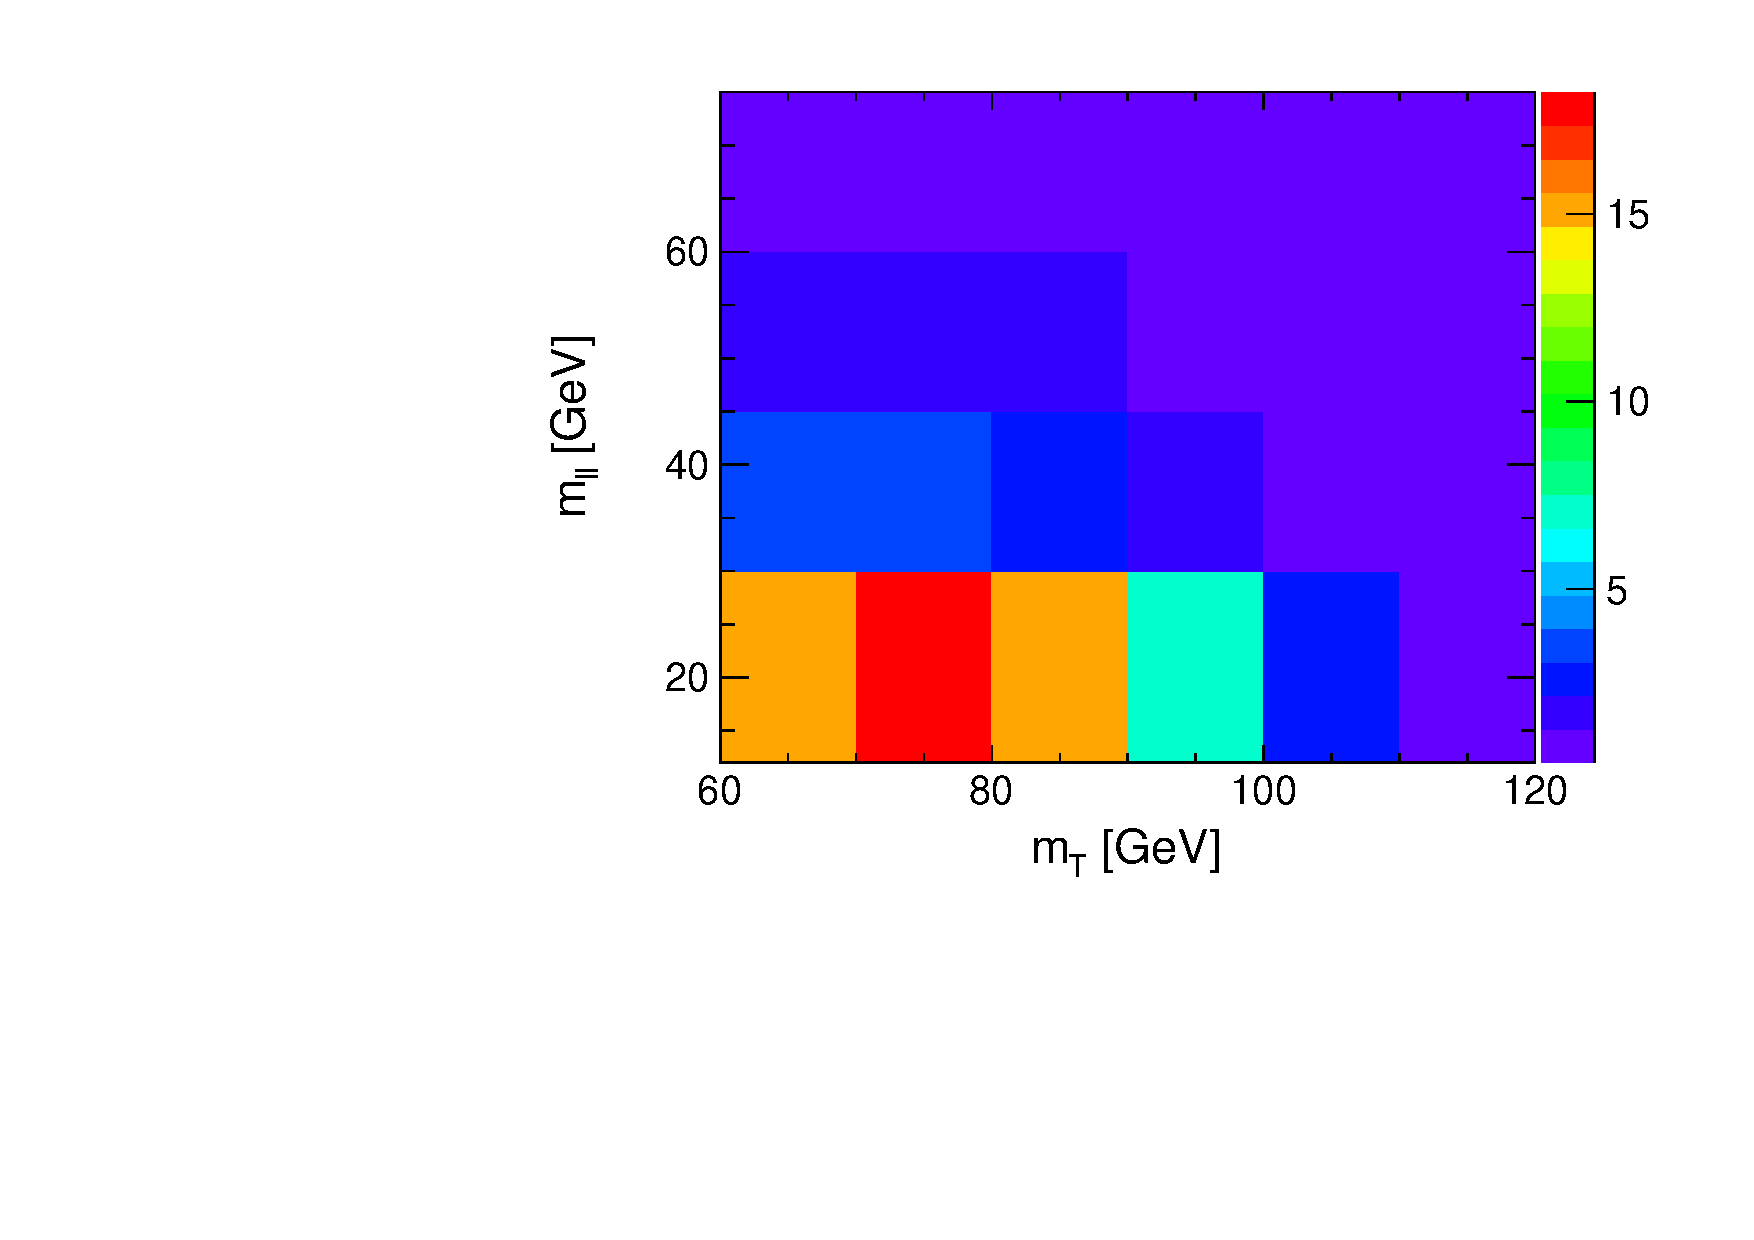
\includegraphics[width=.45\textwidth]{figures/mtvsmll_Wgamma.pdf}
}
\subfigure[$W\gamma^*$]{
\centering
\label{subfig:wgst}
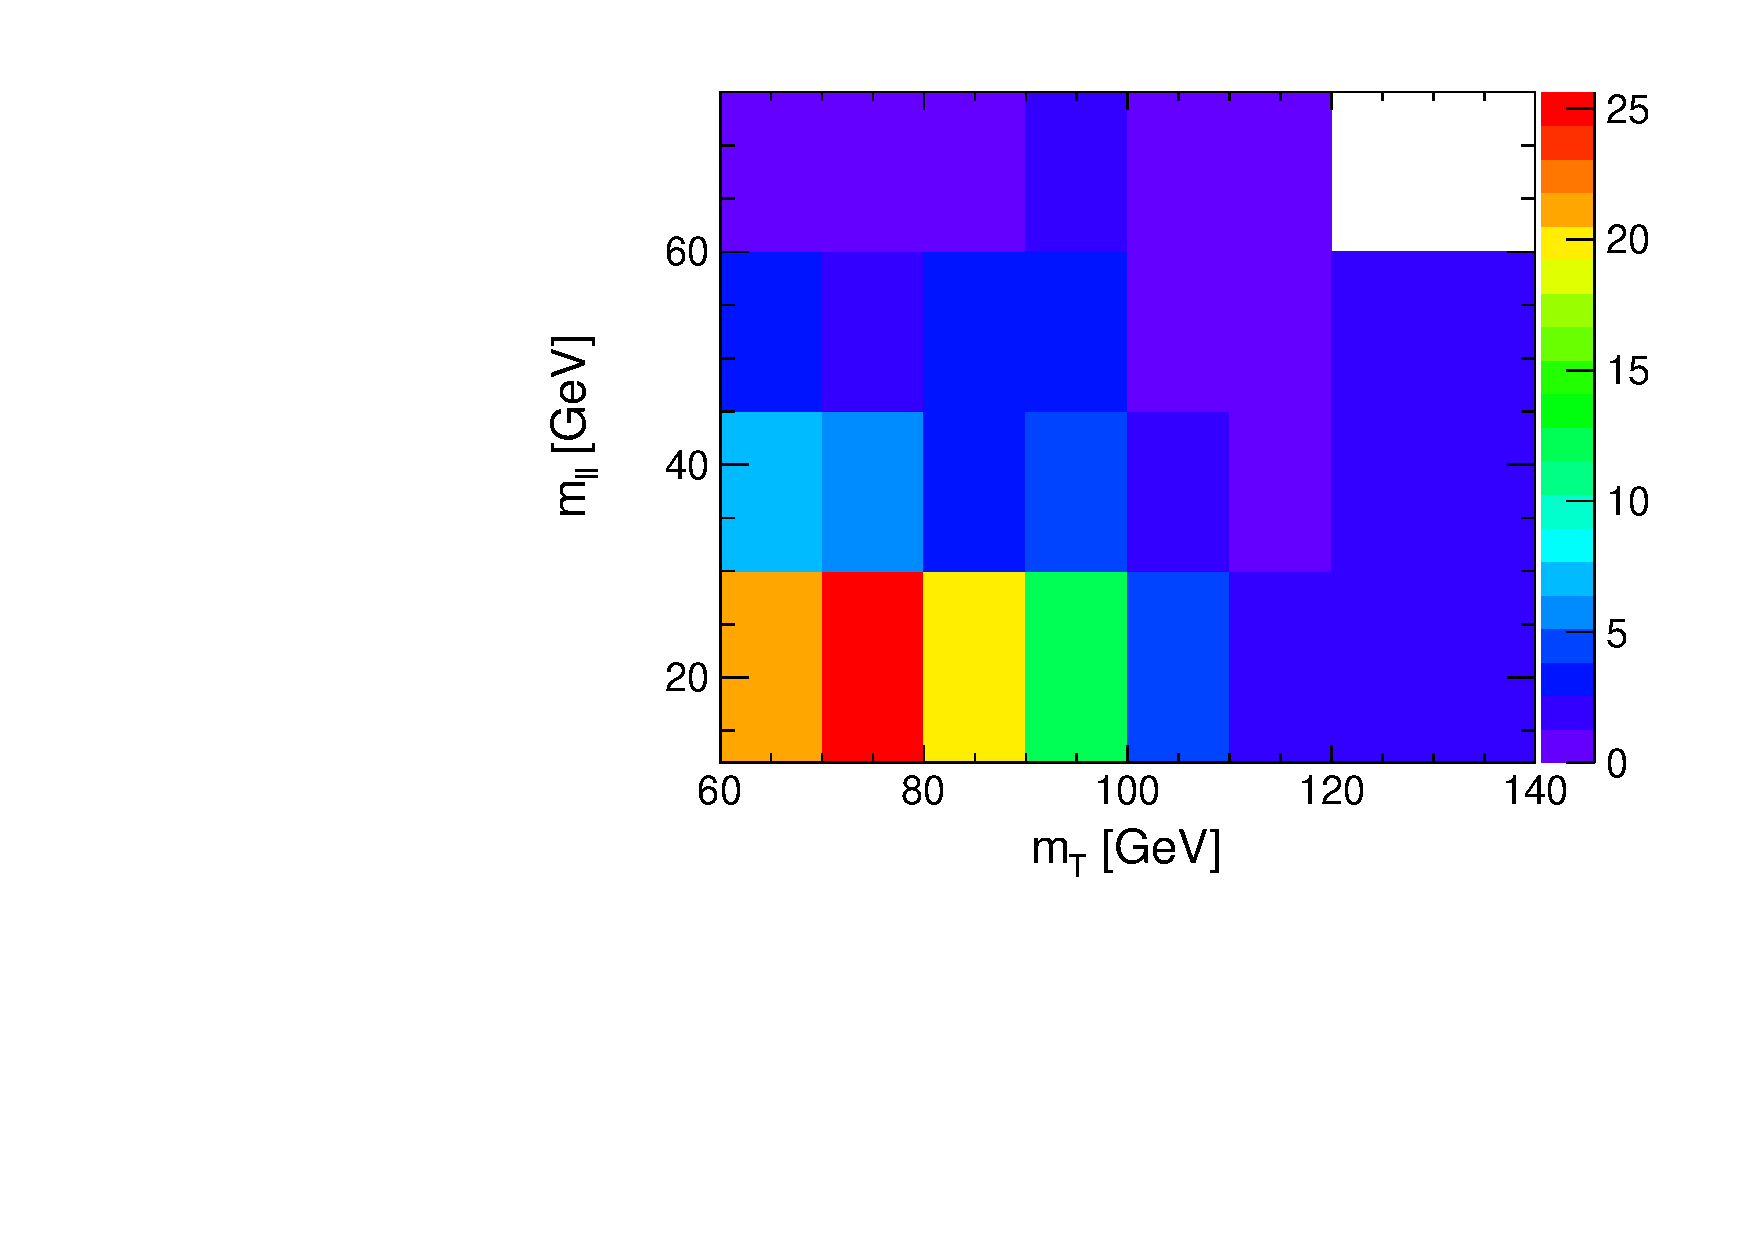
\includegraphics[width=.45\textwidth]{figures/mtvsmll_Wgstar.pdf}
}\\
\subfigure[Top]{
\centering
\label{subfig:top}
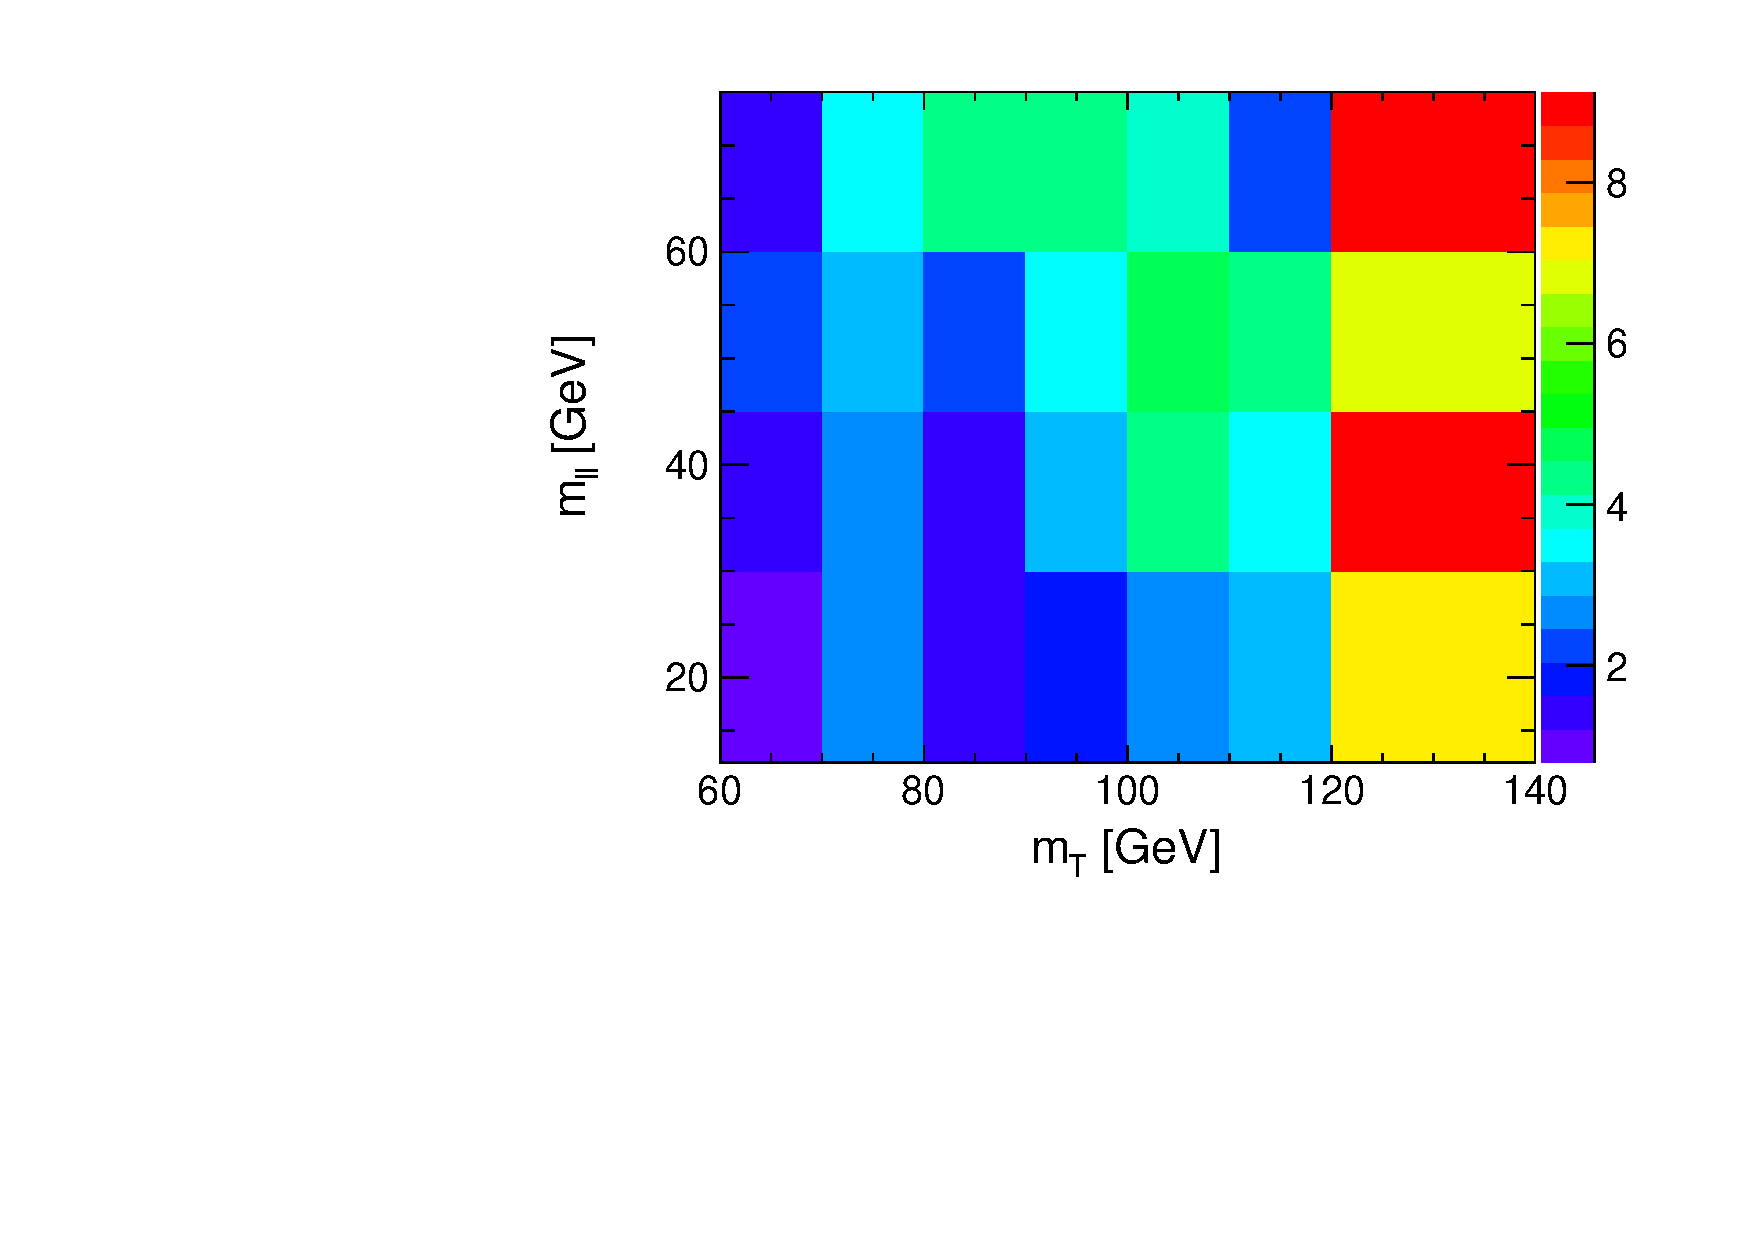
\includegraphics[width=.45\textwidth]{figures/mtvsmll_Top.pdf}
}
\subfigure[VV]{
\centering
\label{subfig:vv}
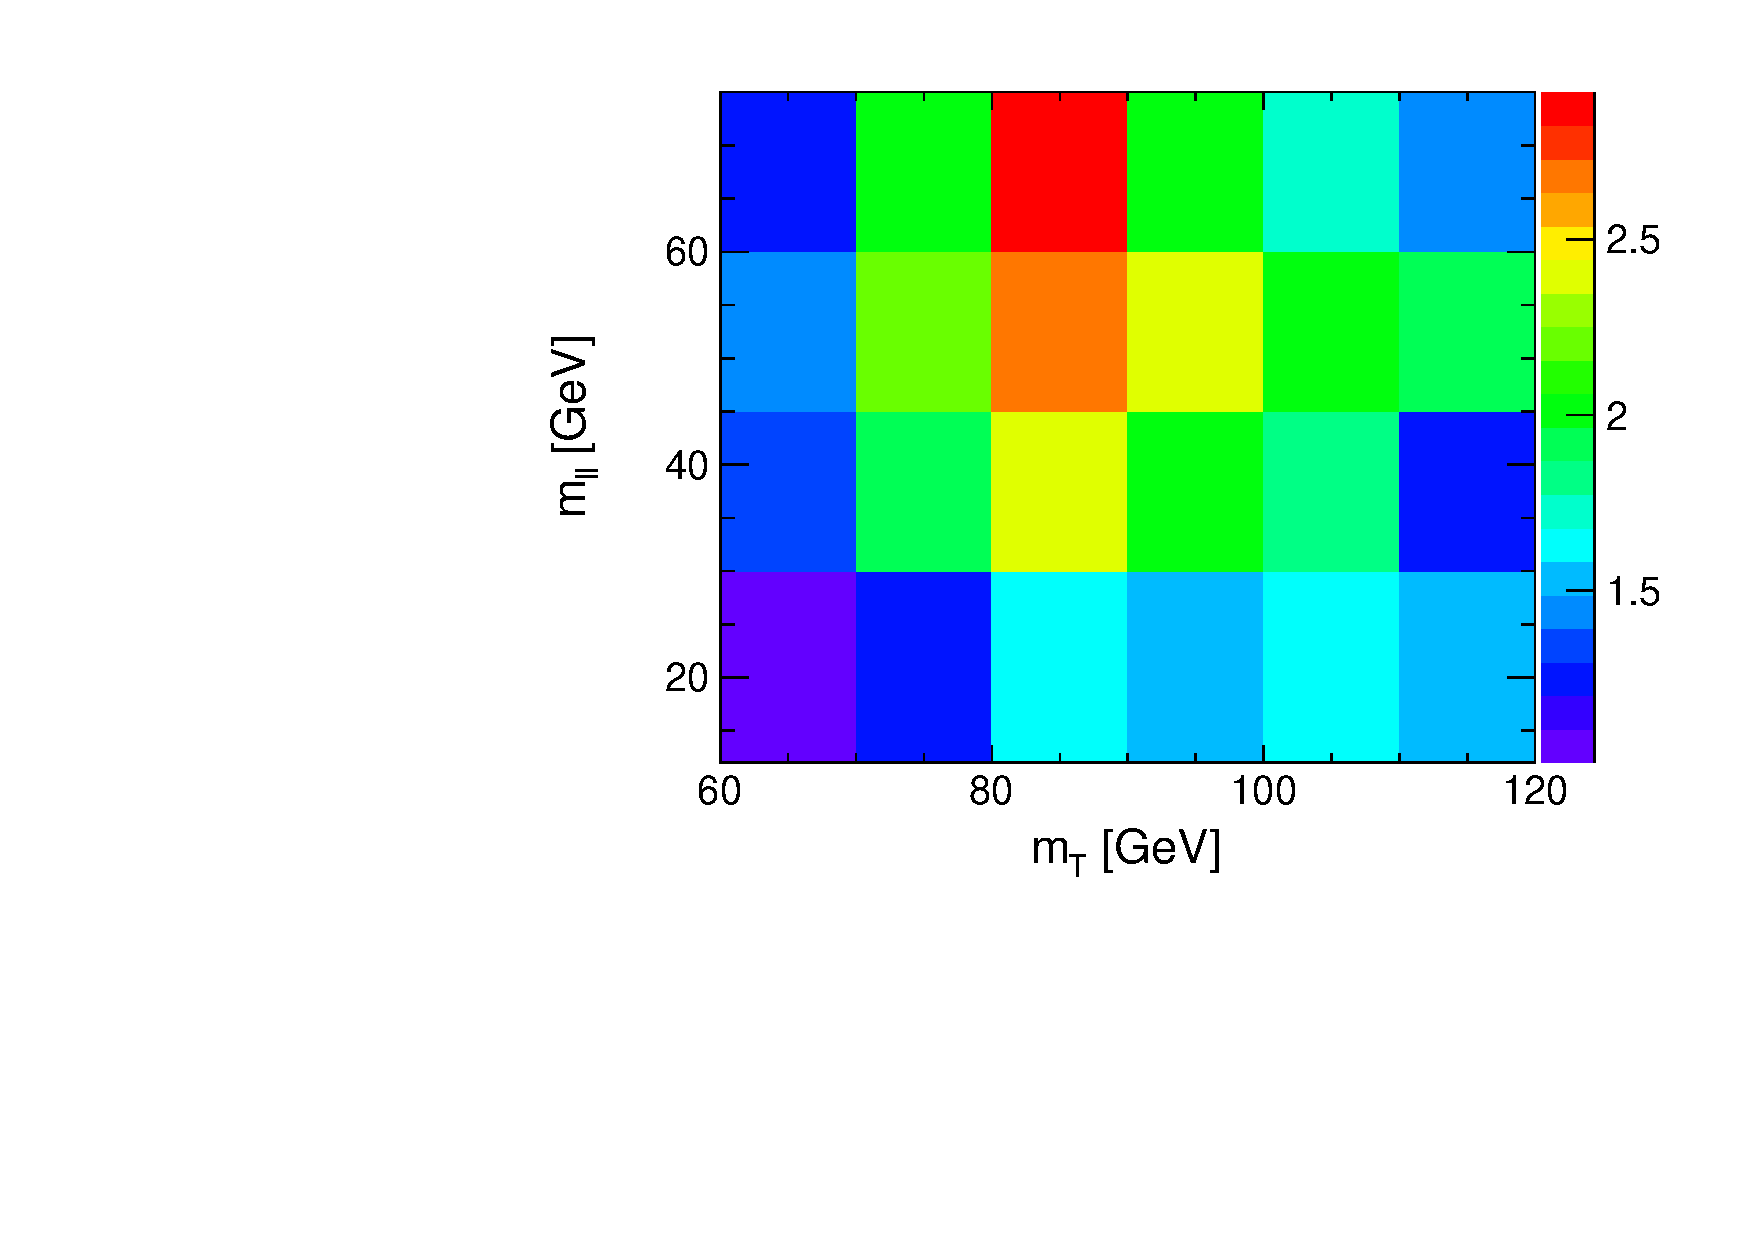
\includegraphics[width=.45\textwidth]{figures/mtvsmll_VV.pdf}
}\\

\caption{The $m_T-m_{\ell\ell}$ templates for the backgrounds, zoomed in 
the signal regions. The distributions are 
normalized to the expectations for \intlumiEightTeV.}
\label{fig:mtvsmll_bkg}
\end{figure}
%%%%%%%%%%%%%%%%%%%%%%%%%%%%%%%%%%%%%%%%%%%%%

\begin{table}[!hbtp]
{%\footnotesize
 %\tiny
 \begin{center}

 \begin{tabular}{| c | c c c c c }
 \hline
 ggH & qqWW & ggWW & VV & Top & Wjets \\ \hline
$210.6\pm43.7$ & $3616.2\pm334.7$ & $190.7\pm58.8$ & $120.8\pm8.7$ & $390.8\pm81.3$ & $831.4\pm299.3$ \\
\hline
\end{tabular}

\vspace{10pt}

 \begin{tabular}{ c c c  | c |}
 \hline
 Wgamma & Wg3l & Ztt & $\sum$Bkg \\ \hline
$100.7\pm30.8$ & $164.7\pm50.4$ & $39.1\pm4.3$ & $5454.4\pm463.9$ \\ 
\hline
\end{tabular}


\end{center}
}
\caption{Expected signal and background yields for \intlumiEightTeV.}
\label{tab:yield}
\end{table}

\clearpage 

\section{Systematic Uncertainties}
\label{sec:systematics}
This analysis does not have any clear mass peak anywhere, hence is to a 
large extent a counting experiment.
Therefore it is important to understand the 
signal efficiency and the background predictions.
We have taken into account the following systematic uncertainties:

\begin{itemize}
\item {\it Luminosity:} We assume an uncertainty of 5.0\%.

\item {\it Lepton identification and trigger efficiencies:} 
We measure the efficiencies in data using the tag and probe method that is described
in detail in Section~\ref{sec:efficiency}. 
The estimated uncertainty is about $2\%$ per lepton leg.

\item {\it Momentum scale:} 
Due to several factors, the energy scale for electrons and the momentum 
scale for muons have relatively large uncertainties in the current data
processing. 
We assign a systematic uncertainty by varying the transverse momentum of the muons by $1\%$, 
and $2\%$ and $5\%$ for electrons in the barrel and the endcap, respectively. 
The contribution to the uncertainty on the dilepton efficiency is about $1.5\%$.

\item {\it $\met$ modeling:} We use a data-driven method to estimate the $\dyll$
background, which is affected by the $\met$ resolution. 
Events with neutrinos giving real $\met$ in the final state also have a small uncertainty. 
We assess this uncertainty on the event selection efficiency by varying the $\met$ in signal events
by an additional $10\%$. We find an uncertainty on the event selection efficiency of around 2\%.

\item {\it Background estimation:} 
The methods to estimate the different backgrounds are explained in 
Section~\ref{sec:backgrounds}.
Here we summarize the systematic uncertainties associated with the methods used.
  \begin{itemize}
  \item $\WW$ Background: the relative uncertainty on this background is about $25-37\%$ for $\intlumiEightTeV$. 
    There is an additional theoretical uncertainty on the $gg \to WW$ contribution, which is around $50\%$.
  \item Jet induced backgrounds, $\Wjets$ and $QCD$: the associated systematic
    uncertainty is 36\%.
  \item Top background: this background is estimated using $b$-tagged events and
    the $b$-tagging efficiency, which is measured in control regions in data.
    The associated systematic uncertainties are below $5\%$, 
    while the statistical component is about $25\%$ for $\intlumiEightTeV$.
  \item Drell-Yan background: The uncertainty arises from the limited knowledge of
    events with large $\met$ tails. 
    We conservatively quantify such uncertainty from the variation of the ratio $R_{out/in}$
    as a function of the $\met$ requirement,
    leading to an estimate of about $50\%$. 
    As very few $\dyll$ events are selected, this has anyhow a small affect on the final analysis results ($\sim1\%$).
  \item Other backgrounds: The sub-dominant backgrounds are estimated from simulation 
    with appropriate systematic uncertainties on their cross section.
    We take $3\%$ for $\WZ$ and $\ZZ$ events. %and $10\%$ for $W+\gamma$ events.
    These uncertainties must be augmented by the luminosity normalization uncertainty.
  \end{itemize}

\item {\it Pileup:} an incorrect modeling of the pileup in the Monte Carlo samples 
can bias the expected event yields. The simulated events have been re-weighted 
on the basis of the number of reconstructed
primary vertices. The re-weighting procedure affects only slightly the results of the analysis,
the event yields changing by $\sim$1\%. The latter is conservatively assumed as 
the corresponding systematic uncertainty. 

\item {\it Higgs cross section:} these uncertainties are taken from the Higgs cross
section working group~\cite{LHCHiggsCrossSectionWorkingGroup:2011ti}. The uncertainty 
on the $gg \to H$ production is about 15\% and it is one of the dominant effects.

\item {\it Jet counting and theoretical uncertainties:} 
we must make sure that the jet multiplicity is well reproduced by our 
simulation because we split our analysis in different jet bins. 
Experimental and theoretical uncertainties are both important.
The experimental jet counting efficiency is measured in data 
using $\dyll$ events. The effect of the statistical uncertainty 
of the jet energy correction measurement on the extrapolation
of the jet counting efficiency from $\dyll$ events to Higgs signal
events is propagated and accounted for as the experimental 
systematic uncertainty. 
We consider the theoretical uncertainties on the Parton Distribution Functions (PDFs), 
the uncertainty due to higher order corrections and the effect of the fragmentation and 
hadronization process. The overall uncertainties on the signal efficiency are 
about $7\%$, $10\%$ and $20\%$ for the 0-jet, 1-jet and 2-jet bins, respectively.
Correlations between different jet bins are taken into account when computing
the upper limits. A detailed discussion of the method and procedures for estimating
theoretical uncertainties on the signal yield can be found in 
Section \ref{sec:theorySystematicsSignal} below.

\item {\it Monte Carlo statistics:} We also take into account the 
size of the simulated event samples. 
This contributes an uncertainty of about $2-3\%$ to the signal
efficiencies, but it is as large as $100\%$ for some background components on specific
Higgs mass points.

\item {\it Shape uncertainties for multivariate analyses:} these uncertainties 
are discussed in detail in~\cite{MVASyst}. We have used those methods 
to estimate them.
\end{itemize}

\subsection{Theoretical Systematic Uncertainties on Signal Efficiency}
\label{sec:theorySystematicsSignal}
The theoretical systematic uncertainties on the signal yield is factorized into the
product of two components, assumed to be independent. The first component is the uncertainty
on the fraction of events categorized into the different jet bins and the effect
of migrations across jet bins. The second component is the uncertainty
on the lepton acceptance and the selection efficiency of all other cuts. The effect of
parton distribution function and the value of $\alpha_{s}$, and the effect of 
higher order corrections are considered for both components. For the jet categorization,
we consider, additionally, the effect of higher order log terms via the uncertainty in the 
parton shower model and the underlying event.

\subsubsection{Systematic Uncertainties on the Jet Bin Fractions}
\label{sec:HiggsJetBinFractionSystematics}
We consider the effect on the jet counting categorization without imposing any additional
selection cuts on the signal. A jet in the event will be counted if it has $p_{T} > 30$ GeV. 
We define the jet bin fractions $f_{0}$, $f_{1}$, $f_{2}$
as the fraction of Higgs events with $0$, $1$, and $2$ or more counted jets. 

The uncertainty due to higher order corrections is evaluated by comparing the effect of
varying the renormalization scale and factorization scale on the jet bin fractions. To 
estimate these jet bin fractions, we combine the inclusive $gg \to H$ production cross section
computed at NNLO \cite{LHCHiggsCrossSectionWorkingGroup:2011ti} ($\sigma_{\geq 0}$) and the 
NLO calculations from MCFM \cite{MCFMHiggsProduction} for the inclusive production cross section 
of $gg \to H+1$jet ($\sigma_{\geq 1}$) and $gg \to H+2$jet ($\sigma_{\geq 2}$), 
through the following relations:

\begin{eqnarray}
\label{eqn:jetBinFractions}
  f_{0} = (\sigma_{\geq 0} - \sigma_{\geq 1} ) / \sigma_{\geq 0} \\
  f_{1} = (\sigma_{\geq 1} - \sigma_{\geq 2} ) / \sigma_{\geq 0} \\
  f_{2} = \sigma_{\geq 2} / \sigma_{\geq 0} \\
\end{eqnarray}

The systematic uncertainties on $\sigma_{\geq 0}$, $\sigma_{\geq 1}$, and $\sigma_{\geq 2}$, are reflected by 
the values of $\kappa_{\geq 0}$, $\kappa_{\geq 1}$, and $\kappa_{\geq 2}$ respectively. 
The central values of the cross sections are computed  using the MSTW2008 NLO parton distribution functions and 
assuming a factorization and renormalization scale of $m_{H} / 2$. The uncertainty on the inclusive
production cross section, $\kappa_{\geq 0}$, is cited from the CERN Yellow Report 
\cite{LHCHiggsCrossSectionWorkingGroup:2011ti}.  The systematic uncertainties
$\kappa_{\geq 1}$, and $\kappa_{\geq 2}$ are estimated by performing the following four variations on
the factorization scale ($\mu_{f}$) and renormalization scale ($\mu_{r}$):

\begin{itemize}
\item: $\mu_{f} = m_{H} $, $\mu_{r} = m_{H}$,
\item: $\mu_{f} = m_{H} / 4$, $\mu_{r} = m_{H} / 4$,
\item: $\mu_{f} = m_{H} $, $\mu_{r} = m_{H} / 2$,
\item: $\mu_{f} = m_{H} / 2$, $\mu_{r} = m_{H} $,

\end{itemize}
using MCFM and evaluating the largest positive and largest negative difference from the central
value for $\sigma_{\geq 1}$ and $\sigma_{\geq 2}$. We symmetrize the uncertainties via the formula:

\begin{eqnarray}
\label{eqn:kappaSymmetrization}
  \kappa_{\mathrm{symmetrized}} = \sqrt{e^{\Delta_{+}} \times e^{\Delta_{-}}} ,
\end{eqnarray}

where $\Delta_{\mathrm{+/-}}$ are the relative positive and negative uncertainty respectively.
The results for $\kappa_{\geq 0}$, $\kappa_{\geq 1}$, and $\kappa_{\geq 2}$ are summarized in Table 
\ref{tab:InclXS_ScaleVariation}.


\begin{table}[!htbp]
\begin{center}
\begin{tabular}{|c|c|c|c|}

\hline
Higgs Mass     &     $\kappa_{\geq 0}$        &   $\kappa_{\geq 1}$        &     $\kappa_{\geq 2}$       \\
\hline
 115 & $ 1.106$  & $ 1.226$  & $ 1.149$  \\
 120 & $ 1.104$  & $ 1.224$  & $ 1.120$  \\
 130 & $ 1.100$  & $ 1.230$  & $ 1.117$  \\
 140 & $ 1.096$  & $ 1.220$  & $ 1.129$  \\
 150 & $ 1.095$  & $ 1.220$  & $ 1.124$  \\
 160 & $ 1.095$  & $ 1.221$  & $ 1.199$  \\
 170 & $ 1.090$  & $ 1.222$  & $ 1.175$  \\
 180 & $ 1.089$  & $ 1.218$  & $ 1.171$  \\
 190 & $ 1.087$  & $ 1.217$  & $ 1.171$  \\
 200 & $ 1.087$  & $ 1.213$  & $ 1.197$  \\
 250 & $ 1.083$  & $ 1.208$  & $ 1.230$  \\
 300 & $ 1.082$  & $ 1.208$  & $ 1.205$  \\
 350 & $ 1.090$  & $ 1.207$  & $ 1.209$  \\
 400 & $ 1.075$  & $ 1.195$  & $ 1.195$  \\
 450 & $ 1.078$  & $ 1.194$  & $ 1.196$  \\
 500 & $ 1.087$  & $ 1.188$  & $ 1.174$  \\
 550 & $ 1.089$  & $ 1.191$  & $ 1.194$  \\
 600 & $ 1.090$  & $ 1.187$  & $ 1.192$  \\

\hline
\end{tabular}
\caption{ $\kappa$ values for the systematic uncertainties due to missing higher order corrections
for the inclusive Higgs production cross section, the inclusive Higgs+1Jet production cross section, 
and inclusive Higgs+2Jet production cross section. }
\label{tab:InclXS_ScaleVariation}
\end{center}
\end{table}

Using the expressions given in Table \ref{tab:JetBinFractionCorrelatedSystematicsFormulas}, we calculate 
the systematic uncertainties expressed in log-normal form on the jet bin fractions $f_{0}$, $f_{1}$, 
and $f_{2}$. There are three systematic uncertainties for each jet bin fraction due to the higher order
corrections on the three inclusive cross section calculations $\sigma_{\geq 0}$, $\sigma_{\geq 1}$, 
and $\sigma_{\geq 2}$, for a total of $9$ systematic uncertainties, of which only $5$ are non-zero.
The values of these $\kappa$'s reflecting the systematic uncertainties and their correlations are 
summarized in Table \ref{tab:JetBinFractionSystematics_ScaleVariation} for all Higgs masses considered.


\begin{table}[!htbp]
\begin{center}
\begin{tabular}{|c|c|c|c|}

\hline
Nuisance Parameter & $\kappa$'s for $0$ jet bin                                                       & $\kappa$'s for $1$ jet bin                                                      & $\kappa$'s for $2$ jet bin                       \\
\hline
QCDscale\_ggH       & $\kappa^{0}_{\mathrm{QCDscale\_ggH}} = (\kappa_{\geq 0})^{\frac{1}{f_{0}}}$                & $1.0$                                                                           & $1.0$                                            \\
\hline
QCDscale\_ggH1in    & $\kappa^{0}_{\mathrm{QCDscale\_ggH1in}} = (\kappa_{\geq 1})^{- \frac{f_{1}+f_{2}}{f_{0}}}$ & $\kappa^{1}_{\mathrm{QCDscale\_ggH1in}} = (\kappa_{\geq 1})^{\frac{f_{1}+f_{2}}{f_{1}}}$  & $1.0$                                            \\
\hline
QCDscale\_ggH2in    & $1.0$                                                                            & $\kappa^{1}_{\mathrm{QCDscale\_ggH2in}} = (\kappa_{\geq 2})^{- \frac{f_{2}}{f_{1}}} $     & $\kappa^{2}_{\mathrm{QCDscale\_ggH2in}} = \kappa_{\geq 2}$ \\
\hline

\end{tabular}
\caption{Table of formulas expressing the $\kappa$ values for the systematic uncertainties on the
jet bin fractions due to the missing higher order corrections on the total inclusive Higgs cross section, 
the inclusive Higgs+1jet cross section, and the inclusive Higgs+2jet cross section, in terms of the 
$\kappa$ values for these cross sections.  }
\label{tab:JetBinFractionCorrelatedSystematicsFormulas}
\end{center}
\end{table}


\begin{table}[!htbp]
\begin{center}
\begin{tabular}{|c|c|c|c|c|c|}

\hline
Higgs Mass     & $\kappa^{0}_{\mathrm{QCDscale\_ggH}}$ & $\kappa^{0}_{\mathrm{QCDscale\_ggH1in}}$ & $\kappa^{1}_{\mathrm{QCDscale\_ggH1in}}$  & $\kappa^{1}_{\mathrm{QCDscale_ggH2in}}$  & $\kappa^{2}_{\mathrm{QCDscale\_ggH2in}}$   \\
\hline
 115 & $ 1.16$  & $ 0.92$  & $ 1.28$  & $ 0.97$  & $ 1.15$  \\
 120 & $ 1.16$  & $ 0.92$  & $ 1.28$  & $ 0.97$  & $ 1.12$  \\
 130 & $ 1.15$  & $ 0.91$  & $ 1.29$  & $ 0.98$  & $ 1.12$  \\
 140 & $ 1.15$  & $ 0.91$  & $ 1.28$  & $ 0.97$  & $ 1.13$  \\
 150 & $ 1.15$  & $ 0.90$  & $ 1.28$  & $ 0.97$  & $ 1.12$  \\
 160 & $ 1.15$  & $ 0.90$  & $ 1.28$  & $ 0.96$  & $ 1.20$  \\
 170 & $ 1.15$  & $ 0.89$  & $ 1.28$  & $ 0.96$  & $ 1.18$  \\
 180 & $ 1.15$  & $ 0.89$  & $ 1.28$  & $ 0.96$  & $ 1.17$  \\
 190 & $ 1.15$  & $ 0.88$  & $ 1.28$  & $ 0.96$  & $ 1.17$  \\
 200 & $ 1.15$  & $ 0.88$  & $ 1.27$  & $ 0.96$  & $ 1.20$  \\
 250 & $ 1.16$  & $ 0.86$  & $ 1.27$  & $ 0.96$  & $ 1.17$  \\
 300 & $ 1.17$  & $ 0.84$  & $ 1.27$  & $ 0.95$  & $ 1.20$  \\
 350 & $ 1.20$  & $ 0.83$  & $ 1.27$  & $ 0.95$  & $ 1.21$  \\
 400 & $ 1.17$  & $ 0.82$  & $ 1.26$  & $ 0.95$  & $ 1.20$  \\
 450 & $ 1.19$  & $ 0.81$  & $ 1.26$  & $ 0.95$  & $ 1.20$  \\
 500 & $ 1.22$  & $ 0.80$  & $ 1.25$  & $ 0.95$  & $ 1.17$  \\
 550 & $ 1.24$  & $ 0.78$  & $ 1.26$  & $ 0.95$  & $ 1.19$  \\
 600 & $ 1.25$  & $ 0.78$  & $ 1.26$  & $ 0.94$  & $ 1.19$  \\

\hline

\end{tabular}
\caption{ Table of $\kappa$ values for the systematic uncertainties for the jet bin 
fractions due to missing higher order corrections for the total inclusive Higgs
cross section, the inclusive Higgs+1jet cross section, and the inclusive Higgs+2jet
cross section. }
\label{tab:JetBinFractionSystematics_ScaleVariation}
\end{center}
\end{table}


%% The uncertainties due to the parton distribution functions and $\alpha_{s}$ on the jet bin fractions 
%% are evaluated using the prescription from the PDF4LHC Recommendations \cite{PDF4LHC}. As for the systematic
%% uncertainties due to missing higher order corrections, we evaluate the effect of the PDF uncertainties 
%% on the value of $\sigma_{\geq 0}$, $\sigma_{\geq 1}$, and $\sigma_{\geq 2}$ and propagate them to 
%% the jet bin fractions using the formulas from Equations \ref{eqn:jetBinFractions}.

Finally, we estimate the systematic uncertainty due to higher order log terms by testing the default 
parton shower and hadronization model, Pythia, with the results obtained using an alternative
parton shower and hadronization model, Herwig. In the first case, Powheg is used for the matrix
element calculation, while in the second case MC@NLO is used. In order to isolate the effect of the 
parton shower and hadronization model, we reweight the Higgs $p_{T}$ distribution to the reference 
NNLO+NNLL resummed calculation, in both cases. Since the underlying event model in the two Monte Carlo 
are also different, this estimate includes also the effect of the underlying event model. 

The relative differences in the jet bin fractions, $f_{0}$, $f_{1}$, and $f_{2}$, 
between the two results are taken as a systematic uncertainty and are 
summarized in Table \ref{tab:JetBinFractionSystematics_PartonShower}.

\begin{table}[!htbp]
\begin{center}
\begin{tabular}{|c|c|c|c|}

\hline
               &   \multicolumn{3}{|c|}{ $\kappa$ values for systematic uncertainties on: } \\
\hline
Higgs Mass     &   $f_{0}$   &  $f_{1}$       &   $f_{2}$       \\
\hline
115 & $0.941$ & $1.128$ & $1.212$ \\
120 & $0.940$ & $1.110$ & $1.293$ \\
130 & $0.937$ & $1.113$ & $1.237$ \\
140 & $0.941$ & $1.104$ & $1.168$ \\
150 & $0.942$ & $1.093$ & $1.156$ \\
160 & $0.943$ & $1.084$ & $1.138$ \\
170 & $0.946$ & $1.075$ & $1.108$ \\
180 & $0.947$ & $1.067$ & $1.092$ \\
190 & $0.948$ & $1.068$ & $1.083$ \\
200 & $0.952$ & $1.055$ & $1.059$ \\
250 & $0.955$ & $1.058$ & $0.990$ \\
300 & $0.958$ & $1.061$ & $0.942$ \\
350 & $0.964$ & $1.068$ & $0.889$ \\
400 & $0.966$ & $1.078$ & $0.856$ \\
450 & $0.954$ & $1.092$ & $0.864$ \\
500 & $0.946$ & $1.102$ & $0.868$ \\
550 & $0.931$ & $1.117$ & $0.861$ \\
600 & $0.920$ & $1.121$ & $0.872$ \\
\hline
\end{tabular}
\caption{Table of $\kappa$ values for the systematic uncertainty on the jet bin fractions
due to  uncertainties in the parton shower and hadronization model and uncertainties
on the model of the underlying event, as a function of the assumed Higgs mass.  }
\label{tab:JetBinFractionSystematics_PartonShower}
\end{center}
\end{table}



\subsubsection{Lepton Acceptance and Selection Efficiency }

The effect of the parton distribution function and the value of $\alpha_{s}$
 on the lepton acceptance and the efficiency of all the selection cuts are 
estimated using the prescription from the PDF4LHC recommendations \cite{PDF4LHC}. We 
propagate the uncertainty for each of the three PDF sets, MSTW2008, CT10, and
NNPDF, according to their own prescriptions, and then take the envelope
of the systematic uncertainties as the total PDF+$\alpha_{s}$  uncertainty. 

%The effect of the missing higher order corrections are accounted for by
%reweighting the Higgs $p_{T}$ spectrum to the one obtained from the
%NNLO+NNLL calculation with the renormalization and factorization scales
%varied by factors of $2$ and $1/2$. 
It is assumed that any change in the
lepton acceptance and the efficiency of other selection cuts are only
influenced via the Higgs $p_{T}$ spectrum. This effect is much smaller in 
magnitude than the effect on the jet bin fractions in any case, and 
essentially can be neglected.



\subsection{Summary of Systematic Uncertainties}
All systematic uncertainties taken into account in this analysis
are summarized in Table~\ref{tab:systhww}, although they should be taken as 
guidelines, the actual values depend on this Higgs mass hypothesis. 
The total uncertainty depends on the Higgs mass and jet bin considered,
however is typically $15\%$ on the background estimation and about $20\%$ 
on the signal efficiency. The uncertainties are treated as log-normal 
distributions, and hence the values are of the order of one unit. It is worth 
noting there are several systematic uncertainties which include an effect 
not only on the normalization, but also on the shape of the multivariate output 
classifier, as discussed in~\cite{MVASyst}.

\begin{table}[ht!]
\begin{center}
\caption{\label{tab:systhww} Summary of all systematic uncertainties (relative). As most of the 
systematic uncertainties are evaluated separately for each higgs mass at each jet bins, 
the values quoted here reflect a rough range of given quantities. More details on 
the systematic errors evaluated for the background normalization can be found in 
Section~\ref{sec:dataresults}. }
\vspace{5pt}
{\footnotesize
\begin{tabular}{l|c|c|c|c|c|c|c|c}
\hline
%&       \multicolumn{8}{|c|}{Relative Uncertainty (\%)} \\
%Source      &                            $H \to \WW$ & $qq \to \WW$ & $gg \to \WW$ & $VV$ non-$\Z$ resonant & top & $\dyll$ & $\Wjets$ & $V(W/Z)+\gamma$    \\              
\multirow{2}{*}{Source} & $H $ & $qq \to$ & $gg \to$  & non-$\Z$ resonant & top & DY & $\Wjets$ & $V(W/Z)+\gamma$    \\
                        & $\to WW$   & $\WW$    & $\WW$       & $VV$              &     &         &       &                     \\
\hline

\hline
Luminosity                    & 5.0 & --- & --- & 5.0 & --- & --- & ---  &  5.0  \\
Trigger efficiencies          & 1.5 & 1.5 & 1.5 & 1.5 & --- & --- & ---  &  1.5  \\
Muon efficiency               & 1.5 & 1.5 & 1.5 & 1.5 & --- & --- & ---  &  1.5  \\
Electron id efficiency        & 2.5 & 2.5 & 2.5 & 2.5 & --- & --- & ---  &  2.5  \\
Momentum scale                & 1.5 & 1.5 & 1.5 & 1.5 & --- & --- & ---  &  1.5  \\
$\met$ resolution             & 2.0 & 2.0 & 2.0 & 2.0 & 2.0 & 3.0 & ---  &  1.0  \\
PDF uncertainties             & 7.2 & 4.0 & 4.0 & 4.0 & --  & --  & ---  &  --  \\ 
QCD scale uncertainties       &15-25 & -- & -- & 4.0 & -- & --  & --- & --  \\ 
%Jet counting                 &15-25& --- & 5.4 & 5.4 & --- & --- & ---  &  5.4  \\  
%Higgs cross section          & 5-15& --- & --- & --- & --- & --- & --- \\ %&  ---  \\
%$WZ/ZZ$ cross section         & --- & --- & --- & 3.0 & --- & --- & --- &  ---  \\
$qq \to WW$ norm.             & --- &  15 & --- & --- & --- & --- & --- &  ---  \\
$gg \to WW$ norm.             & --- & --- &  30 & --- & --- & --- & ---  &  ---  \\
$\Wjets$ norm.                & --- & --- & --- & --- & --- & --- &  36  &  ---  \\
$W\gamma/\gamma^*$ norm.      & --- & --- & --- & --- & --- & --- &  --- & 30   \\
top  norm.                    & --- & --- & --- & --- & 10-25 & --- & ---  &  ---  \\
$\dyll$ norm.                 & --- & --- & --- & --- & --- & 20-100 & ---  &  ---  \\
%Monte Carlo statistics        & 2-5 &	4  &  6  &   4 &   6 &  20 &  -   \\ %&  10   \\
\hline
\end{tabular}
}
\end{center}
\end{table}


\section{Expected Sensitivity}
\label{sec:expresults}
In this section we document the expected separatoins between 
the SM Higgs and spin 2 graviton hypothesis ($2_\text{min}^+$) calculated for \intlumiEightTeV 
at 8 TeV.  

Figure~\ref{fig:expsep} shows the distributions of 
$q=-2\text{ln}({\cal L}_{2_\text{min}^+}/{\cal L}_{\text{0}^+})$
with generated samples of background and signal of two types, 
SM $0^+$ and minimal couplings spin 2 $2_\text{min}^+$, for $m_H=$125 GeV. 
Here the likelihoods, $\cal L$, are calculated with the signal rates 
allowed to float indepdently for each signal type and the nusiance 
parameters are treated as independent. 
The expected distributions are generated with the same number of events 
after the full event selections. 
The mean of the expected SM $0^+$ distribution is x.x standard deviations 
in the tail of the $2_\text{min}^+$ distribution, while 
the mean of the expected $2_\text{min}^+$ distribution is x.x standard deviations 
in the tail of the $0^+$ distribution. 
The signal to background significance expected on average 
for the SM Higgs hypothesis is $3.3\sigma$, while for the spin 2 graviton $2_\text{min}^+$ 
model it is around $2.6\sigma$. 

%%%%%%%%%%%%%%%%%%%%%%%%%%%%%%%%%%%%%%%%%%%%%
\begin{figure}[!hbtp]
\centering
\label{subfig:res}
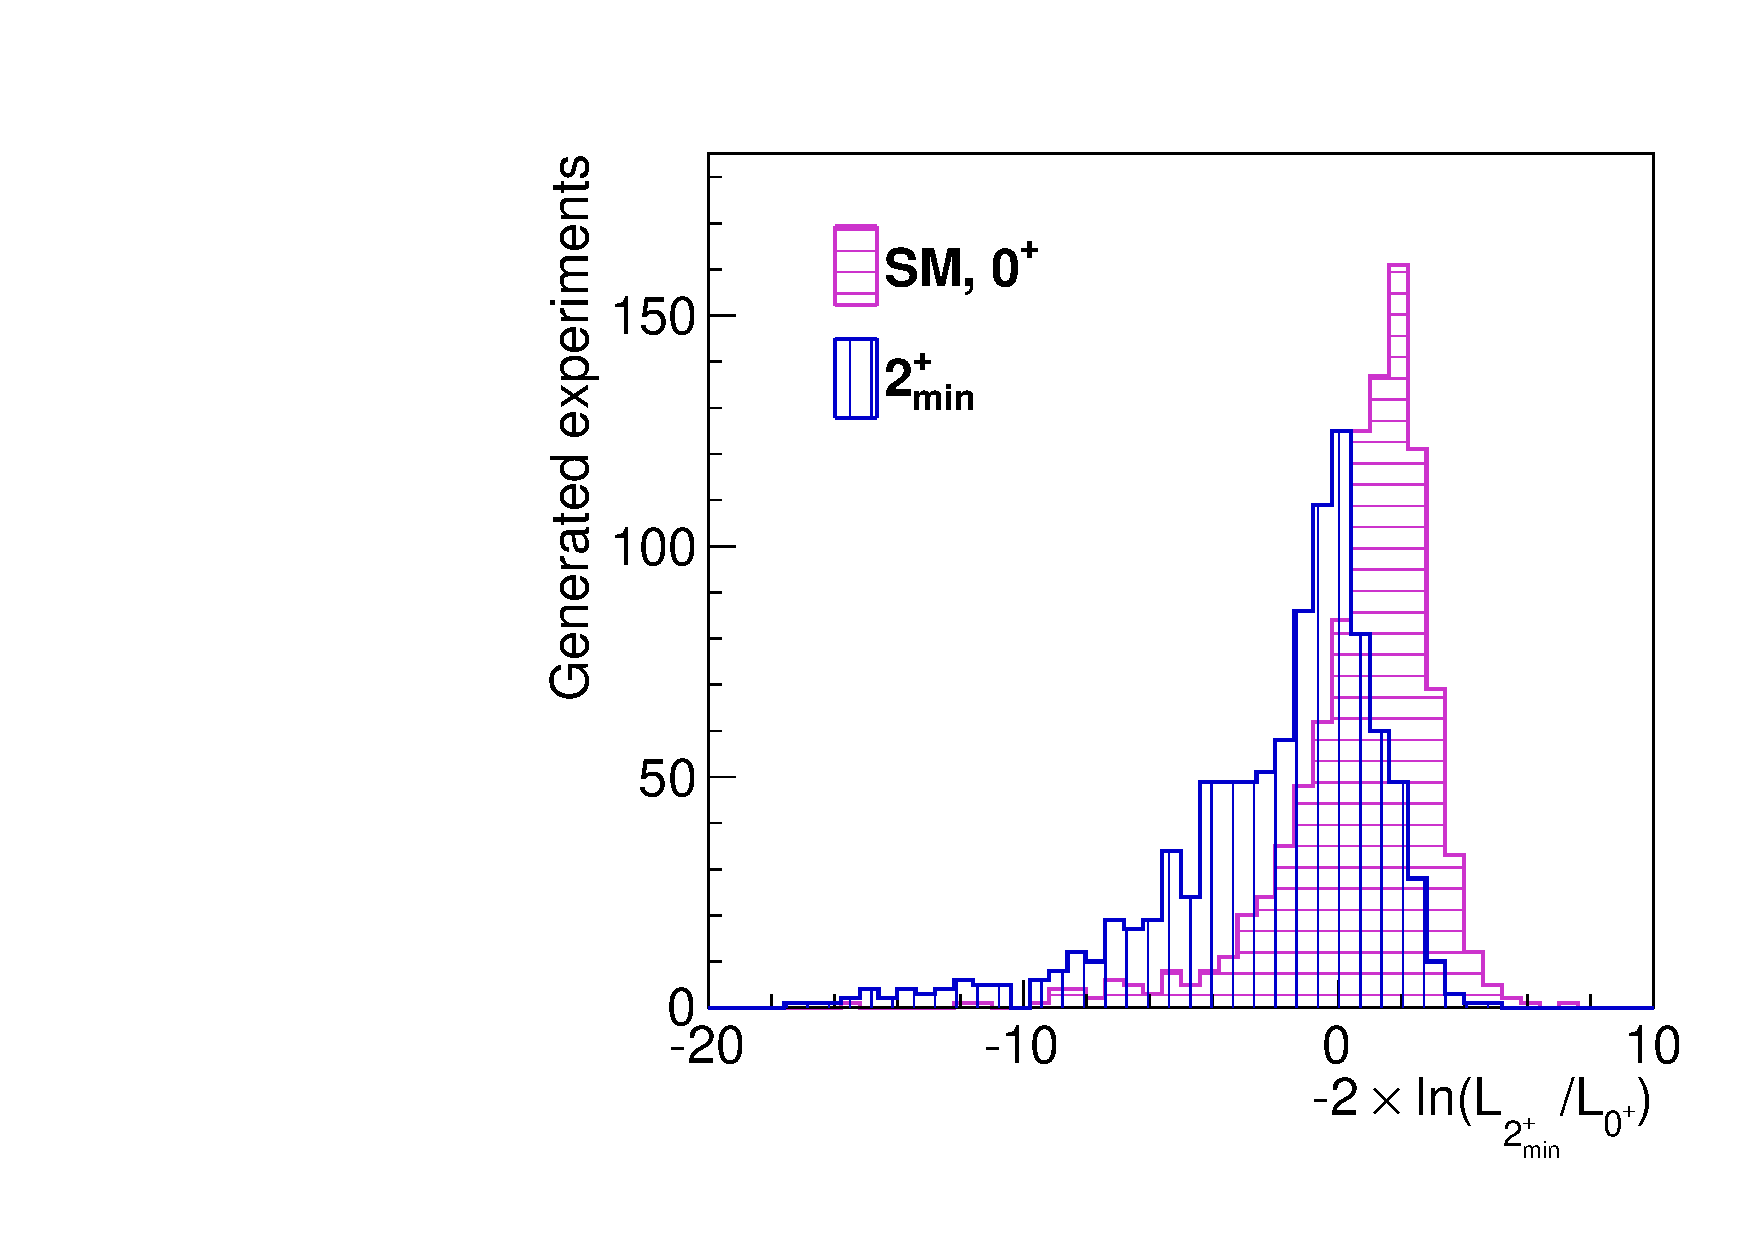
\includegraphics[width=.45\textwidth]{figures/hypo_separation_12fb.pdf}
\caption{Distributions of 
$q=-2\text{ln}({\cal L}_{2_\text{min}^+}/{\cal L}_{\text{0}^+})$, 
for two signal types ($0^+$ horizontally hatched histogram, 
$2_\text{min}^+$ vertically hatched histogram) for $m_H=$125 GeV. 
In these distributions 10,000 pseudo-datasets are generated for 
both hypotheses. }
\label{fig:expsep}
\end{figure}
%%%%%%%%%%%%%%%%%%%%%%%%%%%%%%%%%%%%%%%%%%%%%

%\section{Results}
%\label{sec:dataresults}

\section{Summary}
\label{sec:summary}

We have performed a measurement of the $W^+W^-$ production cross-section
using an integrated luminosity of $\intlumi$ of $pp$ collision data at $\sqrt{s} = $
7~$\TeV$. The measurement was performed in the \wwlnln{} final state.
The $W^+W^-$ production cross-section was measured to be:

\begin{equation*}
\sigma_{WW}  = 53.95 \pm 2.05~\mathrm{(stat.)} \pm 4.30~\mathrm{(syst.)} \pm 2.43~\mathrm{(lumi.)~pb},
\end{equation*}

to be compared with the standard model prediction \cite{Campbell:2011bn}:

\begin{equation*}
\sigma_{WW}  = 47 \pm 2 ~\mathrm{pb}.
\end{equation*}




%===================================================================================================
\clearpage

\vspace*{-0.2cm}
\thebibliography{12}

\bibitem{pdg}
 K. Nakamura et al. (Particle Data Group), "Review of particle physics", J. Phys.G37 , 2010.

\bibitem{Higgs1}
F. Englert and R. Brout, "Broken symmetries and the masses of gauge bosons", Phys. Rev. Lett. 13,  1964.

\bibitem{Higgs2}
P. W. Higgs, "Broken symmetry and the mass of gauge vector mesons", Phys. Rev. Lett. 13, 1964.

\bibitem{Higgs3}
Guralnik, G.S. and Hagen, C.R. and Kibble, T.W.B., "Global Conservation Laws and Massless Particles", 
Phys.Rev.Lett. 13, 1964.

\bibitem{dittmar}
M.~Dittmar and H.~K.~Dreiner, Phys.\ Rev.\  D {\bf 55} (1997) 167".

\bibitem{HWW2010}
CMS Collaboration, "Measurement of WW Production and Search for the Higgs Boson in 
pp Collisions at $\sqrt{s}$ = 7 TeV", arXiv:1102.5429

\bibitem{HWW2011AN}
L.~Bauerdick et al, "A Higgs Boson Search in the Fully Leptonic $W^+W^-$ Final State", CMS AN-2011/155

\bibitem{VBTFCrossSectionNote}
J. Alcaraz Maestre, \textit{et al.}, "Updated Measurements of Inclusive W and Z Cross Sections 
at $\sqrt{s}=7$ TeV", CMS AN-2010/264.

\bibitem{ggWWError}
F.~ Stoeckli, "http://indico.cern.ch/getFile.py/access?contribId=0\&resId=1\&materialId=slides\&confId=49009", 
EWK Diboson meeting of March 12 2009.

\bibitem{json}
{\small
/afs/cern.ch/cms/CAF/CMSCOMM/COMM\_DQM/certification/Collisions11/7TeV/Prompt/Cert\_160404-163869\_7TeV\_PromptReco\_Collisions11\_JSON.txt
}

\bibitem{ElIso}
A. Vartak, M. LeBourgeois, V. Sharma, "Lepton Isolation in the CMS Tracker, ECAL and HCAL", CMS AN-2010/106.

\bibitem{PVDA}
W. Erdmann, M. LeBourgeois, B. Mangano, 
https://indico.cern.ch/getFile.py/access?contribId=5\&sessionId=3\&resId=1\&materialId=slides\&confId=127127, 
note in preparation.

\bibitem{NExpHits}
B. Mangano \textit{et al.}, "Improvement in Photon Conversion Rejection Performance Using 
Advanced Tracking Tools", AN-10-283.

\bibitem{fakeLeptonNote1}
S.~Xie, \textit{et al.}", "Study of Data-Driven Methods for Estimation of Fake Lepton Backgrounds", 
CMS AN-2009/120.

\bibitem{fakeLeptonNote2}
W.~Andrews, \textit{et al.}, "Fake Rates for dilepton Analyses", CMS AN-2010/257.

\bibitem{fakeLeptonBkgSpillage1}
 F. Golf, D. Evans, J. Mulmenstadt  \textit{et al.}, ``Expectations for observation of top quark pair production in the dilepton final state with the early CMS data'', CMS AN-2009/050.

\bibitem{dyestnote}
W. Andrews, et al., “A Method to Measure the Contribution of $\dyll$ to a di-lepton+ MET Selection”, CMS AN-2009/023 (2009).

\bibitem{jes}
CMS Collaboration, "Jet Energy Calibration with Photon+Jet Events", PAS JME-09-004.

\bibitem{jetpas}
CMS Collaboration, "Jet Performance in pp Collisions at $\sqrt{s}=7 \rm\ TeV$", PAS JME-10-003.

\bibitem{btag}
CMS collaboration, "Commissioning of b-jet identification with pp collisions at $\sqrt{s}=7~\TeV$, BTV-10-001.

\bibitem{antikt}
Cacciari, Matteo and Salam, Gavin P. and Soyez, Gregory, "The anti-$k_t$ jet clustering 
algorithm", JHEP 04,  2008.

\bibitem{ConversionNote}
W.~Andrews, \textit{et al.}, "Study of photon conversion rejection at CMS", CMS AN-2009/159.

\bibitem{tmva}
A. Hoecker, \textit{et al.}, "TMVA - Toolkit for Multivariate Data Analysis", arXiv:physics/0703039, 2007.

\bibitem{XS}
CMS Generator group, Standard Model Cross Sections for CMS at 7 TeV, 2010.

\bibitem{PDF4LHC}
PDF4LHC Working Group, 
{\tt http://www.hep.ucl.ac.uk/pdf4lhc/PDF4LHCrecom.pdf}

\bibitem{Nadolsky:2008zw}
Nadolsky, Pavel M. and others, "Implications of CTEQ global analysis for 
collider observables", Phys. Rev. D78 2008.

\bibitem{Martin:2009iq}
Martin, A. D. and Stirling, W. J. and Thorne, R. S. and Watt, G., "Parton 
distributions for the LHC, Eur. Phys. J. C63 2009.

\bibitem{Ball:2010de}
Ball, Richard D. and others, "A first unbiased global NLO determination 
of parton distributions and their uncertainties", arXiv 1002.4407.

\bibitem{bayesian}
A. O'Hagan and J.J. Forster, "Bayesian Inference", Kendall's Advanced Theory of Statistics, 
Arnold, London, 2B, 2004.

\bibitem{ref:tagprobe_mit_w}
G. Bauer {\it et. al.}, "Lepton ef?iencies for the inclusive W cross section measurement with 36.1pb$^{-1}$", AN2011/097

\bibitem{ref:tagprobe_snt_top}
W. Andrews {\it et. al.}, "Uncertainties on the Lepton Selection Efficiency for t$t\bar{t}$ Cross Section Analysis", AN2010/274

\bibitem{LHCHiggsCrossSectionWorkingGroup:2011ti}
LHC Higgs Cross Section Working Group, "Handbook of LHC Higgs Cross Sections: 
Inclusive Observables", CERN-2011-002, 2011.

\bibitem{PFMET} 
CMS Collaboration, ``CMS MET Performance in Events Containing Electroweak Bosons from pp Collisions at $\sqrt{s}=7$ TeV'', CMS PAS JME-2010-005 (2010)


\bibitem{trkMET} 
Marco Zanetti, ``MET with PU in $\hww\to2\ell$'', https://indico.cern.ch/conferenceDisplay.py?confId=131580
Benjamin Hooberman, ``MET with PU in MC and First 2011 Data'', https://indico.cern.ch/contributionDisplay.py?contribId=5\&confId=132579. 


\bibitem{lands}
Mingshui Chen and Andrey Korytov, https://mschen.web.cern.ch/mschen/lands/

\bibitem{MCFMHiggsProduction}
J. Campbell, R.K. Ellis, G. Zanderighi, ``Next-to-Leading order Higgs + 2 jet production via gluon fusion.'', JHEP 0610:028 (2006), hep-ph/0608194

\bibitem{MCFMVVProduction}
J. Campbell, R.K. Ellis, C. Williams, ``Vector boson pair production at the LHC.'', arxiv:hep-ph/1105.0020.

\bibitem{MITHggNote} 
G. Bauer et al., ``Higgs Search in the pp $\rightarrow$ H $\rightarrow$ $\gamma\gamma$ channel at $\sqrt{s}=7$ TeV'', CMS AN-2011/168. 


%===================================================================================================

\clearpage 

\end{document}
